%! TEX encoding = utf8
\chapter{Odpowiedzi skokowe}

Rozważamy 5 różnych wartości skoku: \num{1.0}, \num{2.0}, \num{3.0}, \num{4.0}, \num{5.0}.

\section{Opowiedzi skokowe toru U-Y}

\begin{figure}[H]
\centering
% This file was created by matlab2tikz.
%
%The latest updates can be retrieved from
%  http://www.mathworks.com/matlabcentral/fileexchange/22022-matlab2tikz-matlab2tikz
%where you can also make suggestions and rate matlab2tikz.
%
\definecolor{mycolor1}{rgb}{0.00000,0.44700,0.74100}%
\definecolor{mycolor2}{rgb}{0.85000,0.32500,0.09800}%
\definecolor{mycolor3}{rgb}{0.92900,0.69400,0.12500}%
\definecolor{mycolor4}{rgb}{0.49400,0.18400,0.55600}%
\definecolor{mycolor5}{rgb}{0.46600,0.67400,0.18800}%
%
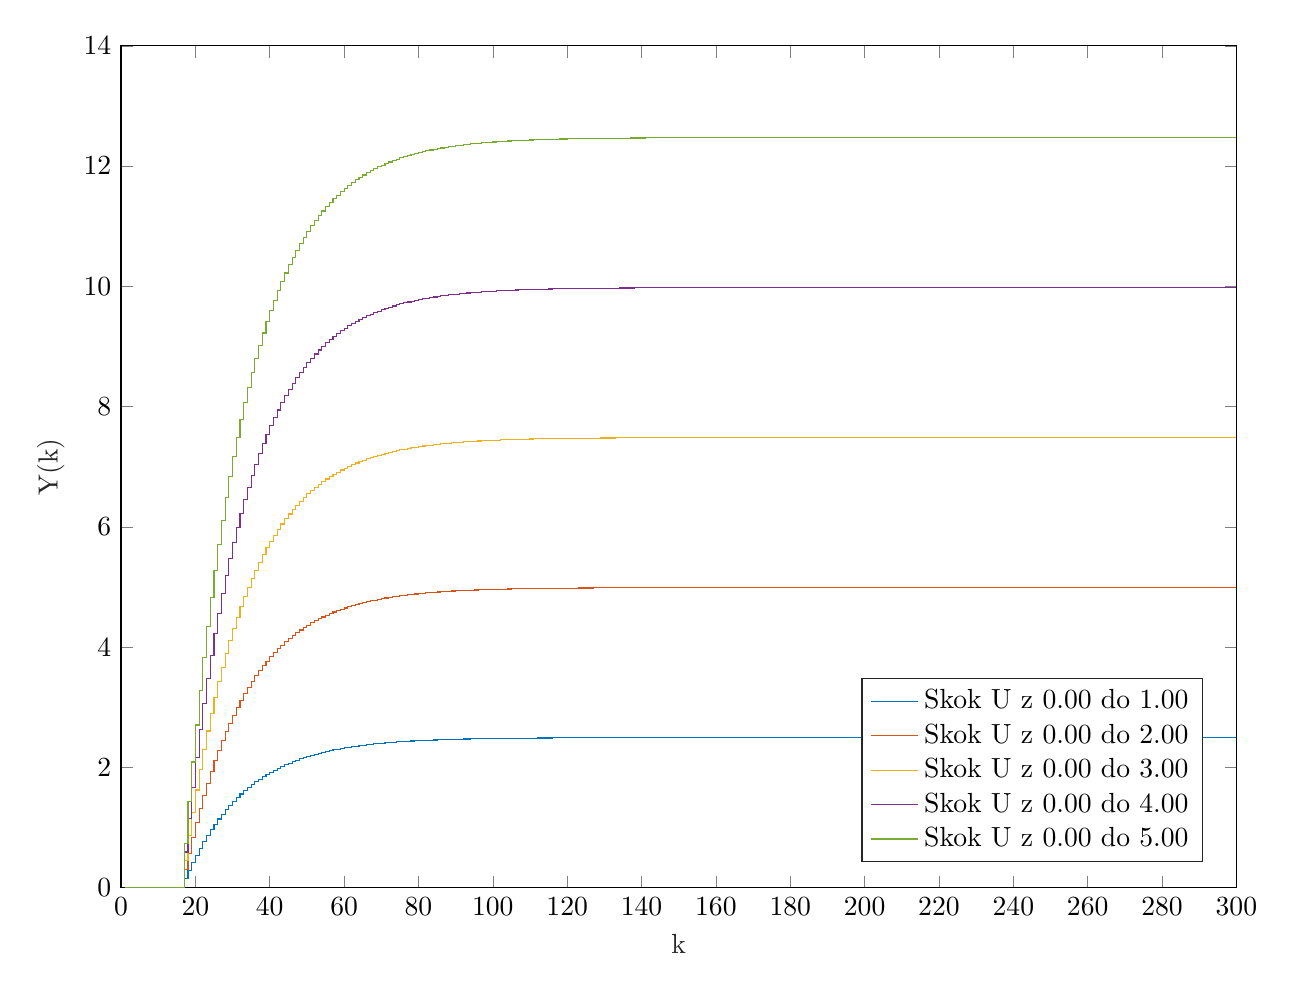
\begin{tikzpicture}

\begin{axis}[%
width=5.577in,
height=4.209in,
at={(0.768in,0.433in)},
scale only axis,
xmin=0,
xmax=300,
xlabel style={font=\color{white!15!black}},
xlabel={k},
ymin=0,
ymax=14,
ylabel style={font=\color{white!15!black}},
ylabel={Y(k)},
axis background/.style={fill=white},
legend style={at={(0.97,0.03)}, anchor=south east, legend cell align=left, align=left, draw=white!15!black}
]
\addplot[const plot, color=mycolor1] table[row sep=crcr] {%
1	0\\
2	0\\
3	0\\
4	0\\
5	0\\
6	0\\
7	0\\
8	0\\
9	0\\
10	0\\
11	0\\
12	0\\
13	0\\
14	0\\
15	0\\
16	0\\
17	0.14788\\
18	0.287003368\\
19	0.4178875887248\\
20	0.541019681620169\\
21	0.656857981328252\\
22	0.765833815583596\\
23	0.868353086271741\\
24	0.964797759090307\\
25	1.05552726696406\\
26	1.14087983209031\\
27	1.2211737112286\\
28	1.29670836859919\\
29	1.36776558051679\\
30	1.43461047566053\\
31	1.4974925146662\\
32	1.55664641252315\\
33	1.61229300706489\\
34	1.6646400766589\\
35	1.71388311002751\\
36	1.76020603096696\\
37	1.8037818805757\\
38	1.84477345945558\\
39	1.88333393220961\\
40	1.91960739642823\\
41	1.95372941823058\\
42	1.98582753630976\\
43	2.01602173631893\\
44	2.04442489733007\\
45	2.07114321199739\\
46	2.09627658196347\\
47	2.11991898995759\\
48	2.14215884995146\\
49	2.16307933665916\\
50	2.18275869559299\\
51	2.20127053481677\\
52	2.2186840994719\\
53	2.23506453008862\\
54	2.25047310563613\\
55	2.26496747220972\\
56	2.27860185820011\\
57	2.29142727674155\\
58	2.30349171618796\\
59	2.31484031932293\\
60	2.32551555196791\\
61	2.33555736161404\\
62	2.34500332666624\\
63	2.35388879685375\\
64	2.3622470253288\\
65	2.37010929294415\\
66	2.37750502517179\\
67	2.38446190209753\\
68	2.39100596190081\\
69	2.39716169820485\\
70	2.40295215165975\\
71	2.40839899609941\\
72	2.41352261959357\\
73	2.41834220069678\\
74	2.42287578017859\\
75	2.42714032850259\\
76	2.43115180930567\\
77	2.43492523911456\\
78	2.43847474352232\\
79	2.44181361003448\\
80	2.44495433778203\\
81	2.44790868428693\\
82	2.45068770945463\\
83	2.45330181695808\\
84	2.45576079316756\\
85	2.45807384377197\\
86	2.46024962822822\\
87	2.46229629216758\\
88	2.46422149788002\\
89	2.46603245299044\\
90	2.46773593743402\\
91	2.46933832883159\\
92	2.47084562635968\\
93	2.47226347320473\\
94	2.47359717768524\\
95	2.47485173312098\\
96	2.47603183652342\\
97	2.47714190617744\\
98	2.47818609817987\\
99	2.47916832199701\\
100	2.48009225509899\\
101	2.48096135672601\\
102	2.48177888083776\\
103	2.48254788829452\\
104	2.48327125831562\\
105	2.48395169925794\\
106	2.48459175875496\\
107	2.48519383325411\\
108	2.4857601769884\\
109	2.48629291041548\\
110	2.48679402815619\\
111	2.48726540646188\\
112	2.48770881023874\\
113	2.48812589965527\\
114	2.48851823635772\\
115	2.48888728931666\\
116	2.48923444032666\\
117	2.48956098917959\\
118	2.48986815853095\\
119	2.49015709847745\\
120	2.49042889086289\\
121	2.49068455332858\\
122	2.49092504312342\\
123	2.49115126068779\\
124	2.49136405302485\\
125	2.49156421687177\\
126	2.49175250168271\\
127	2.49192961243486\\
128	2.4920962122679\\
129	2.49225292496687\\
130	2.49240033729765\\
131	2.4925390012039\\
132	2.49266943587359\\
133	2.4927921296829\\
134	2.49290754202472\\
135	2.49301610502877\\
136	2.49311822517946\\
137	2.49321428483788\\
138	2.4933046436734\\
139	2.49338964001034\\
140	2.4934695920947\\
141	2.49354479928574\\
142	2.4936155431768\\
143	2.49368208864968\\
144	2.49374468486638\\
145	2.49380356620202\\
146	2.49385895312237\\
147	2.49391105300933\\
148	2.4939600609374\\
149	2.49400616040409\\
150	2.49404952401695\\
151	2.49409031413988\\
152	2.49412868350103\\
153	2.49416477576464\\
154	2.49419872606899\\
155	2.49423066153234\\
156	2.49426070172891\\
157	2.4942889591366\\
158	2.49431553955811\\
159	2.49434054251712\\
160	2.49436406163089\\
161	2.49438618496083\\
162	2.49440699534216\\
163	2.49442657069415\\
164	2.49444498431178\\
165	2.49446230514023\\
166	2.49447859803301\\
167	2.49449392399478\\
168	2.49450834040979\\
169	2.4945219012567\\
170	2.49453465731073\\
171	2.49454665633373\\
172	2.49455794325308\\
173	2.49456856032983\\
174	2.49457854731699\\
175	2.49458794160836\\
176	2.49459677837853\\
177	2.4946050907146\\
178	2.49461290974005\\
179	2.49462026473128\\
180	2.49462718322725\\
181	2.49463369113254\\
182	2.4946398128144\\
183	2.49464557119396\\
184	2.49465098783205\\
185	2.49465608300993\\
186	2.49466087580524\\
187	2.49466538416342\\
188	2.4946696249649\\
189	2.49467361408832\\
190	2.49467736646996\\
191	2.49468089615971\\
192	2.49468421637361\\
193	2.49468733954338\\
194	2.49469027736297\\
195	2.49469304083232\\
196	2.49469564029856\\
197	2.49469808549475\\
198	2.49470038557633\\
199	2.49470254915539\\
200	2.49470458433291\\
201	2.49470649872912\\
202	2.49470829951201\\
203	2.49470999342416\\
204	2.49471158680801\\
205	2.4947130856296\\
206	2.4947144955009\\
207	2.49471582170082\\
208	2.49471706919499\\
209	2.49471824265435\\
210	2.49471934647263\\
211	2.4947203847828\\
212	2.49472136147257\\
213	2.49472228019891\\
214	2.49472314440176\\
215	2.49472395731691\\
216	2.49472472198814\\
217	2.49472544127856\\
218	2.49472611788139\\
219	2.49472675432998\\
220	2.49472735300737\\
221	2.49472791615517\\
222	2.49472844588193\\
223	2.4947289441711\\
224	2.49472941288838\\
225	2.49472985378879\\
226	2.49473026852315\\
227	2.49473065864435\\
228	2.4947310256131\\
229	2.49473137080342\\
230	2.49473169550779\\
231	2.49473200094199\\
232	2.49473228824964\\
233	2.4947325585065\\
234	2.49473281272447\\
235	2.49473305185541\\
236	2.49473327679469\\
237	2.49473348838454\\
238	2.4947336874172\\
239	2.49473387463791\\
240	2.49473405074766\\
241	2.49473421640586\\
242	2.49473437223277\\
243	2.49473451881185\\
244	2.49473465669193\\
245	2.49473478638926\\
246	2.49473490838947\\
247	2.49473502314935\\
248	2.4947351310986\\
249	2.49473523264141\\
250	2.49473532815797\\
251	2.49473541800593\\
252	2.49473550252169\\
253	2.49473558202172\\
254	2.49473565680367\\
255	2.49473572714755\\
256	2.49473579331675\\
257	2.49473585555901\\
258	2.49473591410739\\
259	2.49473596918112\\
260	2.49473602098639\\
261	2.49473606971718\\
262	2.49473611555596\\
263	2.49473615867435\\
264	2.4947361992338\\
265	2.49473623738617\\
266	2.49473627327433\\
267	2.49473630703263\\
268	2.49473633878749\\
269	2.4947363686578\\
270	2.4947363967554\\
271	2.49473642318549\\
272	2.49473644804705\\
273	2.49473647143315\\
274	2.49473649343136\\
275	2.49473651412405\\
276	2.49473653358869\\
277	2.49473655189816\\
278	2.49473656912103\\
279	2.49473658532178\\
280	2.49473660056106\\
281	2.49473661489594\\
282	2.49473662838009\\
283	2.49473664106399\\
284	2.49473665299515\\
285	2.49473666421824\\
286	2.49473667477526\\
287	2.49473668470577\\
288	2.49473669404693\\
289	2.49473670283372\\
290	2.49473671109904\\
291	2.49473671887384\\
292	2.49473672618723\\
293	2.4947367330666\\
294	2.49473673953769\\
295	2.49473674562475\\
296	2.49473675135056\\
297	2.49473675673656\\
298	2.49473676180292\\
299	2.49473676656861\\
300	2.49473677105147\\
};
\addlegendentry{Skok U z 0.00 do 1.00}

\addplot[const plot, color=mycolor2] table[row sep=crcr] {%
1	0\\
2	0\\
3	0\\
4	0\\
5	0\\
6	0\\
7	0\\
8	0\\
9	0\\
10	0\\
11	0\\
12	0\\
13	0\\
14	0\\
15	0\\
16	0\\
17	0.29576\\
18	0.574006736\\
19	0.8357751774496\\
20	1.08203936324034\\
21	1.3137159626565\\
22	1.53166763116719\\
23	1.73670617254348\\
24	1.92959551818061\\
25	2.11105453392813\\
26	2.28175966418062\\
27	2.44234742245721\\
28	2.59341673719839\\
29	2.73553116103359\\
30	2.86922095132107\\
31	2.9949850293324\\
32	3.1132928250463\\
33	3.22458601412978\\
34	3.32928015331779\\
35	3.42776622005501\\
36	3.52041206193391\\
37	3.6075637611514\\
38	3.68954691891116\\
39	3.76666786441923\\
40	3.83921479285646\\
41	3.90745883646116\\
42	3.97165507261952\\
43	4.03204347263787\\
44	4.08884979466015\\
45	4.14228642399477\\
46	4.19255316392695\\
47	4.23983797991519\\
48	4.28431769990292\\
49	4.32615867331833\\
50	4.36551739118597\\
51	4.40254106963354\\
52	4.43736819894381\\
53	4.47012906017723\\
54	4.50094621127227\\
55	4.52993494441944\\
56	4.55720371640022\\
57	4.58285455348311\\
58	4.60698343237593\\
59	4.62968063864585\\
60	4.65103110393581\\
61	4.67111472322808\\
62	4.69000665333247\\
63	4.70777759370751\\
64	4.7244940506576\\
65	4.74021858588829\\
66	4.75501005034357\\
67	4.76892380419506\\
68	4.78201192380161\\
69	4.79432339640971\\
70	4.80590430331949\\
71	4.81679799219881\\
72	4.82704523918714\\
73	4.83668440139355\\
74	4.84575156035719\\
75	4.85428065700519\\
76	4.86230361861134\\
77	4.86985047822912\\
78	4.87694948704464\\
79	4.88362722006896\\
80	4.88990867556407\\
81	4.89581736857385\\
82	4.90137541890926\\
83	4.90660363391616\\
84	4.91152158633513\\
85	4.91614768754394\\
86	4.92049925645644\\
87	4.92459258433517\\
88	4.92844299576005\\
89	4.93206490598087\\
90	4.93547187486805\\
91	4.93867665766318\\
92	4.94169125271936\\
93	4.94452694640945\\
94	4.94719435537047\\
95	4.94970346624195\\
96	4.95206367304685\\
97	4.95428381235487\\
98	4.95637219635974\\
99	4.95833664399401\\
100	4.96018451019798\\
101	4.96192271345203\\
102	4.96355776167551\\
103	4.96509577658904\\
104	4.96654251663124\\
105	4.96790339851589\\
106	4.96918351750991\\
107	4.97038766650823\\
108	4.97152035397679\\
109	4.97258582083097\\
110	4.97358805631239\\
111	4.97453081292376\\
112	4.97541762047747\\
113	4.97625179931054\\
114	4.97703647271543\\
115	4.97777457863332\\
116	4.97846888065332\\
117	4.97912197835918\\
118	4.97973631706191\\
119	4.9803141969549\\
120	4.98085778172577\\
121	4.98136910665717\\
122	4.98185008624684\\
123	4.98230252137558\\
124	4.98272810604971\\
125	4.98312843374354\\
126	4.98350500336543\\
127	4.98385922486972\\
128	4.9841924245358\\
129	4.98450584993373\\
130	4.98480067459529\\
131	4.9850780024078\\
132	4.98533887174719\\
133	4.98558425936579\\
134	4.98581508404945\\
135	4.98603221005754\\
136	4.98623645035892\\
137	4.98642856967576\\
138	4.9866092873468\\
139	4.98677928002068\\
140	4.98693918418941\\
141	4.98708959857148\\
142	4.9872310863536\\
143	4.98736417729936\\
144	4.98748936973277\\
145	4.98760713240405\\
146	4.98771790624475\\
147	4.98782210601866\\
148	4.9879201218748\\
149	4.98801232080818\\
150	4.9880990480339\\
151	4.98818062827976\\
152	4.98825736700205\\
153	4.98832955152928\\
154	4.98839745213798\\
155	4.98846132306468\\
156	4.98852140345782\\
157	4.9885779182732\\
158	4.98863107911623\\
159	4.98868108503424\\
160	4.98872812326179\\
161	4.98877236992165\\
162	4.98881399068432\\
163	4.9888531413883\\
164	4.98888996862355\\
165	4.98892461028046\\
166	4.98895719606602\\
167	4.98898784798957\\
168	4.98901668081958\\
169	4.9890438025134\\
170	4.98906931462145\\
171	4.98909331266746\\
172	4.98911588650616\\
173	4.98913712065966\\
174	4.98915709463399\\
175	4.98917588321673\\
176	4.98919355675707\\
177	4.9892101814292\\
178	4.9892258194801\\
179	4.98924052946257\\
180	4.98925436645449\\
181	4.98926738226508\\
182	4.98927962562881\\
183	4.98929114238793\\
184	4.9893019756641\\
185	4.98931216601986\\
186	4.98932175161048\\
187	4.98933076832683\\
188	4.98933924992979\\
189	4.98934722817663\\
190	4.98935473293993\\
191	4.98936179231942\\
192	4.98936843274722\\
193	4.98937467908677\\
194	4.98938055472595\\
195	4.98938608166465\\
196	4.98939128059713\\
197	4.98939617098951\\
198	4.98940077115266\\
199	4.98940509831077\\
200	4.98940916866582\\
201	4.98941299745824\\
202	4.98941659902401\\
203	4.98941998684831\\
204	4.98942317361602\\
205	4.9894261712592\\
206	4.98942899100179\\
207	4.98943164340163\\
208	4.98943413838998\\
209	4.9894364853087\\
210	4.98943869294526\\
211	4.98944076956561\\
212	4.98944272294514\\
213	4.98944456039781\\
214	4.98944628880351\\
215	4.98944791463383\\
216	4.98944944397628\\
217	4.98945088255713\\
218	4.98945223576277\\
219	4.98945350865996\\
220	4.98945470601475\\
221	4.98945583231034\\
222	4.98945689176386\\
223	4.98945788834219\\
224	4.98945882577676\\
225	4.98945970757757\\
226	4.98946053704631\\
227	4.98946131728871\\
228	4.98946205122621\\
229	4.98946274160684\\
230	4.98946339101559\\
231	4.98946400188398\\
232	4.98946457649928\\
233	4.98946511701299\\
234	4.98946562544893\\
235	4.98946610371081\\
236	4.98946655358937\\
237	4.98946697676907\\
238	4.9894673748344\\
239	4.98946774927581\\
240	4.98946810149532\\
241	4.98946843281172\\
242	4.98946874446554\\
243	4.9894690376237\\
244	4.98946931338386\\
245	4.98946957277852\\
246	4.98946981677894\\
247	4.98947004629871\\
248	4.98947026219721\\
249	4.98947046528282\\
250	4.98947065631594\\
251	4.98947083601185\\
252	4.98947100504339\\
253	4.98947116404344\\
254	4.98947131360734\\
255	4.9894714542951\\
256	4.98947158663349\\
257	4.98947171111802\\
258	4.98947182821479\\
259	4.98947193836223\\
260	4.98947204197277\\
261	4.98947213943436\\
262	4.98947223111191\\
263	4.98947231734869\\
264	4.98947239846759\\
265	4.98947247477234\\
266	4.98947254654865\\
267	4.98947261406526\\
268	4.98947267757498\\
269	4.98947273731559\\
270	4.98947279351079\\
271	4.98947284637099\\
272	4.9894728960941\\
273	4.9894729428663\\
274	4.98947298686272\\
275	4.98947302824809\\
276	4.98947306717738\\
277	4.98947310379633\\
278	4.98947313824206\\
279	4.98947317064355\\
280	4.98947320112212\\
281	4.98947322979187\\
282	4.98947325676017\\
283	4.98947328212799\\
284	4.9894733059903\\
285	4.98947332843647\\
286	4.98947334955053\\
287	4.98947336941153\\
288	4.98947338809385\\
289	4.98947340566743\\
290	4.98947342219807\\
291	4.98947343774768\\
292	4.98947345237446\\
293	4.98947346613319\\
294	4.98947347907538\\
295	4.9894734912495\\
296	4.98947350270112\\
297	4.98947351347313\\
298	4.98947352360585\\
299	4.98947353313722\\
300	4.98947354210294\\
};
\addlegendentry{Skok U z 0.00 do 2.00}

\addplot[const plot, color=mycolor3] table[row sep=crcr] {%
1	0\\
2	0\\
3	0\\
4	0\\
5	0\\
6	0\\
7	0\\
8	0\\
9	0\\
10	0\\
11	0\\
12	0\\
13	0\\
14	0\\
15	0\\
16	0\\
17	0.44364\\
18	0.861010104\\
19	1.2536627661744\\
20	1.62305904486051\\
21	1.97057394398476\\
22	2.29750144675079\\
23	2.60505925881522\\
24	2.89439327727092\\
25	3.16658180089219\\
26	3.42263949627092\\
27	3.6635211336858\\
28	3.89012510579757\\
29	4.10329674155037\\
30	4.30383142698159\\
31	4.49247754399859\\
32	4.66993923756944\\
33	4.83687902119467\\
34	4.99392022997669\\
35	5.14164933008253\\
36	5.28061809290088\\
37	5.41134564172712\\
38	5.53432037836675\\
39	5.65000179662886\\
40	5.75882218928471\\
41	5.86118825469177\\
42	5.95748260892931\\
43	6.04806520895684\\
44	6.13327469199027\\
45	6.2134296359922\\
46	6.28882974589047\\
47	6.35975696987283\\
48	6.42647654985444\\
49	6.48923800997755\\
50	6.54827608677902\\
51	6.60381160445037\\
52	6.65605229841577\\
53	6.70519359026591\\
54	6.75141931690847\\
55	6.79490241662923\\
56	6.83580557460041\\
57	6.87428183022474\\
58	6.91047514856397\\
59	6.94452095796886\\
60	6.97654665590381\\
61	7.00667208484221\\
62	7.03500997999881\\
63	7.06166639056137\\
64	7.08674107598651\\
65	7.11032787883256\\
66	7.13251507551547\\
67	7.1533857062927\\
68	7.17301788570254\\
69	7.19148509461468\\
70	7.20885645497936\\
71	7.22519698829834\\
72	7.24056785878084\\
73	7.25502660209046\\
74	7.26862734053591\\
75	7.28142098550791\\
76	7.29345542791715\\
77	7.30477571734382\\
78	7.31542423056711\\
79	7.32544083010359\\
80	7.33486301334624\\
81	7.34372605286092\\
82	7.35206312836403\\
83	7.35990545087438\\
84	7.36728237950284\\
85	7.37422153131606\\
86	7.38074888468481\\
87	7.3868888765029\\
88	7.39266449364021\\
89	7.39809735897145\\
90	7.40320781230221\\
91	7.40801498649491\\
92	7.41253687907917\\
93	7.41679041961431\\
94	7.42079153305584\\
95	7.42455519936306\\
96	7.4280955095704\\
97	7.43142571853244\\
98	7.43455829453974\\
99	7.43750496599115\\
100	7.4402767652971\\
101	7.44288407017817\\
102	7.4453366425134\\
103	7.44764366488369\\
104	7.44981377494699\\
105	7.45185509777397\\
106	7.45377527626501\\
107	7.45558149976249\\
108	7.45728053096533\\
109	7.45887873124659\\
110	7.46038208446872\\
111	7.46179621938579\\
112	7.46312643071635\\
113	7.46437769896595\\
114	7.46555470907329\\
115	7.46666186795012\\
116	7.46770332098012\\
117	7.46868296753891\\
118	7.469604475593\\
119	7.47047129543249\\
120	7.4712866725888\\
121	7.47205365998589\\
122	7.47277512937041\\
123	7.47345378206351\\
124	7.4740921590747\\
125	7.47469265061545\\
126	7.47525750504827\\
127	7.47578883730472\\
128	7.47628863680383\\
129	7.47675877490073\\
130	7.47720101189306\\
131	7.47761700361183\\
132	7.4780083076209\\
133	7.47837638904881\\
134	7.47872262607429\\
135	7.47904831508643\\
136	7.47935467553849\\
137	7.47964285451375\\
138	7.47991393102032\\
139	7.48016892003114\\
140	7.48040877628423\\
141	7.48063439785733\\
142	7.48084662953051\\
143	7.48104626594916\\
144	7.48123405459927\\
145	7.48141069860619\\
146	7.48157685936724\\
147	7.48173315902812\\
148	7.48188018281232\\
149	7.48201848121238\\
150	7.48214857205097\\
151	7.48227094241976\\
152	7.4823860505032\\
153	7.48249432729405\\
154	7.4825961782071\\
155	7.48269198459715\\
156	7.48278210518687\\
157	7.48286687740994\\
158	7.48294661867448\\
159	7.4830216275515\\
160	7.48309218489282\\
161	7.48315855488262\\
162	7.48322098602663\\
163	7.48327971208259\\
164	7.48333495293548\\
165	7.48338691542084\\
166	7.48343579409918\\
167	7.48348177198451\\
168	7.48352502122954\\
169	7.48356570377027\\
170	7.48360397193234\\
171	7.48363996900136\\
172	7.4836738297594\\
173	7.48370568098966\\
174	7.48373564195114\\
175	7.48376382482525\\
176	7.48379033513576\\
177	7.48381527214396\\
178	7.4838387292203\\
179	7.483860794194\\
180	7.48388154968189\\
181	7.48390107339777\\
182	7.48391943844337\\
183	7.48393671358205\\
184	7.48395296349632\\
185	7.48396824902996\\
186	7.48398262741588\\
187	7.48399615249041\\
188	7.48400887489484\\
189	7.4840208422651\\
190	7.48403209941004\\
191	7.48404268847928\\
192	7.48405264912097\\
193	7.48406201863029\\
194	7.48407083208906\\
195	7.48407912249711\\
196	7.48408692089582\\
197	7.48409425648439\\
198	7.48410115672912\\
199	7.48410764746628\\
200	7.48411375299885\\
201	7.48411949618748\\
202	7.48412489853614\\
203	7.48412998027259\\
204	7.48413476042415\\
205	7.48413925688892\\
206	7.48414348650281\\
207	7.48414746510257\\
208	7.48415120758508\\
209	7.48415472796316\\
210	7.484158039418\\
211	7.48416115434852\\
212	7.48416408441782\\
213	7.48416684059683\\
214	7.48416943320537\\
215	7.48417187195085\\
216	7.48417416596453\\
217	7.48417632383579\\
218	7.48417835364426\\
219	7.48418026299005\\
220	7.48418205902223\\
221	7.48418374846562\\
222	7.48418533764591\\
223	7.4841868325134\\
224	7.48418823866526\\
225	7.48418956136648\\
226	7.48419080556958\\
227	7.48419197593319\\
228	7.48419307683943\\
229	7.48419411241039\\
230	7.48419508652351\\
231	7.48419600282611\\
232	7.48419686474906\\
233	7.48419767551962\\
234	7.48419843817353\\
235	7.48419915556635\\
236	7.48419983038419\\
237	7.48420046515374\\
238	7.48420106225173\\
239	7.48420162391385\\
240	7.48420215224311\\
241	7.48420264921771\\
242	7.48420311669845\\
243	7.48420355643569\\
244	7.48420397007592\\
245	7.48420435916792\\
246	7.48420472516855\\
247	7.4842050694482\\
248	7.48420539329596\\
249	7.48420569792437\\
250	7.48420598447406\\
251	7.48420625401794\\
252	7.48420650756524\\
253	7.48420674606532\\
254	7.48420697041117\\
255	7.48420718144281\\
256	7.4842073799504\\
257	7.48420756667718\\
258	7.48420774232233\\
259	7.4842079075435\\
260	7.48420806295931\\
261	7.48420820915169\\
262	7.48420834666802\\
263	7.48420847602319\\
264	7.48420859770154\\
265	7.48420871215867\\
266	7.48420881982313\\
267	7.48420892109805\\
268	7.48420901636262\\
269	7.48420910597354\\
270	7.48420919026634\\
271	7.48420926955663\\
272	7.48420934414129\\
273	7.48420941429959\\
274	7.48420948029422\\
275	7.48420954237228\\
276	7.4842096007662\\
277	7.48420965569462\\
278	7.48420970736322\\
279	7.48420975596545\\
280	7.4842098016833\\
281	7.48420984468793\\
282	7.48420988514038\\
283	7.4842099231921\\
284	7.48420995898558\\
285	7.48420999265482\\
286	7.48421002432591\\
287	7.48421005411741\\
288	7.48421008214089\\
289	7.48421010850126\\
290	7.48421013329722\\
291	7.48421015662163\\
292	7.4842101785618\\
293	7.4842101991999\\
294	7.48421021861319\\
295	7.48421023687436\\
296	7.48421025405179\\
297	7.4842102702098\\
298	7.48421028540888\\
299	7.48421029970594\\
300	7.48421031315451\\
};
\addlegendentry{Skok U z 0.00 do 3.00}

\addplot[const plot, color=mycolor4] table[row sep=crcr] {%
1	0\\
2	0\\
3	0\\
4	0\\
5	0\\
6	0\\
7	0\\
8	0\\
9	0\\
10	0\\
11	0\\
12	0\\
13	0\\
14	0\\
15	0\\
16	0\\
17	0.59152\\
18	1.148013472\\
19	1.6715503548992\\
20	2.16407872648068\\
21	2.62743192531301\\
22	3.06333526233438\\
23	3.47341234508696\\
24	3.85919103636123\\
25	4.22210906785626\\
26	4.56351932836123\\
27	4.88469484491441\\
28	5.18683347439677\\
29	5.47106232206718\\
30	5.73844190264213\\
31	5.9899700586648\\
32	6.2265856500926\\
33	6.44917202825956\\
34	6.65856030663558\\
35	6.85553244011003\\
36	7.04082412386783\\
37	7.21512752230281\\
38	7.37909383782231\\
39	7.53333572883846\\
40	7.67842958571292\\
41	7.81491767292232\\
42	7.94331014523904\\
43	8.06408694527573\\
44	8.1776995893203\\
45	8.28457284798954\\
46	8.3851063278539\\
47	8.47967595983037\\
48	8.56863539980585\\
49	8.65231734663665\\
50	8.73103478237195\\
51	8.80508213926708\\
52	8.87473639788762\\
53	8.94025812035446\\
54	9.00189242254454\\
55	9.05986988883888\\
56	9.11440743280045\\
57	9.16570910696622\\
58	9.21396686475185\\
59	9.2593612772917\\
60	9.30206220787162\\
61	9.34222944645615\\
62	9.38001330666495\\
63	9.41555518741502\\
64	9.44898810131521\\
65	9.48043717177659\\
66	9.51002010068714\\
67	9.53784760839011\\
68	9.56402384760322\\
69	9.58864679281941\\
70	9.61180860663898\\
71	9.63359598439762\\
72	9.65409047837429\\
73	9.6733688027871\\
74	9.69150312071437\\
75	9.70856131401037\\
76	9.72460723722269\\
77	9.73970095645824\\
78	9.75389897408929\\
79	9.76725444013793\\
80	9.77981735112814\\
81	9.7916347371477\\
82	9.80275083781851\\
83	9.81320726783231\\
84	9.82304317267026\\
85	9.83229537508789\\
86	9.84099851291288\\
87	9.84918516867034\\
88	9.85688599152009\\
89	9.86412981196175\\
90	9.87094374973609\\
91	9.87735331532637\\
92	9.88338250543872\\
93	9.8890538928189\\
94	9.89438871074095\\
95	9.89940693248391\\
96	9.9041273460937\\
97	9.90856762470975\\
98	9.91274439271948\\
99	9.91667328798803\\
100	9.92036902039596\\
101	9.92384542690405\\
102	9.92711552335103\\
103	9.93019155317807\\
104	9.93308503326248\\
105	9.93580679703178\\
106	9.93836703501983\\
107	9.94077533301646\\
108	9.94304070795359\\
109	9.94517164166193\\
110	9.94717611262477\\
111	9.94906162584753\\
112	9.95083524095495\\
113	9.95250359862107\\
114	9.95407294543087\\
115	9.95554915726663\\
116	9.95693776130663\\
117	9.95824395671835\\
118	9.95947263412381\\
119	9.9606283939098\\
120	9.96171556345154\\
121	9.96273821331433\\
122	9.96370017249369\\
123	9.96460504275116\\
124	9.96545621209942\\
125	9.96625686748709\\
126	9.96701000673085\\
127	9.96771844973944\\
128	9.9683848490716\\
129	9.96901169986746\\
130	9.96960134919058\\
131	9.9701560048156\\
132	9.97067774349438\\
133	9.97116851873158\\
134	9.97163016809889\\
135	9.97206442011508\\
136	9.97247290071784\\
137	9.97285713935151\\
138	9.9732185746936\\
139	9.97355856004137\\
140	9.97387836837882\\
141	9.97417919714295\\
142	9.97446217270719\\
143	9.97472835459872\\
144	9.97497873946554\\
145	9.9752142648081\\
146	9.9754358124895\\
147	9.97564421203733\\
148	9.97584024374961\\
149	9.97602464161635\\
150	9.9761980960678\\
151	9.97636125655952\\
152	9.9765147340041\\
153	9.97665910305856\\
154	9.97679490427596\\
155	9.97692264612935\\
156	9.97704280691564\\
157	9.9771558365464\\
158	9.97726215823245\\
159	9.97736217006848\\
160	9.97745624652357\\
161	9.9775447398433\\
162	9.97762798136865\\
163	9.97770628277659\\
164	9.97777993724711\\
165	9.97784922056091\\
166	9.97791439213204\\
167	9.97797569597914\\
168	9.97803336163917\\
169	9.97808760502681\\
170	9.9781386292429\\
171	9.97818662533493\\
172	9.97823177301232\\
173	9.97827424131932\\
174	9.97831418926797\\
175	9.97835176643345\\
176	9.97838711351413\\
177	9.9784203628584\\
178	9.97845163896019\\
179	9.97848105892513\\
180	9.97850873290899\\
181	9.97853476453016\\
182	9.97855925125761\\
183	9.97858228477586\\
184	9.97860395132821\\
185	9.97862433203973\\
186	9.97864350322096\\
187	9.97866153665367\\
188	9.97867849985959\\
189	9.97869445635327\\
190	9.97870946587986\\
191	9.97872358463884\\
192	9.97873686549444\\
193	9.97874935817353\\
194	9.9787611094519\\
195	9.97877216332929\\
196	9.97878256119425\\
197	9.97879234197901\\
198	9.97880154230532\\
199	9.97881019662154\\
200	9.97881833733163\\
201	9.97882599491648\\
202	9.97883319804802\\
203	9.97883997369663\\
204	9.97884634723204\\
205	9.9788523425184\\
206	9.97885798200359\\
207	9.97886328680326\\
208	9.97886827677995\\
209	9.9788729706174\\
210	9.97887738589051\\
211	9.97888153913121\\
212	9.97888544589028\\
213	9.97888912079563\\
214	9.97889257760703\\
215	9.97889582926766\\
216	9.97889888795257\\
217	9.97890176511425\\
218	9.97890447152554\\
219	9.97890701731992\\
220	9.9789094120295\\
221	9.97891166462068\\
222	9.97891378352773\\
223	9.97891577668438\\
224	9.97891765155352\\
225	9.97891941515514\\
226	9.97892107409261\\
227	9.97892263457742\\
228	9.97892410245241\\
229	9.97892548321369\\
230	9.97892678203117\\
231	9.97892800376797\\
232	9.97892915299857\\
233	9.97893023402599\\
234	9.97893125089786\\
235	9.97893220742163\\
236	9.97893310717875\\
237	9.97893395353814\\
238	9.97893474966879\\
239	9.97893549855162\\
240	9.97893620299063\\
241	9.97893686562343\\
242	9.97893748893108\\
243	9.9789380752474\\
244	9.97893862676772\\
245	9.97893914555705\\
246	9.97893963355788\\
247	9.97894009259742\\
248	9.97894052439442\\
249	9.97894093056563\\
250	9.97894131263188\\
251	9.97894167202371\\
252	9.97894201008678\\
253	9.97894232808688\\
254	9.97894262721468\\
255	9.97894290859021\\
256	9.97894317326699\\
257	9.97894342223604\\
258	9.97894365642957\\
259	9.97894387672446\\
260	9.97894408394555\\
261	9.97894427886872\\
262	9.97894446222382\\
263	9.97894463469738\\
264	9.97894479693518\\
265	9.97894494954469\\
266	9.9789450930973\\
267	9.97894522813053\\
268	9.97894535514996\\
269	9.97894547463119\\
270	9.97894558702159\\
271	9.97894569274198\\
272	9.9789457921882\\
273	9.9789458857326\\
274	9.97894597372544\\
275	9.97894605649619\\
276	9.97894613435475\\
277	9.97894620759265\\
278	9.97894627648412\\
279	9.9789463412871\\
280	9.97894640224423\\
281	9.97894645958375\\
282	9.97894651352034\\
283	9.97894656425597\\
284	9.97894661198061\\
285	9.97894665687294\\
286	9.97894669910106\\
287	9.97894673882307\\
288	9.9789467761877\\
289	9.97894681133486\\
290	9.97894684439615\\
291	9.97894687549535\\
292	9.97894690474892\\
293	9.97894693226638\\
294	9.97894695815077\\
295	9.978946982499\\
296	9.97894700540225\\
297	9.97894702694626\\
298	9.9789470472117\\
299	9.97894706627445\\
300	9.97894708420588\\
};
\addlegendentry{Skok U z 0.00 do 4.00}

\addplot[const plot, color=mycolor5] table[row sep=crcr] {%
1	0\\
2	0\\
3	0\\
4	0\\
5	0\\
6	0\\
7	0\\
8	0\\
9	0\\
10	0\\
11	0\\
12	0\\
13	0\\
14	0\\
15	0\\
16	0\\
17	0.7394\\
18	1.43501684\\
19	2.089437943624\\
20	2.70509840810085\\
21	3.28428990664126\\
22	3.82916907791798\\
23	4.3417654313587\\
24	4.82398879545153\\
25	5.27763633482032\\
26	5.70439916045154\\
27	6.10586855614302\\
28	6.48354184299597\\
29	6.83882790258398\\
30	7.17305237830268\\
31	7.48746257333101\\
32	7.78323206261577\\
33	8.06146503532447\\
34	8.32320038329451\\
35	8.56941555013757\\
36	8.80103015483482\\
37	9.01890940287855\\
38	9.22386729727793\\
39	9.41666966104811\\
40	9.59803698214119\\
41	9.76864709115294\\
42	9.92913768154884\\
43	10.0801086815947\\
44	10.2221244866504\\
45	10.355716059987\\
46	10.4813829098174\\
47	10.599594949788\\
48	10.7107942497574\\
49	10.8153966832959\\
50	10.913793477965\\
51	11.0063526740839\\
52	11.0934204973596\\
53	11.1753226504432\\
54	11.2523655281807\\
55	11.3248373610487\\
56	11.3930092910006\\
57	11.4571363837079\\
58	11.5174585809399\\
59	11.5742015966147\\
60	11.6275777598396\\
61	11.6777868080703\\
62	11.7250166333313\\
63	11.7694439842689\\
64	11.8112351266441\\
65	11.8505464647209\\
66	11.8875251258591\\
67	11.9223095104878\\
68	11.9550298095042\\
69	11.9858084910244\\
70	12.0147607582989\\
71	12.0419949804972\\
72	12.067613097968\\
73	12.0917110034841\\
74	12.1143789008931\\
75	12.1357016425132\\
76	12.1557590465285\\
77	12.174626195573\\
78	12.1923737176118\\
79	12.2090680501726\\
80	12.2247716889104\\
81	12.2395434214348\\
82	12.2534385472733\\
83	12.2665090847906\\
84	12.278803965838\\
85	12.29036921886\\
86	12.3012481411413\\
87	12.3114814608381\\
88	12.3211074894003\\
89	12.3301622649523\\
90	12.3386796871703\\
91	12.3466916441581\\
92	12.3542281317985\\
93	12.3613173660238\\
94	12.3679858884263\\
95	12.374258665605\\
96	12.3801591826172\\
97	12.3857095308873\\
98	12.3909304908995\\
99	12.3958416099852\\
100	12.4004612754951\\
101	12.4048067836302\\
102	12.4088944041889\\
103	12.4127394414727\\
104	12.4163562915782\\
105	12.4197584962899\\
106	12.4229587937749\\
107	12.4259691662707\\
108	12.4288008849421\\
109	12.4314645520775\\
110	12.4339701407811\\
111	12.4363270323096\\
112	12.4385440511938\\
113	12.4406294982765\\
114	12.4425911817887\\
115	12.4444364465834\\
116	12.4461722016334\\
117	12.4478049458981\\
118	12.4493407926549\\
119	12.4507854923874\\
120	12.4521444543146\\
121	12.4534227666431\\
122	12.4546252156173\\
123	12.4557563034391\\
124	12.4568202651244\\
125	12.457821084359\\
126	12.4587625084137\\
127	12.4596480621744\\
128	12.4604810613396\\
129	12.4612646248344\\
130	12.4620016864883\\
131	12.4626950060196\\
132	12.4633471793681\\
133	12.4639606484146\\
134	12.4645377101237\\
135	12.465080525144\\
136	12.4655911258974\\
137	12.4660714241895\\
138	12.4665232183671\\
139	12.4669482000518\\
140	12.4673479604736\\
141	12.4677239964288\\
142	12.4680777158841\\
143	12.4684104432485\\
144	12.468723424332\\
145	12.4690178310102\\
146	12.469294765612\\
147	12.4695552650467\\
148	12.4698003046871\\
149	12.4700308020205\\
150	12.4702476200848\\
151	12.4704515706995\\
152	12.4706434175052\\
153	12.4708238788233\\
154	12.470993630345\\
155	12.4711533076618\\
156	12.4713035086446\\
157	12.4714447956831\\
158	12.4715776977907\\
159	12.4717027125857\\
160	12.4718203081546\\
161	12.4719309248042\\
162	12.4720349767109\\
163	12.4721328534708\\
164	12.472224921559\\
165	12.4723115257012\\
166	12.4723929901651\\
167	12.472469619974\\
168	12.472541702049\\
169	12.4726095062836\\
170	12.4726732865537\\
171	12.4727332816687\\
172	12.4727897162655\\
173	12.4728428016492\\
174	12.472892736585\\
175	12.4729397080419\\
176	12.4729838918927\\
177	12.4730254535731\\
178	12.4730645487003\\
179	12.4731013236565\\
180	12.4731359161363\\
181	12.4731684556628\\
182	12.4731990640721\\
183	12.4732278559699\\
184	12.4732549391604\\
185	12.4732804150498\\
186	12.4733043790263\\
187	12.4733269208172\\
188	12.4733481248246\\
189	12.4733680704417\\
190	12.4733868323499\\
191	12.4734044807987\\
192	12.4734210818682\\
193	12.473436697717\\
194	12.473451386815\\
195	12.4734652041617\\
196	12.4734782014929\\
197	12.4734904274739\\
198	12.4735019278818\\
199	12.473512745777\\
200	12.4735229216646\\
201	12.4735324936457\\
202	12.4735414975601\\
203	12.4735499671209\\
204	12.4735579340401\\
205	12.4735654281481\\
206	12.4735724775046\\
207	12.4735791085042\\
208	12.473585345975\\
209	12.4735912132718\\
210	12.4735967323632\\
211	12.4736019239141\\
212	12.4736068073629\\
213	12.4736114009946\\
214	12.4736157220088\\
215	12.4736197865846\\
216	12.4736236099408\\
217	12.4736272063929\\
218	12.473630589407\\
219	12.47363377165\\
220	12.473636765037\\
221	12.4736395807759\\
222	12.4736422294098\\
223	12.4736447208556\\
224	12.473647064442\\
225	12.473649268944\\
226	12.4736513426159\\
227	12.4736532932219\\
228	12.4736551280656\\
229	12.4736568540172\\
230	12.4736584775391\\
231	12.4736600047101\\
232	12.4736614412483\\
233	12.4736627925326\\
234	12.4736640636225\\
235	12.4736652592772\\
236	12.4736663839736\\
237	12.4736674419228\\
238	12.4736684370861\\
239	12.4736693731897\\
240	12.4736702537385\\
241	12.4736710820295\\
242	12.473671861164\\
243	12.4736725940594\\
244	12.4736732834598\\
245	12.4736739319465\\
246	12.4736745419475\\
247	12.4736751157469\\
248	12.4736756554932\\
249	12.4736761632072\\
250	12.47367664079\\
251	12.4736770900298\\
252	12.4736775126086\\
253	12.4736779101088\\
254	12.4736782840185\\
255	12.4736786357379\\
256	12.4736789665839\\
257	12.4736792777952\\
258	12.4736795705371\\
259	12.4736798459057\\
260	12.4736801049321\\
261	12.473680348586\\
262	12.4736805777799\\
263	12.4736807933719\\
264	12.4736809961691\\
265	12.473681186931\\
266	12.4736813663718\\
267	12.4736815351633\\
268	12.4736816939376\\
269	12.4736818432891\\
270	12.4736819837771\\
271	12.4736821159276\\
272	12.4736822402354\\
273	12.4736823571659\\
274	12.4736824671569\\
275	12.4736825706203\\
276	12.4736826679435\\
277	12.4736827594909\\
278	12.4736828456053\\
279	12.473682926609\\
280	12.4736830028054\\
281	12.4736830744798\\
282	12.4736831419005\\
283	12.4736832053201\\
284	12.4736832649759\\
285	12.4736833210913\\
286	12.4736833738764\\
287	12.4736834235289\\
288	12.4736834702347\\
289	12.4736835141687\\
290	12.4736835554953\\
291	12.4736835943693\\
292	12.4736836309362\\
293	12.4736836653331\\
294	12.4736836976885\\
295	12.4736837281238\\
296	12.4736837567529\\
297	12.4736837836829\\
298	12.4736838090147\\
299	12.4736838328431\\
300	12.4736838552574\\
};
\addlegendentry{Skok U z 0.00 do 5.00}

\end{axis}
\end{tikzpicture}%
\caption{Wykresy odpowiedzi skokowych toru U-Y}
\end{figure}

Jak widać wartość skoku na wyjściu jest proporcjonalna wartości skoku wejścia.

\section{Opowiedzi skokowe toru Z-Y}

\begin{figure}[H]
\centering
% This file was created by matlab2tikz.
%
%The latest updates can be retrieved from
%  http://www.mathworks.com/matlabcentral/fileexchange/22022-matlab2tikz-matlab2tikz
%where you can also make suggestions and rate matlab2tikz.
%
\definecolor{mycolor1}{rgb}{0.00000,0.44700,0.74100}%
\definecolor{mycolor2}{rgb}{0.85000,0.32500,0.09800}%
\definecolor{mycolor3}{rgb}{0.92900,0.69400,0.12500}%
\definecolor{mycolor4}{rgb}{0.49400,0.18400,0.55600}%
\definecolor{mycolor5}{rgb}{0.46600,0.67400,0.18800}%
%
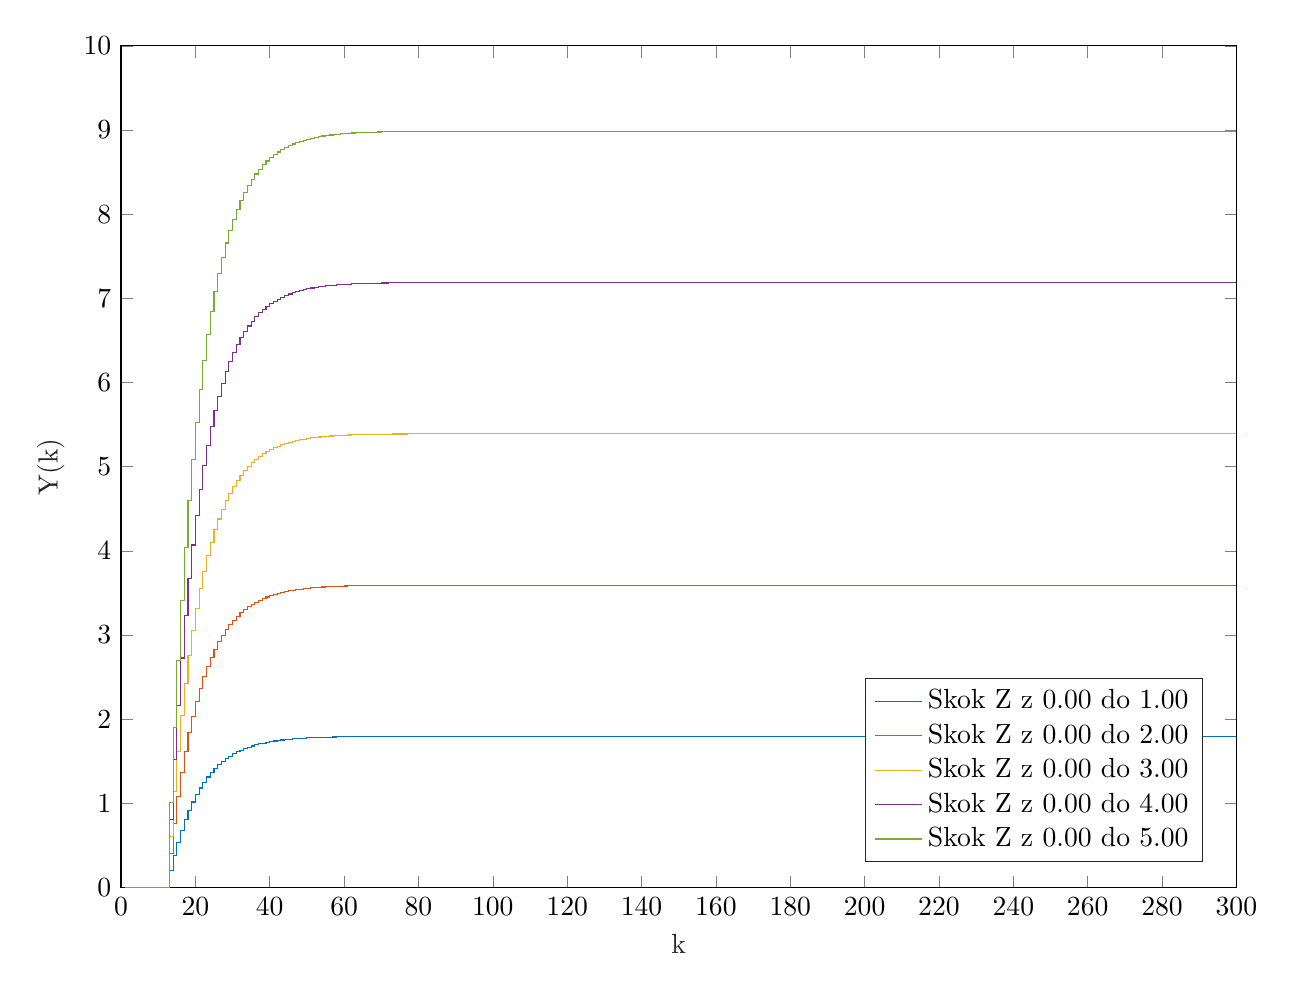
\begin{tikzpicture}

\begin{axis}[%
width=5.577in,
height=4.209in,
at={(0.768in,0.433in)},
scale only axis,
xmin=0,
xmax=300,
xlabel style={font=\color{white!15!black}},
xlabel={k},
ymin=0,
ymax=10,
ylabel style={font=\color{white!15!black}},
ylabel={Y(k)},
axis background/.style={fill=white},
legend style={at={(0.97,0.03)}, anchor=south east, legend cell align=left, align=left, draw=white!15!black}
]
\addplot[const plot, color=mycolor1] table[row sep=crcr] {%
1	0\\
2	0\\
3	0\\
4	0\\
5	0\\
6	0\\
7	0\\
8	0\\
9	0\\
10	0\\
11	0\\
12	0\\
13	0.20202\\
14	0.381363772\\
15	0.5405745884792\\
16	0.681910601930065\\
17	0.807376801662065\\
18	0.918753389257166\\
19	1.01762097400741\\
20	1.10538294469291\\
21	1.18328533412576\\
22	1.25243445742761\\
23	1.31381257352359\\
24	1.36829179137883\\
25	1.41664641767974\\
26	1.45956392062001\\
27	1.49765466487875\\
28	1.53146055549941\\
29	1.56146271294626\\
30	1.58808828791264\\
31	1.61171651228869\\
32	1.63268407189206\\
33	1.6512898769727\\
34	1.66779929798444\\
35	1.68244792655289\\
36	1.69544491485312\\
37	1.70697594064711\\
38	1.71720583993623\\
39	1.7262809444819\\
40	1.73433115727287\\
41	1.74147179531066\\
42	1.7478052257929\\
43	1.75342231885168\\
44	1.75840373740865\\
45	1.7628210824046\\
46	1.76673790961448\\
47	1.77021063244259\\
48	1.77328932347903\\
49	1.77601842616608\\
50	1.77843738665143\\
51	1.78058121477559\\
52	1.78248098213803\\
53	1.7841642642963\\
54	1.78565553336142\\
55	1.78697650655121\\
56	1.78814645563942\\
57	1.78918248168534\\
58	1.79009975893699\\
59	1.7909117513645\\
60	1.791630404893\\
61	1.79226631806014\\
62	1.7928288935179\\
63	1.7933264725271\\
64	1.79376645435222\\
65	1.79415540225022\\
66	1.79449913755705\\
67	1.79480282320733\\
68	1.7950710378724\\
69	1.79530784176955\\
70	1.79551683507687\\
71	1.79570120978355\\
72	1.79586379571225\\
73	1.79600710136771\\
74	1.79613335019233\\
75	1.79624451274432\\
76	1.79634233525612\\
77	1.79642836497965\\
78	1.79650397267911\\
79	1.79657037259177\\
80	1.79662864014108\\
81	1.7966797276547\\
82	1.79672447831156\\
83	1.79676363851692\\
84	1.79679786888231\\
85	1.79682775396694\\
86	1.79685381091999\\
87	1.79687649714742\\
88	1.79689621711284\\
89	1.79691332837016\\
90	1.79692814691417\\
91	1.79694095192608\\
92	1.79695198998197\\
93	1.79696147878477\\
94	1.79696961047339\\
95	1.79697655455666\\
96	1.79698246051441\\
97	1.79698746010321\\
98	1.79699166940006\\
99	1.79699519061374\\
100	1.79699811368989\\
101	1.79700051773321\\
102	1.79700247226746\\
103	1.79700403835162\\
104	1.79700526956837\\
105	1.79700621289954\\
106	1.79700690950111\\
107	1.79700739538939\\
108	1.79700770204824\\
109	1.79700785696642\\
110	1.797007884113\\
111	1.79700780435784\\
112	1.79700763584335\\
113	1.79700739431327\\
114	1.79700709340309\\
115	1.79700674489673\\
116	1.79700635895323\\
117	1.79700594430688\\
118	1.79700550844388\\
119	1.79700505775816\\
120	1.79700459768881\\
121	1.79700413284126\\
122	1.79700366709395\\
123	1.79700320369234\\
124	1.79700274533158\\
125	1.79700229422931\\
126	1.79700185218951\\
127	1.7970014206587\\
128	1.79700100077522\\
129	1.79700059341239\\
130	1.79700019921639\\
131	1.79699981863939\\
132	1.7969994519685\\
133	1.79699909935105\\
134	1.79699876081664\\
135	1.79699843629634\\
136	1.79699812563939\\
137	1.79699782862767\\
138	1.79699754498826\\
139	1.79699727440427\\
140	1.7969970165242\\
141	1.79699677096999\\
142	1.79699653734388\\
143	1.79699631523434\\
144	1.79699610422104\\
145	1.79699590387911\\
146	1.79699571378272\\
147	1.79699553350805\\
148	1.7969953626358\\
149	1.79699520075323\\
150	1.7969950474558\\
151	1.79699490234855\\
152	1.79699476504709\\
153	1.79699463517849\\
154	1.7969945123818\\
155	1.79699439630853\\
156	1.79699428662288\\
157	1.7969941830019\\
158	1.79699408513551\\
159	1.79699399272646\\
160	1.79699390549016\\
161	1.79699382315454\\
162	1.79699374545974\\
163	1.79699367215784\\
164	1.79699360301259\\
165	1.79699353779898\\
166	1.79699347630295\\
167	1.79699341832097\\
168	1.79699336365969\\
169	1.79699331213552\\
170	1.79699326357426\\
171	1.79699321781069\\
172	1.79699317468824\\
173	1.79699313405853\\
174	1.79699309578107\\
175	1.79699305972288\\
176	1.79699302575812\\
177	1.79699299376777\\
178	1.79699296363927\\
179	1.79699293526624\\
180	1.79699290854814\\
181	1.79699288339001\\
182	1.79699285970213\\
183	1.79699283739981\\
184	1.7969928164031\\
185	1.79699279663651\\
186	1.79699277802883\\
187	1.79699276051287\\
188	1.79699274402526\\
189	1.79699272850622\\
190	1.79699271389937\\
191	1.79699270015157\\
192	1.79699268721271\\
193	1.79699267503556\\
194	1.79699266357561\\
195	1.79699265279091\\
196	1.79699264264193\\
197	1.79699263309143\\
198	1.79699262410431\\
199	1.79699261564753\\
200	1.79699260768995\\
201	1.79699260020224\\
202	1.79699259315678\\
203	1.79699258652757\\
204	1.79699258029012\\
205	1.79699257442135\\
206	1.79699256889957\\
207	1.79699256370431\\
208	1.79699255881634\\
209	1.79699255421754\\
210	1.79699254989084\\
211	1.79699254582019\\
212	1.79699254199048\\
213	1.79699253838747\\
214	1.79699253499778\\
215	1.79699253180881\\
216	1.7969925288087\\
217	1.79699252598627\\
218	1.79699252333103\\
219	1.79699252083309\\
220	1.79699251848315\\
221	1.79699251627244\\
222	1.79699251419274\\
223	1.79699251223629\\
224	1.79699251039579\\
225	1.79699250866438\\
226	1.7969925070356\\
227	1.79699250550338\\
228	1.796992504062\\
229	1.79699250270607\\
230	1.79699250143053\\
231	1.79699250023063\\
232	1.79699249910187\\
233	1.79699249804005\\
234	1.7969924970412\\
235	1.79699249610159\\
236	1.7969924952177\\
237	1.79699249438624\\
238	1.79699249360409\\
239	1.79699249286833\\
240	1.79699249217621\\
241	1.79699249152515\\
242	1.79699249091271\\
243	1.7969924903366\\
244	1.79699248979466\\
245	1.79699248928488\\
246	1.79699248880533\\
247	1.79699248835424\\
248	1.79699248792991\\
249	1.79699248753075\\
250	1.79699248715528\\
251	1.79699248680208\\
252	1.79699248646984\\
253	1.79699248615731\\
254	1.79699248586332\\
255	1.79699248558678\\
256	1.79699248532664\\
257	1.79699248508194\\
258	1.79699248485176\\
259	1.79699248463524\\
260	1.79699248443157\\
261	1.79699248423998\\
262	1.79699248405976\\
263	1.79699248389023\\
264	1.79699248373076\\
265	1.79699248358076\\
266	1.79699248343965\\
267	1.79699248330692\\
268	1.79699248318207\\
269	1.79699248306463\\
270	1.79699248295415\\
271	1.79699248285023\\
272	1.79699248275248\\
273	1.79699248266053\\
274	1.79699248257403\\
275	1.79699248249267\\
276	1.79699248241613\\
277	1.79699248234414\\
278	1.79699248227642\\
279	1.79699248221272\\
280	1.7969924821528\\
281	1.79699248209644\\
282	1.79699248204342\\
283	1.79699248199354\\
284	1.79699248194663\\
285	1.7969924819025\\
286	1.79699248186099\\
287	1.79699248182194\\
288	1.79699248178521\\
289	1.79699248175066\\
290	1.79699248171816\\
291	1.79699248168759\\
292	1.79699248165883\\
293	1.79699248163178\\
294	1.79699248160634\\
295	1.7969924815824\\
296	1.79699248155989\\
297	1.79699248153871\\
298	1.79699248151878\\
299	1.79699248150005\\
300	1.79699248148242\\
};
\addlegendentry{Skok Z z 0.00 do 1.00}

\addplot[const plot, color=mycolor2] table[row sep=crcr] {%
1	0\\
2	0\\
3	0\\
4	0\\
5	0\\
6	0\\
7	0\\
8	0\\
9	0\\
10	0\\
11	0\\
12	0\\
13	0.40404\\
14	0.762727544\\
15	1.0811491769584\\
16	1.36382120386013\\
17	1.61475360332413\\
18	1.83750677851433\\
19	2.03524194801483\\
20	2.21076588938582\\
21	2.36657066825152\\
22	2.50486891485523\\
23	2.62762514704718\\
24	2.73658358275765\\
25	2.83329283535948\\
26	2.91912784124002\\
27	2.9953093297575\\
28	3.06292111099883\\
29	3.12292542589251\\
30	3.17617657582527\\
31	3.22343302457737\\
32	3.26536814378413\\
33	3.3025797539454\\
34	3.33559859596887\\
35	3.36489585310578\\
36	3.39088982970624\\
37	3.41395188129422\\
38	3.43441167987247\\
39	3.4525618889638\\
40	3.46866231454573\\
41	3.48294359062131\\
42	3.4956104515858\\
43	3.50684463770335\\
44	3.51680747481731\\
45	3.5256421648092\\
46	3.53347581922895\\
47	3.54042126488518\\
48	3.54657864695805\\
49	3.55203685233215\\
50	3.55687477330286\\
51	3.56116242955118\\
52	3.56496196427607\\
53	3.5683285285926\\
54	3.57131106672284\\
55	3.57395301310242\\
56	3.57629291127883\\
57	3.57836496337067\\
58	3.58019951787397\\
59	3.58182350272899\\
60	3.583260809786\\
61	3.58453263612028\\
62	3.5856577870358\\
63	3.58665294505419\\
64	3.58753290870444\\
65	3.58831080450043\\
66	3.58899827511411\\
67	3.58960564641467\\
68	3.5901420757448\\
69	3.5906156835391\\
70	3.59103367015375\\
71	3.59140241956711\\
72	3.5917275914245\\
73	3.59201420273541\\
74	3.59226670038466\\
75	3.59248902548864\\
76	3.59268467051224\\
77	3.59285672995929\\
78	3.59300794535821\\
79	3.59314074518353\\
80	3.59325728028216\\
81	3.59335945530941\\
82	3.59344895662311\\
83	3.59352727703384\\
84	3.59359573776463\\
85	3.59365550793388\\
86	3.59370762183999\\
87	3.59375299429483\\
88	3.59379243422568\\
89	3.59382665674032\\
90	3.59385629382835\\
91	3.59388190385216\\
92	3.59390397996394\\
93	3.59392295756954\\
94	3.59393922094678\\
95	3.59395310911333\\
96	3.59396492102883\\
97	3.59397492020641\\
98	3.59398333880011\\
99	3.59399038122748\\
100	3.59399622737978\\
101	3.59400103546641\\
102	3.59400494453492\\
103	3.59400807670323\\
104	3.59401053913674\\
105	3.59401242579907\\
106	3.59401381900222\\
107	3.59401479077878\\
108	3.59401540409647\\
109	3.59401571393284\\
110	3.59401576822601\\
111	3.59401560871567\\
112	3.59401527168671\\
113	3.59401478862655\\
114	3.59401418680618\\
115	3.59401348979346\\
116	3.59401271790646\\
117	3.59401188861377\\
118	3.59401101688776\\
119	3.59401011551631\\
120	3.59400919537762\\
121	3.59400826568252\\
122	3.5940073341879\\
123	3.59400640738467\\
124	3.59400549066316\\
125	3.59400458845862\\
126	3.59400370437902\\
127	3.59400284131741\\
128	3.59400200155044\\
129	3.59400118682477\\
130	3.59400039843277\\
131	3.59399963727877\\
132	3.593998903937\\
133	3.59399819870209\\
134	3.59399752163327\\
135	3.59399687259268\\
136	3.59399625127878\\
137	3.59399565725534\\
138	3.59399508997652\\
139	3.59399454880854\\
140	3.5939940330484\\
141	3.59399354193998\\
142	3.59399307468777\\
143	3.59399263046869\\
144	3.59399220844208\\
145	3.59399180775822\\
146	3.59399142756543\\
147	3.59399106701609\\
148	3.5939907252716\\
149	3.59399040150646\\
150	3.59399009491161\\
151	3.5939898046971\\
152	3.59398953009419\\
153	3.59398927035698\\
154	3.59398902476361\\
155	3.59398879261706\\
156	3.59398857324576\\
157	3.59398836600379\\
158	3.59398817027102\\
159	3.59398798545291\\
160	3.59398781098033\\
161	3.59398764630908\\
162	3.59398749091947\\
163	3.59398734431568\\
164	3.59398720602517\\
165	3.59398707559795\\
166	3.59398695260589\\
167	3.59398683664194\\
168	3.59398672731939\\
169	3.59398662427105\\
170	3.59398652714852\\
171	3.59398643562139\\
172	3.59398634937647\\
173	3.59398626811705\\
174	3.59398619156214\\
175	3.59398611944576\\
176	3.59398605151625\\
177	3.59398598753553\\
178	3.59398592727853\\
179	3.59398587053247\\
180	3.59398581709628\\
181	3.59398576678001\\
182	3.59398571940426\\
183	3.59398567479963\\
184	3.59398563280619\\
185	3.59398559327301\\
186	3.59398555605766\\
187	3.59398552102575\\
188	3.59398548805053\\
189	3.59398545701244\\
190	3.59398542779874\\
191	3.59398540030314\\
192	3.59398537442542\\
193	3.59398535007112\\
194	3.59398532715123\\
195	3.59398530558183\\
196	3.59398528528387\\
197	3.59398526618286\\
198	3.59398524820863\\
199	3.59398523129506\\
200	3.59398521537989\\
201	3.59398520040447\\
202	3.59398518631356\\
203	3.59398517305515\\
204	3.59398516058024\\
205	3.59398514884271\\
206	3.59398513779914\\
207	3.59398512740863\\
208	3.59398511763269\\
209	3.59398510843508\\
210	3.59398509978168\\
211	3.59398509164038\\
212	3.59398508398095\\
213	3.59398507677494\\
214	3.59398506999557\\
215	3.59398506361763\\
216	3.59398505761739\\
217	3.59398505197254\\
218	3.59398504666206\\
219	3.59398504166618\\
220	3.59398503696629\\
221	3.59398503254488\\
222	3.59398502838548\\
223	3.59398502447258\\
224	3.59398502079158\\
225	3.59398501732876\\
226	3.59398501407121\\
227	3.59398501100676\\
228	3.59398500812399\\
229	3.59398500541213\\
230	3.59398500286106\\
231	3.59398500046125\\
232	3.59398499820375\\
233	3.59398499608011\\
234	3.59398499408241\\
235	3.59398499220318\\
236	3.5939849904354\\
237	3.59398498877247\\
238	3.59398498720818\\
239	3.59398498573666\\
240	3.59398498435243\\
241	3.5939849830503\\
242	3.59398498182542\\
243	3.5939849806732\\
244	3.59398497958933\\
245	3.59398497856976\\
246	3.59398497761067\\
247	3.59398497670848\\
248	3.59398497585982\\
249	3.5939849750615\\
250	3.59398497431055\\
251	3.59398497360416\\
252	3.59398497293967\\
253	3.59398497231461\\
254	3.59398497172664\\
255	3.59398497117355\\
256	3.59398497065328\\
257	3.59398497016389\\
258	3.59398496970353\\
259	3.59398496927048\\
260	3.59398496886313\\
261	3.59398496847995\\
262	3.59398496811951\\
263	3.59398496778046\\
264	3.59398496746153\\
265	3.59398496716152\\
266	3.59398496687931\\
267	3.59398496661385\\
268	3.59398496636414\\
269	3.59398496612925\\
270	3.5939849659083\\
271	3.59398496570046\\
272	3.59398496550496\\
273	3.59398496532105\\
274	3.59398496514806\\
275	3.59398496498534\\
276	3.59398496483227\\
277	3.59398496468829\\
278	3.59398496455285\\
279	3.59398496442544\\
280	3.5939849643056\\
281	3.59398496419287\\
282	3.59398496408683\\
283	3.59398496398709\\
284	3.59398496389326\\
285	3.593984963805\\
286	3.59398496372198\\
287	3.59398496364388\\
288	3.59398496357042\\
289	3.59398496350132\\
290	3.59398496343632\\
291	3.59398496337518\\
292	3.59398496331766\\
293	3.59398496326356\\
294	3.59398496321267\\
295	3.5939849631648\\
296	3.59398496311977\\
297	3.59398496307741\\
298	3.59398496303757\\
299	3.59398496300009\\
300	3.59398496296484\\
};
\addlegendentry{Skok Z z 0.00 do 2.00}

\addplot[const plot, color=mycolor3] table[row sep=crcr] {%
1	0\\
2	0\\
3	0\\
4	0\\
5	0\\
6	0\\
7	0\\
8	0\\
9	0\\
10	0\\
11	0\\
12	0\\
13	0.60606\\
14	1.144091316\\
15	1.6217237654376\\
16	2.04573180579019\\
17	2.42213040498619\\
18	2.7562601677715\\
19	3.05286292202224\\
20	3.31614883407872\\
21	3.54985600237727\\
22	3.75730337228283\\
23	3.94143772057077\\
24	4.10487537413647\\
25	4.24993925303922\\
26	4.37869176186003\\
27	4.49296399463624\\
28	4.59438166649824\\
29	4.68438813883876\\
30	4.7642648637379\\
31	4.83514953686605\\
32	4.89805221567618\\
33	4.95386963091809\\
34	5.00339789395329\\
35	5.04734377965865\\
36	5.08633474455933\\
37	5.1209278219413\\
38	5.15161751980868\\
39	5.17884283344568\\
40	5.20299347181857\\
41	5.22441538593193\\
42	5.24341567737867\\
43	5.260266956555\\
44	5.27521121222593\\
45	5.28846324721377\\
46	5.30021372884339\\
47	5.31063189732773\\
48	5.31986797043704\\
49	5.32805527849818\\
50	5.33531215995424\\
51	5.34174364432672\\
52	5.34744294641406\\
53	5.35249279288886\\
54	5.35696660008422\\
55	5.36092951965359\\
56	5.3644393669182\\
57	5.36754744505597\\
58	5.37029927681091\\
59	5.37273525409344\\
60	5.37489121467895\\
61	5.37679895418037\\
62	5.37848668055364\\
63	5.37997941758123\\
64	5.38129936305661\\
65	5.3824662067506\\
66	5.38349741267111\\
67	5.38440846962195\\
68	5.38521311361715\\
69	5.38592352530859\\
70	5.38655050523056\\
71	5.3871036293506\\
72	5.38759138713669\\
73	5.38802130410305\\
74	5.38840005057693\\
75	5.38873353823289\\
76	5.38902700576829\\
77	5.38928509493887\\
78	5.38951191803725\\
79	5.38971111777523\\
80	5.38988592042316\\
81	5.39003918296404\\
82	5.39017343493459\\
83	5.39029091555068\\
84	5.39039360664686\\
85	5.39048326190074\\
86	5.3905614327599\\
87	5.39062949144216\\
88	5.39068865133843\\
89	5.39073998511039\\
90	5.39078444074244\\
91	5.39082285577817\\
92	5.39085596994583\\
93	5.39088443635424\\
94	5.3909088314201\\
95	5.39092966366992\\
96	5.39094738154318\\
97	5.39096238030955\\
98	5.39097500820011\\
99	5.39098557184116\\
100	5.39099434106961\\
101	5.39100155319956\\
102	5.39100741680232\\
103	5.3910121150548\\
104	5.39101580870506\\
105	5.39101863869855\\
106	5.39102072850327\\
107	5.39102218616811\\
108	5.39102310614466\\
109	5.3910235708992\\
110	5.39102365233896\\
111	5.39102341307346\\
112	5.39102290753001\\
113	5.39102218293977\\
114	5.39102128020922\\
115	5.39102023469014\\
116	5.39101907685963\\
117	5.39101783292059\\
118	5.39101652533158\\
119	5.3910151732744\\
120	5.39101379306637\\
121	5.39101239852372\\
122	5.39101100128179\\
123	5.39100961107694\\
124	5.39100823599468\\
125	5.39100688268786\\
126	5.39100555656846\\
127	5.39100426197605\\
128	5.39100300232561\\
129	5.3910017802371\\
130	5.3910005976491\\
131	5.39099945591811\\
132	5.39099835590544\\
133	5.39099729805309\\
134	5.39099628244986\\
135	5.39099530888897\\
136	5.39099437691813\\
137	5.39099348588297\\
138	5.39099263496474\\
139	5.39099182321277\\
140	5.39099104957257\\
141	5.39099031290994\\
142	5.39098961203162\\
143	5.390988945703\\
144	5.39098831266309\\
145	5.3909877116373\\
146	5.39098714134812\\
147	5.39098660052411\\
148	5.39098608790738\\
149	5.39098560225967\\
150	5.39098514236739\\
151	5.39098470704562\\
152	5.39098429514126\\
153	5.39098390553546\\
154	5.3909835371454\\
155	5.39098318892558\\
156	5.39098285986863\\
157	5.39098254900568\\
158	5.39098225540651\\
159	5.39098197817935\\
160	5.39098171647048\\
161	5.39098146946361\\
162	5.39098123637919\\
163	5.3909810164735\\
164	5.39098080903773\\
165	5.3909806133969\\
166	5.39098042890881\\
167	5.39098025496288\\
168	5.39098009097904\\
169	5.39097993640653\\
170	5.39097979072274\\
171	5.39097965343205\\
172	5.39097952406467\\
173	5.39097940217554\\
174	5.39097928734317\\
175	5.39097917916861\\
176	5.39097907727433\\
177	5.39097898130326\\
178	5.39097889091775\\
179	5.39097880579865\\
180	5.39097872564437\\
181	5.39097865016997\\
182	5.39097857910634\\
183	5.39097851219939\\
184	5.39097844920923\\
185	5.39097838990946\\
186	5.39097833408643\\
187	5.39097828153857\\
188	5.39097823207574\\
189	5.3909781855186\\
190	5.39097814169806\\
191	5.39097810045465\\
192	5.39097806163808\\
193	5.39097802510664\\
194	5.3909779907268\\
195	5.3909779583727\\
196	5.39097792792576\\
197	5.39097789927425\\
198	5.3909778723129\\
199	5.39097784694255\\
200	5.3909778230698\\
201	5.39097780060667\\
202	5.39097777947031\\
203	5.39097775958268\\
204	5.39097774087032\\
205	5.39097772326403\\
206	5.39097770669867\\
207	5.3909776911129\\
208	5.39097767644899\\
209	5.39097766265258\\
210	5.39097764967248\\
211	5.39097763746053\\
212	5.39097762597139\\
213	5.39097761516238\\
214	5.39097760499332\\
215	5.3909775954264\\
216	5.39097758642605\\
217	5.39097757795877\\
218	5.39097756999305\\
219	5.39097756249923\\
220	5.3909775554494\\
221	5.39097754881728\\
222	5.39097754257817\\
223	5.39097753670881\\
224	5.39097753118731\\
225	5.39097752599309\\
226	5.39097752110675\\
227	5.39097751651008\\
228	5.39097751218592\\
229	5.39097750811813\\
230	5.39097750429152\\
231	5.39097750069181\\
232	5.39097749730555\\
233	5.39097749412009\\
234	5.39097749112353\\
235	5.39097748830469\\
236	5.39097748565302\\
237	5.39097748315863\\
238	5.39097748081218\\
239	5.39097747860491\\
240	5.39097747652856\\
241	5.39097747457537\\
242	5.39097747273805\\
243	5.39097747100971\\
244	5.39097746938391\\
245	5.39097746785455\\
246	5.39097746641592\\
247	5.39097746506264\\
248	5.39097746378965\\
249	5.39097746259218\\
250	5.39097746146575\\
251	5.39097746040616\\
252	5.39097745940943\\
253	5.39097745847184\\
254	5.39097745758988\\
255	5.39097745676025\\
256	5.39097745597985\\
257	5.39097745524575\\
258	5.39097745455521\\
259	5.39097745390564\\
260	5.39097745329462\\
261	5.39097745271985\\
262	5.39097745217919\\
263	5.39097745167061\\
264	5.39097745119221\\
265	5.39097745074219\\
266	5.39097745031888\\
267	5.3909774499207\\
268	5.39097744954614\\
269	5.39097744919381\\
270	5.39097744886238\\
271	5.39097744855062\\
272	5.39097744825737\\
273	5.39097744798151\\
274	5.39097744772203\\
275	5.39097744747794\\
276	5.39097744724834\\
277	5.39097744703236\\
278	5.3909774468292\\
279	5.3909774466381\\
280	5.39097744645833\\
281	5.39097744628924\\
282	5.39097744613018\\
283	5.39097744598056\\
284	5.39097744583982\\
285	5.39097744570743\\
286	5.39097744558289\\
287	5.39097744546575\\
288	5.39097744535556\\
289	5.39097744525191\\
290	5.39097744515442\\
291	5.3909774450627\\
292	5.39097744497643\\
293	5.39097744489528\\
294	5.39097744481894\\
295	5.39097744474714\\
296	5.3909774446796\\
297	5.39097744461606\\
298	5.39097744455629\\
299	5.39097744450007\\
300	5.39097744444719\\
};
\addlegendentry{Skok Z z 0.00 do 3.00}

\addplot[const plot, color=mycolor4] table[row sep=crcr] {%
1	0\\
2	0\\
3	0\\
4	0\\
5	0\\
6	0\\
7	0\\
8	0\\
9	0\\
10	0\\
11	0\\
12	0\\
13	0.80808\\
14	1.525455088\\
15	2.1622983539168\\
16	2.72764240772026\\
17	3.22950720664826\\
18	3.67501355702866\\
19	4.07048389602965\\
20	4.42153177877163\\
21	4.73314133650304\\
22	5.00973782971045\\
23	5.25525029409437\\
24	5.47316716551531\\
25	5.66658567071897\\
26	5.83825568248005\\
27	5.99061865951499\\
28	6.12584222199766\\
29	6.24585085178502\\
30	6.35235315165055\\
31	6.44686604915475\\
32	6.53073628756826\\
33	6.60515950789081\\
34	6.67119719193775\\
35	6.72979170621157\\
36	6.78177965941247\\
37	6.82790376258843\\
38	6.86882335974494\\
39	6.90512377792761\\
40	6.93732462909147\\
41	6.96588718124262\\
42	6.99122090317161\\
43	7.01368927540671\\
44	7.03361494963462\\
45	7.05128432961841\\
46	7.06695163845791\\
47	7.08084252977036\\
48	7.09315729391611\\
49	7.1040737046643\\
50	7.11374954660572\\
51	7.12232485910235\\
52	7.12992392855214\\
53	7.1366570571852\\
54	7.14262213344568\\
55	7.14790602620484\\
56	7.15258582255766\\
57	7.15672992674135\\
58	7.16039903574795\\
59	7.16364700545798\\
60	7.16652161957199\\
61	7.16906527224057\\
62	7.17131557407159\\
63	7.17330589010838\\
64	7.17506581740889\\
65	7.17662160900087\\
66	7.17799655022821\\
67	7.17921129282934\\
68	7.18028415148961\\
69	7.1812313670782\\
70	7.18206734030749\\
71	7.18280483913422\\
72	7.183455182849\\
73	7.18402840547083\\
74	7.18453340076932\\
75	7.18497805097728\\
76	7.18536934102448\\
77	7.18571345991858\\
78	7.18601589071643\\
79	7.18628149036706\\
80	7.18651456056432\\
81	7.18671891061882\\
82	7.18689791324623\\
83	7.18705455406768\\
84	7.18719147552925\\
85	7.18731101586776\\
86	7.18741524367998\\
87	7.18750598858966\\
88	7.18758486845136\\
89	7.18765331348063\\
90	7.18771258765669\\
91	7.18776380770433\\
92	7.18780795992788\\
93	7.18784591513908\\
94	7.18787844189356\\
95	7.18790621822665\\
96	7.18792984205766\\
97	7.18794984041282\\
98	7.18796667760023\\
99	7.18798076245497\\
100	7.18799245475956\\
101	7.18800207093283\\
102	7.18800988906984\\
103	7.18801615340647\\
104	7.18802107827348\\
105	7.18802485159814\\
106	7.18802763800443\\
107	7.18802958155756\\
108	7.18803080819295\\
109	7.18803142786568\\
110	7.18803153645201\\
111	7.18803121743135\\
112	7.18803054337342\\
113	7.1880295772531\\
114	7.18802837361237\\
115	7.18802697958693\\
116	7.18802543581292\\
117	7.18802377722753\\
118	7.18802203377552\\
119	7.18802023103262\\
120	7.18801839075525\\
121	7.18801653136505\\
122	7.18801466837581\\
123	7.18801281476934\\
124	7.18801098132633\\
125	7.18800917691723\\
126	7.18800740875803\\
127	7.18800568263482\\
128	7.18800400310088\\
129	7.18800237364954\\
130	7.18800079686554\\
131	7.18799927455755\\
132	7.18799780787399\\
133	7.18799639740418\\
134	7.18799504326654\\
135	7.18799374518535\\
136	7.18799250255756\\
137	7.18799131451068\\
138	7.18799017995304\\
139	7.18798909761707\\
140	7.18798806609681\\
141	7.18798708387996\\
142	7.18798614937554\\
143	7.18798526093737\\
144	7.18798441688416\\
145	7.18798361551644\\
146	7.18798285513086\\
147	7.18798213403219\\
148	7.18798145054321\\
149	7.18798080301292\\
150	7.18798018982322\\
151	7.18797960939419\\
152	7.18797906018838\\
153	7.18797854071397\\
154	7.18797804952722\\
155	7.18797758523413\\
156	7.18797714649152\\
157	7.18797673200759\\
158	7.18797634054203\\
159	7.18797597090582\\
160	7.18797562196066\\
161	7.18797529261817\\
162	7.18797498183894\\
163	7.18797468863137\\
164	7.18797441205034\\
165	7.1879741511959\\
166	7.18797390521178\\
167	7.18797367328389\\
168	7.18797345463877\\
169	7.18797324854209\\
170	7.18797305429704\\
171	7.18797287124278\\
172	7.18797269875294\\
173	7.1879725362341\\
174	7.18797238312428\\
175	7.18797223889153\\
176	7.18797210303249\\
177	7.18797197507107\\
178	7.18797185455707\\
179	7.18797174106494\\
180	7.18797163419256\\
181	7.18797153356003\\
182	7.18797143880853\\
183	7.18797134959926\\
184	7.18797126561238\\
185	7.18797118654602\\
186	7.18797111211532\\
187	7.1879710420515\\
188	7.18797097610105\\
189	7.18797091402487\\
190	7.18797085559748\\
191	7.18797080060627\\
192	7.18797074885083\\
193	7.18797070014225\\
194	7.18797065430246\\
195	7.18797061116366\\
196	7.18797057056774\\
197	7.18797053236572\\
198	7.18797049641725\\
199	7.18797046259012\\
200	7.18797043075979\\
201	7.18797040080895\\
202	7.18797037262713\\
203	7.18797034611029\\
204	7.18797032116047\\
205	7.18797029768542\\
206	7.18797027559827\\
207	7.18797025481725\\
208	7.18797023526537\\
209	7.18797021687015\\
210	7.18797019956336\\
211	7.18797018328076\\
212	7.1879701679619\\
213	7.18797015354988\\
214	7.18797013999114\\
215	7.18797012723525\\
216	7.18797011523478\\
217	7.18797010394508\\
218	7.18797009332412\\
219	7.18797008333236\\
220	7.18797007393258\\
221	7.18797006508977\\
222	7.18797005677096\\
223	7.18797004894515\\
224	7.18797004158316\\
225	7.18797003465752\\
226	7.18797002814242\\
227	7.18797002201353\\
228	7.18797001624798\\
229	7.18797001082426\\
230	7.18797000572212\\
231	7.1879700009225\\
232	7.18796999640749\\
233	7.18796999216022\\
234	7.18796998816482\\
235	7.18796998440636\\
236	7.18796998087081\\
237	7.18796997754495\\
238	7.18796997441635\\
239	7.18796997147332\\
240	7.18796996870485\\
241	7.18796996610061\\
242	7.18796996365084\\
243	7.18796996134639\\
244	7.18796995917865\\
245	7.18796995713951\\
246	7.18796995522134\\
247	7.18796995341696\\
248	7.18796995171964\\
249	7.18796995012301\\
250	7.18796994862111\\
251	7.18796994720831\\
252	7.18796994587935\\
253	7.18796994462923\\
254	7.18796994345328\\
255	7.18796994234711\\
256	7.18796994130657\\
257	7.18796994032777\\
258	7.18796993940705\\
259	7.18796993854096\\
260	7.18796993772626\\
261	7.18796993695991\\
262	7.18796993623903\\
263	7.18796993556092\\
264	7.18796993492305\\
265	7.18796993432303\\
266	7.18796993375862\\
267	7.1879699332277\\
268	7.18796993272828\\
269	7.18796993225851\\
270	7.1879699318166\\
271	7.18796993140093\\
272	7.18796993100991\\
273	7.18796993064211\\
274	7.18796993029613\\
275	7.18796992997068\\
276	7.18796992966454\\
277	7.18796992937657\\
278	7.18796992910569\\
279	7.18796992885089\\
280	7.1879699286112\\
281	7.18796992838574\\
282	7.18796992817366\\
283	7.18796992797417\\
284	7.18796992778652\\
285	7.18796992761\\
286	7.18796992744395\\
287	7.18796992728776\\
288	7.18796992714084\\
289	7.18796992700264\\
290	7.18796992687264\\
291	7.18796992675035\\
292	7.18796992663532\\
293	7.18796992652712\\
294	7.18796992642534\\
295	7.1879699263296\\
296	7.18796992623954\\
297	7.18796992615483\\
298	7.18796992607514\\
299	7.18796992600018\\
300	7.18796992592967\\
};
\addlegendentry{Skok Z z 0.00 do 4.00}

\addplot[const plot, color=mycolor5] table[row sep=crcr] {%
1	0\\
2	0\\
3	0\\
4	0\\
5	0\\
6	0\\
7	0\\
8	0\\
9	0\\
10	0\\
11	0\\
12	0\\
13	1.0101\\
14	1.90681886\\
15	2.702872942396\\
16	3.40955300965033\\
17	4.03688400831033\\
18	4.59376694628583\\
19	5.08810487003707\\
20	5.52691472346454\\
21	5.9164266706288\\
22	6.26217228713806\\
23	6.56906286761795\\
24	6.84145895689412\\
25	7.08323208839869\\
26	7.29781960310004\\
27	7.48827332439372\\
28	7.65730277749704\\
29	7.80731356473124\\
30	7.94044143956314\\
31	8.05858256144339\\
32	8.16342035946026\\
33	8.25644938486344\\
34	8.33899648992211\\
35	8.41223963276438\\
36	8.4772245742655\\
37	8.53487970323544\\
38	8.58602919968106\\
39	8.63140472240939\\
40	8.67165578636421\\
41	8.70735897655314\\
42	8.73902612896437\\
43	8.76711159425823\\
44	8.79201868704311\\
45	8.81410541202285\\
46	8.83368954807222\\
47	8.85105316221278\\
48	8.86644661739496\\
49	8.88009213083021\\
50	8.89218693325697\\
51	8.90290607387777\\
52	8.91240491069001\\
53	8.92082132148134\\
54	8.92827766680695\\
55	8.9348825327559\\
56	8.94073227819693\\
57	8.94591240842655\\
58	8.9504987946848\\
59	8.95455875682235\\
60	8.95815202446487\\
61	8.96133159030059\\
62	8.96414446758939\\
63	8.96663236263538\\
64	8.96883227176102\\
65	8.97077701125101\\
66	8.9724956877852\\
67	8.97401411603662\\
68	8.97535518936197\\
69	8.97653920884771\\
70	8.97758417538435\\
71	8.97850604891776\\
72	8.97931897856124\\
73	8.98003550683853\\
74	8.98066675096166\\
75	8.98122256372161\\
76	8.9817116762806\\
77	8.98214182489824\\
78	8.98251986339555\\
79	8.98285186295884\\
80	8.98314320070541\\
81	8.98339863827354\\
82	8.9836223915578\\
83	8.98381819258462\\
84	8.98398934441158\\
85	8.98413876983471\\
86	8.98426905459998\\
87	8.98438248573708\\
88	8.9844810855642\\
89	8.9845666418508\\
90	8.98464073457087\\
91	8.98470475963041\\
92	8.98475994990986\\
93	8.98480739392386\\
94	8.98484805236697\\
95	8.98488277278333\\
96	8.98491230257209\\
97	8.98493730051605\\
98	8.98495834700031\\
99	8.98497595306874\\
100	8.98499056844949\\
101	8.98500258866607\\
102	8.98501236133734\\
103	8.98502019175813\\
104	8.9850263478419\\
105	8.98503106449771\\
106	8.98503454750557\\
107	8.98503697694698\\
108	8.98503851024121\\
109	8.98503928483212\\
110	8.98503942056504\\
111	8.9850390217892\\
112	8.98503817921679\\
113	8.98503697156639\\
114	8.98503546701548\\
115	8.98503372448367\\
116	8.98503179476617\\
117	8.98502972153443\\
118	8.98502754221941\\
119	8.98502528879079\\
120	8.98502298844407\\
121	8.98502066420633\\
122	8.98501833546978\\
123	8.9850160184617\\
124	8.98501372665794\\
125	8.98501147114657\\
126	8.98500926094758\\
127	8.98500710329357\\
128	8.98500500387615\\
129	8.98500296706198\\
130	8.98500099608199\\
131	8.984999093197\\
132	8.98499725984255\\
133	8.9849954967553\\
134	8.98499380408325\\
135	8.98499218148177\\
136	8.98499062819703\\
137	8.98498914313844\\
138	8.98498772494138\\
139	8.98498637202142\\
140	8.98498508262109\\
141	8.98498385485003\\
142	8.9849826867195\\
143	8.98498157617179\\
144	8.98498052110527\\
145	8.98497951939562\\
146	8.98497856891365\\
147	8.98497766754031\\
148	8.98497681317909\\
149	8.98497600376623\\
150	8.98497523727911\\
151	8.98497451174283\\
152	8.98497382523556\\
153	8.98497317589255\\
154	8.98497256190911\\
155	8.98497198154275\\
156	8.9849714331145\\
157	8.98497091500958\\
158	8.98497042567764\\
159	8.98496996363237\\
160	8.98496952745091\\
161	8.9849691157728\\
162	8.98496872729877\\
163	8.9849683607893\\
164	8.98496801506302\\
165	8.98496768899498\\
166	8.98496738151483\\
167	8.98496709160496\\
168	8.98496681829857\\
169	8.98496656067772\\
170	8.98496631787141\\
171	8.98496608905359\\
172	8.9849658734413\\
173	8.98496567029275\\
174	8.98496547890548\\
175	8.98496529861454\\
176	8.98496512879074\\
177	8.98496496883896\\
178	8.98496481819646\\
179	8.9849646763313\\
180	8.98496454274083\\
181	8.98496441695017\\
182	8.98496429851079\\
183	8.98496418699921\\
184	8.98496408201562\\
185	8.98496398318267\\
186	8.98496389014428\\
187	8.98496380256451\\
188	8.98496372012646\\
189	8.98496364253123\\
190	8.98496356949699\\
191	8.98496350075799\\
192	8.9849634360637\\
193	8.98496337517797\\
194	8.98496331787823\\
195	8.98496326395473\\
196	8.98496321320983\\
197	8.98496316545731\\
198	8.98496312052172\\
199	8.98496307823781\\
200	8.98496303844988\\
201	8.98496300101133\\
202	8.98496296578405\\
203	8.98496293263801\\
204	8.98496290145073\\
205	8.98496287210691\\
206	8.98496284449797\\
207	8.9849628185217\\
208	8.98496279408185\\
209	8.98496277108782\\
210	8.98496274945432\\
211	8.98496272910107\\
212	8.9849627099525\\
213	8.98496269193747\\
214	8.98496267498903\\
215	8.98496265904417\\
216	8.98496264404358\\
217	8.98496262993145\\
218	8.98496261665525\\
219	8.98496260416555\\
220	8.98496259241583\\
221	8.98496258136231\\
222	8.98496257096379\\
223	8.98496256118153\\
224	8.98496255197904\\
225	8.98496254332199\\
226	8.98496253517811\\
227	8.984962527517\\
228	8.98496252031007\\
229	8.98496251353042\\
230	8.98496250715274\\
231	8.98496250115321\\
232	8.98496249550944\\
233	8.98496249020035\\
234	8.98496248520609\\
235	8.98496248050802\\
236	8.98496247608857\\
237	8.98496247193124\\
238	8.98496246802049\\
239	8.9849624643417\\
240	8.98496246088112\\
241	8.98496245762581\\
242	8.9849624545636\\
243	8.98496245168304\\
244	8.98496244897337\\
245	8.98496244642444\\
246	8.98496244402672\\
247	8.98496244177125\\
248	8.98496243964959\\
249	8.9849624376538\\
250	8.98496243577642\\
251	8.98496243401043\\
252	8.98496243234921\\
253	8.98496243078656\\
254	8.98496242931662\\
255	8.9849624279339\\
256	8.98496242663323\\
257	8.98496242540973\\
258	8.98496242425882\\
259	8.98496242317622\\
260	8.98496242215785\\
261	8.9849624211999\\
262	8.9849624202988\\
263	8.98496241945117\\
264	8.98496241865384\\
265	8.98496241790382\\
266	8.9849624171983\\
267	8.98496241653465\\
268	8.98496241591038\\
269	8.98496241532316\\
270	8.98496241477078\\
271	8.98496241425118\\
272	8.98496241376242\\
273	8.98496241330266\\
274	8.98496241287019\\
275	8.98496241246337\\
276	8.9849624120807\\
277	8.98496241172074\\
278	8.98496241138214\\
279	8.98496241106363\\
280	8.98496241076403\\
281	8.9849624104822\\
282	8.9849624102171\\
283	8.98496240996773\\
284	8.98496240973316\\
285	8.98496240951251\\
286	8.98496240930496\\
287	8.98496240910972\\
288	8.98496240892607\\
289	8.98496240875332\\
290	8.98496240859082\\
291	8.98496240843796\\
292	8.98496240829417\\
293	8.98496240815892\\
294	8.98496240803169\\
295	8.98496240791202\\
296	8.98496240779944\\
297	8.98496240769355\\
298	8.98496240759394\\
299	8.98496240750024\\
300	8.9849624074121\\
};
\addlegendentry{Skok Z z 0.00 do 5.00}

\end{axis}
\end{tikzpicture}%
\caption{Wykresy odpowiedzi skokowych}
\end{figure}

Jak i w przypadku toru U-Y tutaj widzimy proporcjonalność.

\section{Charakterystyka statyczna}

Otrzymana charakterystyka statyczna z rozdzielczościa 50/1 (dla skoków 0,02, 0,04, 0,06 ...)


\begin{figure}[H]
\centering
% This file was created by matlab2tikz.
%
%The latest updates can be retrieved from
%  http://www.mathworks.com/matlabcentral/fileexchange/22022-matlab2tikz-matlab2tikz
%where you can also make suggestions and rate matlab2tikz.
%
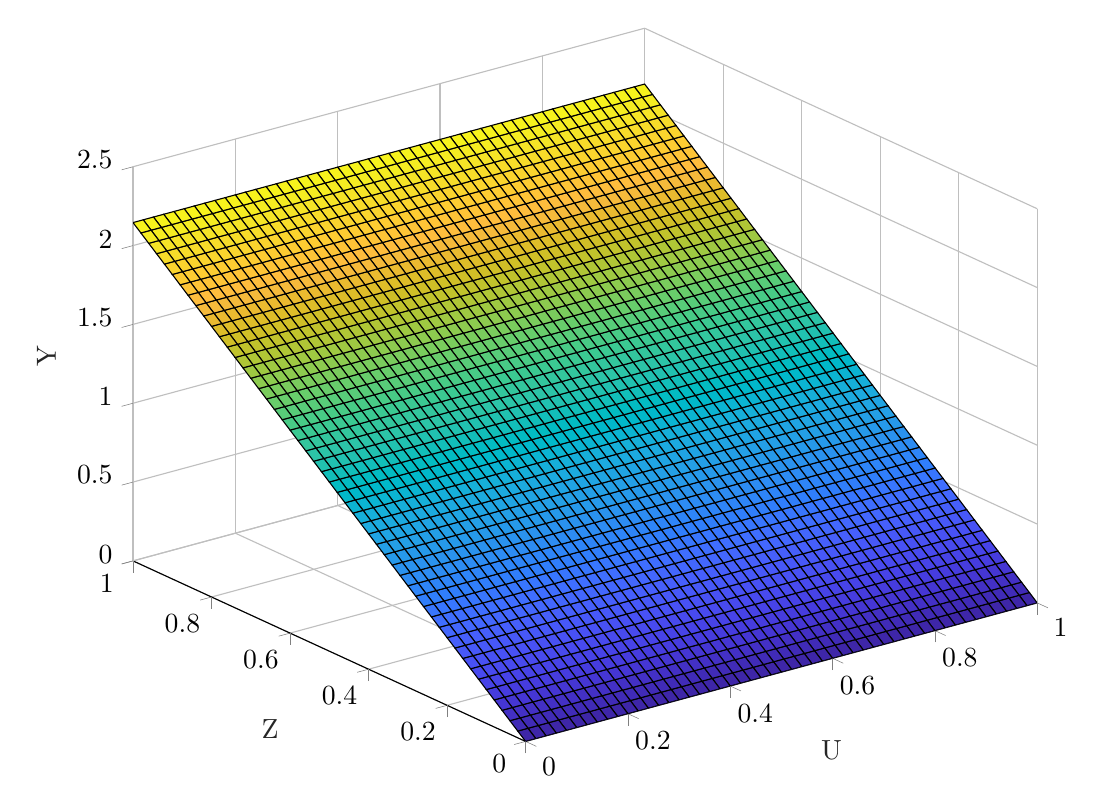
\begin{tikzpicture}

\begin{axis}[%
width=4.521in,
height=3.566in,
at={(0.758in,0.481in)},
scale only axis,
xmin=0,
xmax=1,
tick align=outside,
xlabel style={font=\color{white!15!black}},
xlabel={U},
ymin=0,
ymax=1,
ylabel style={font=\color{white!15!black}},
ylabel={Z},
zmin=0,
zmax=2.5,
zlabel style={font=\color{white!15!black}},
zlabel={Y},
view={-37.5}{30},
axis background/.style={fill=white},
axis x line*=bottom,
axis y line*=left,
axis z line*=left,
xmajorgrids,
ymajorgrids,
zmajorgrids
]

\addplot3[%
surf,
shader=flat corner, draw=black, z buffer=sort, colormap={mymap}{[1pt] rgb(0pt)=(0.2422,0.1504,0.6603); rgb(1pt)=(0.2444,0.1534,0.6728); rgb(2pt)=(0.2464,0.1569,0.6847); rgb(3pt)=(0.2484,0.1607,0.6961); rgb(4pt)=(0.2503,0.1648,0.7071); rgb(5pt)=(0.2522,0.1689,0.7179); rgb(6pt)=(0.254,0.1732,0.7286); rgb(7pt)=(0.2558,0.1773,0.7393); rgb(8pt)=(0.2576,0.1814,0.7501); rgb(9pt)=(0.2594,0.1854,0.761); rgb(11pt)=(0.2628,0.1932,0.7828); rgb(12pt)=(0.2645,0.1972,0.7937); rgb(13pt)=(0.2661,0.2011,0.8043); rgb(14pt)=(0.2676,0.2052,0.8148); rgb(15pt)=(0.2691,0.2094,0.8249); rgb(16pt)=(0.2704,0.2138,0.8346); rgb(17pt)=(0.2717,0.2184,0.8439); rgb(18pt)=(0.2729,0.2231,0.8528); rgb(19pt)=(0.274,0.228,0.8612); rgb(20pt)=(0.2749,0.233,0.8692); rgb(21pt)=(0.2758,0.2382,0.8767); rgb(22pt)=(0.2766,0.2435,0.884); rgb(23pt)=(0.2774,0.2489,0.8908); rgb(24pt)=(0.2781,0.2543,0.8973); rgb(25pt)=(0.2788,0.2598,0.9035); rgb(26pt)=(0.2794,0.2653,0.9094); rgb(27pt)=(0.2798,0.2708,0.915); rgb(28pt)=(0.2802,0.2764,0.9204); rgb(29pt)=(0.2806,0.2819,0.9255); rgb(30pt)=(0.2809,0.2875,0.9305); rgb(31pt)=(0.2811,0.293,0.9352); rgb(32pt)=(0.2813,0.2985,0.9397); rgb(33pt)=(0.2814,0.304,0.9441); rgb(34pt)=(0.2814,0.3095,0.9483); rgb(35pt)=(0.2813,0.315,0.9524); rgb(36pt)=(0.2811,0.3204,0.9563); rgb(37pt)=(0.2809,0.3259,0.96); rgb(38pt)=(0.2807,0.3313,0.9636); rgb(39pt)=(0.2803,0.3367,0.967); rgb(40pt)=(0.2798,0.3421,0.9702); rgb(41pt)=(0.2791,0.3475,0.9733); rgb(42pt)=(0.2784,0.3529,0.9763); rgb(43pt)=(0.2776,0.3583,0.9791); rgb(44pt)=(0.2766,0.3638,0.9817); rgb(45pt)=(0.2754,0.3693,0.984); rgb(46pt)=(0.2741,0.3748,0.9862); rgb(47pt)=(0.2726,0.3804,0.9881); rgb(48pt)=(0.271,0.386,0.9898); rgb(49pt)=(0.2691,0.3916,0.9912); rgb(50pt)=(0.267,0.3973,0.9924); rgb(51pt)=(0.2647,0.403,0.9935); rgb(52pt)=(0.2621,0.4088,0.9946); rgb(53pt)=(0.2591,0.4145,0.9955); rgb(54pt)=(0.2556,0.4203,0.9965); rgb(55pt)=(0.2517,0.4261,0.9974); rgb(56pt)=(0.2473,0.4319,0.9983); rgb(57pt)=(0.2424,0.4378,0.9991); rgb(58pt)=(0.2369,0.4437,0.9996); rgb(59pt)=(0.2311,0.4497,0.9995); rgb(60pt)=(0.225,0.4559,0.9985); rgb(61pt)=(0.2189,0.462,0.9968); rgb(62pt)=(0.2128,0.4682,0.9948); rgb(63pt)=(0.2066,0.4743,0.9926); rgb(64pt)=(0.2006,0.4803,0.9906); rgb(65pt)=(0.195,0.4861,0.9887); rgb(66pt)=(0.1903,0.4919,0.9867); rgb(67pt)=(0.1869,0.4975,0.9844); rgb(68pt)=(0.1847,0.503,0.9819); rgb(69pt)=(0.1831,0.5084,0.9793); rgb(70pt)=(0.1818,0.5138,0.9766); rgb(71pt)=(0.1806,0.5191,0.9738); rgb(72pt)=(0.1795,0.5244,0.9709); rgb(73pt)=(0.1785,0.5296,0.9677); rgb(74pt)=(0.1778,0.5349,0.9641); rgb(75pt)=(0.1773,0.5401,0.9602); rgb(76pt)=(0.1768,0.5452,0.956); rgb(77pt)=(0.1764,0.5504,0.9516); rgb(78pt)=(0.1755,0.5554,0.9473); rgb(79pt)=(0.174,0.5605,0.9432); rgb(80pt)=(0.1716,0.5655,0.9393); rgb(81pt)=(0.1686,0.5705,0.9357); rgb(82pt)=(0.1649,0.5755,0.9323); rgb(83pt)=(0.161,0.5805,0.9289); rgb(84pt)=(0.1573,0.5854,0.9254); rgb(85pt)=(0.154,0.5902,0.9218); rgb(86pt)=(0.1513,0.595,0.9182); rgb(87pt)=(0.1492,0.5997,0.9147); rgb(88pt)=(0.1475,0.6043,0.9113); rgb(89pt)=(0.1461,0.6089,0.908); rgb(90pt)=(0.1446,0.6135,0.905); rgb(91pt)=(0.1429,0.618,0.9022); rgb(92pt)=(0.1408,0.6226,0.8998); rgb(93pt)=(0.1383,0.6272,0.8975); rgb(94pt)=(0.1354,0.6317,0.8953); rgb(95pt)=(0.1321,0.6363,0.8932); rgb(96pt)=(0.1288,0.6408,0.891); rgb(97pt)=(0.1253,0.6453,0.8887); rgb(98pt)=(0.1219,0.6497,0.8862); rgb(99pt)=(0.1185,0.6541,0.8834); rgb(100pt)=(0.1152,0.6584,0.8804); rgb(101pt)=(0.1119,0.6627,0.877); rgb(102pt)=(0.1085,0.6669,0.8734); rgb(103pt)=(0.1048,0.671,0.8695); rgb(104pt)=(0.1009,0.675,0.8653); rgb(105pt)=(0.0964,0.6789,0.8609); rgb(106pt)=(0.0914,0.6828,0.8562); rgb(107pt)=(0.0855,0.6865,0.8513); rgb(108pt)=(0.0789,0.6902,0.8462); rgb(109pt)=(0.0713,0.6938,0.8409); rgb(110pt)=(0.0628,0.6972,0.8355); rgb(111pt)=(0.0535,0.7006,0.8299); rgb(112pt)=(0.0433,0.7039,0.8242); rgb(113pt)=(0.0328,0.7071,0.8183); rgb(114pt)=(0.0234,0.7103,0.8124); rgb(115pt)=(0.0155,0.7133,0.8064); rgb(116pt)=(0.0091,0.7163,0.8003); rgb(117pt)=(0.0046,0.7192,0.7941); rgb(118pt)=(0.0019,0.722,0.7878); rgb(119pt)=(0.0009,0.7248,0.7815); rgb(120pt)=(0.0018,0.7275,0.7752); rgb(121pt)=(0.0046,0.7301,0.7688); rgb(122pt)=(0.0094,0.7327,0.7623); rgb(123pt)=(0.0162,0.7352,0.7558); rgb(124pt)=(0.0253,0.7376,0.7492); rgb(125pt)=(0.0369,0.74,0.7426); rgb(126pt)=(0.0504,0.7423,0.7359); rgb(127pt)=(0.0638,0.7446,0.7292); rgb(128pt)=(0.077,0.7468,0.7224); rgb(129pt)=(0.0899,0.7489,0.7156); rgb(130pt)=(0.1023,0.751,0.7088); rgb(131pt)=(0.1141,0.7531,0.7019); rgb(132pt)=(0.1252,0.7552,0.695); rgb(133pt)=(0.1354,0.7572,0.6881); rgb(134pt)=(0.1448,0.7593,0.6812); rgb(135pt)=(0.1532,0.7614,0.6741); rgb(136pt)=(0.1609,0.7635,0.6671); rgb(137pt)=(0.1678,0.7656,0.6599); rgb(138pt)=(0.1741,0.7678,0.6527); rgb(139pt)=(0.1799,0.7699,0.6454); rgb(140pt)=(0.1853,0.7721,0.6379); rgb(141pt)=(0.1905,0.7743,0.6303); rgb(142pt)=(0.1954,0.7765,0.6225); rgb(143pt)=(0.2003,0.7787,0.6146); rgb(144pt)=(0.2061,0.7808,0.6065); rgb(145pt)=(0.2118,0.7828,0.5983); rgb(146pt)=(0.2178,0.7849,0.5899); rgb(147pt)=(0.2244,0.7869,0.5813); rgb(148pt)=(0.2318,0.7887,0.5725); rgb(149pt)=(0.2401,0.7905,0.5636); rgb(150pt)=(0.2491,0.7922,0.5546); rgb(151pt)=(0.2589,0.7937,0.5454); rgb(152pt)=(0.2695,0.7951,0.536); rgb(153pt)=(0.2809,0.7964,0.5266); rgb(154pt)=(0.2929,0.7975,0.517); rgb(155pt)=(0.3052,0.7985,0.5074); rgb(156pt)=(0.3176,0.7994,0.4975); rgb(157pt)=(0.3301,0.8002,0.4876); rgb(158pt)=(0.3424,0.8009,0.4774); rgb(159pt)=(0.3548,0.8016,0.4669); rgb(160pt)=(0.3671,0.8021,0.4563); rgb(161pt)=(0.3795,0.8026,0.4454); rgb(162pt)=(0.3921,0.8029,0.4344); rgb(163pt)=(0.405,0.8031,0.4233); rgb(164pt)=(0.4184,0.803,0.4122); rgb(165pt)=(0.4322,0.8028,0.4013); rgb(166pt)=(0.4463,0.8024,0.3904); rgb(167pt)=(0.4608,0.8018,0.3797); rgb(168pt)=(0.4753,0.8011,0.3691); rgb(169pt)=(0.4899,0.8002,0.3586); rgb(170pt)=(0.5044,0.7993,0.348); rgb(171pt)=(0.5187,0.7982,0.3374); rgb(172pt)=(0.5329,0.797,0.3267); rgb(173pt)=(0.547,0.7957,0.3159); rgb(175pt)=(0.5748,0.7929,0.2941); rgb(176pt)=(0.5886,0.7913,0.2833); rgb(177pt)=(0.6024,0.7896,0.2726); rgb(178pt)=(0.6161,0.7878,0.2622); rgb(179pt)=(0.6297,0.7859,0.2521); rgb(180pt)=(0.6433,0.7839,0.2423); rgb(181pt)=(0.6567,0.7818,0.2329); rgb(182pt)=(0.6701,0.7796,0.2239); rgb(183pt)=(0.6833,0.7773,0.2155); rgb(184pt)=(0.6963,0.775,0.2075); rgb(185pt)=(0.7091,0.7727,0.1998); rgb(186pt)=(0.7218,0.7703,0.1924); rgb(187pt)=(0.7344,0.7679,0.1852); rgb(188pt)=(0.7468,0.7654,0.1782); rgb(189pt)=(0.759,0.7629,0.1717); rgb(190pt)=(0.771,0.7604,0.1658); rgb(191pt)=(0.7829,0.7579,0.1608); rgb(192pt)=(0.7945,0.7554,0.157); rgb(193pt)=(0.806,0.7529,0.1546); rgb(194pt)=(0.8172,0.7505,0.1535); rgb(195pt)=(0.8281,0.7481,0.1536); rgb(196pt)=(0.8389,0.7457,0.1546); rgb(197pt)=(0.8495,0.7435,0.1564); rgb(198pt)=(0.86,0.7413,0.1587); rgb(199pt)=(0.8703,0.7392,0.1615); rgb(200pt)=(0.8804,0.7372,0.165); rgb(201pt)=(0.8903,0.7353,0.1695); rgb(202pt)=(0.9,0.7336,0.1749); rgb(203pt)=(0.9093,0.7321,0.1815); rgb(204pt)=(0.9184,0.7308,0.189); rgb(205pt)=(0.9272,0.7298,0.1973); rgb(206pt)=(0.9357,0.729,0.2061); rgb(207pt)=(0.944,0.7285,0.2151); rgb(208pt)=(0.9523,0.7284,0.2237); rgb(209pt)=(0.9606,0.7285,0.2312); rgb(210pt)=(0.9689,0.7292,0.2373); rgb(211pt)=(0.977,0.7304,0.2418); rgb(212pt)=(0.9842,0.733,0.2446); rgb(213pt)=(0.99,0.7365,0.2429); rgb(214pt)=(0.9946,0.7407,0.2394); rgb(215pt)=(0.9966,0.7458,0.2351); rgb(216pt)=(0.9971,0.7513,0.2309); rgb(217pt)=(0.9972,0.7569,0.2267); rgb(218pt)=(0.9971,0.7626,0.2224); rgb(219pt)=(0.9969,0.7683,0.2181); rgb(220pt)=(0.9966,0.774,0.2138); rgb(221pt)=(0.9962,0.7798,0.2095); rgb(222pt)=(0.9957,0.7856,0.2053); rgb(223pt)=(0.9949,0.7915,0.2012); rgb(224pt)=(0.9938,0.7974,0.1974); rgb(225pt)=(0.9923,0.8034,0.1939); rgb(226pt)=(0.9906,0.8095,0.1906); rgb(227pt)=(0.9885,0.8156,0.1875); rgb(228pt)=(0.9861,0.8218,0.1846); rgb(229pt)=(0.9835,0.828,0.1817); rgb(230pt)=(0.9807,0.8342,0.1787); rgb(231pt)=(0.9778,0.8404,0.1757); rgb(232pt)=(0.9748,0.8467,0.1726); rgb(233pt)=(0.972,0.8529,0.1695); rgb(234pt)=(0.9694,0.8591,0.1665); rgb(235pt)=(0.9671,0.8654,0.1636); rgb(236pt)=(0.9651,0.8716,0.1608); rgb(237pt)=(0.9634,0.8778,0.1582); rgb(238pt)=(0.9619,0.884,0.1557); rgb(239pt)=(0.9608,0.8902,0.1532); rgb(240pt)=(0.9601,0.8963,0.1507); rgb(241pt)=(0.9596,0.9023,0.148); rgb(242pt)=(0.9595,0.9084,0.145); rgb(243pt)=(0.9597,0.9143,0.1418); rgb(244pt)=(0.9601,0.9203,0.1382); rgb(245pt)=(0.9608,0.9262,0.1344); rgb(246pt)=(0.9618,0.932,0.1304); rgb(247pt)=(0.9629,0.9379,0.1261); rgb(248pt)=(0.9642,0.9437,0.1216); rgb(249pt)=(0.9657,0.9494,0.1168); rgb(250pt)=(0.9674,0.9552,0.1116); rgb(251pt)=(0.9692,0.9609,0.1061); rgb(252pt)=(0.9711,0.9667,0.1001); rgb(253pt)=(0.973,0.9724,0.0938); rgb(254pt)=(0.9749,0.9782,0.0872); rgb(255pt)=(0.9769,0.9839,0.0805)}, mesh/rows=51]
table[row sep=crcr, point meta=\thisrow{c}] {%
%
x	y	z	c\\
0	0	0	0\\
0	0.02	0.0429172925253396	0.0429172925253396\\
0	0.04	0.0858345850506791	0.0858345850506791\\
0	0.06	0.128751877576017	0.128751877576017\\
0	0.08	0.171669170101358	0.171669170101358\\
0	0.1	0.214586462626696	0.214586462626696\\
0	0.12	0.257503755152033	0.257503755152033\\
0	0.14	0.300421047677378	0.300421047677378\\
0	0.16	0.343338340202716	0.343338340202716\\
0	0.18	0.386255632728053	0.386255632728053\\
0	0.2	0.429172925253391	0.429172925253391\\
0	0.22	0.472090217778728	0.472090217778728\\
0	0.24	0.515007510304066	0.515007510304066\\
0	0.26	0.557924802829403	0.557924802829403\\
0	0.28	0.600842095354757	0.600842095354757\\
0	0.3	0.643759387880079	0.643759387880079\\
0	0.32	0.686676680405433	0.686676680405433\\
0	0.34	0.729593972930751	0.729593972930751\\
0	0.36	0.772511265456106	0.772511265456106\\
0	0.38	0.815428557981429	0.815428557981429\\
0	0.4	0.858345850506782	0.858345850506782\\
0	0.42	0.901263143032101	0.901263143032101\\
0	0.44	0.944180435557456	0.944180435557456\\
0	0.46	0.987097728082777	0.987097728082777\\
0	0.48	1.03001502060813	1.03001502060813\\
0	0.5	1.07293231313349	1.07293231313349\\
0	0.52	1.11584960565881	1.11584960565881\\
0	0.54	1.15876689818416	1.15876689818416\\
0	0.56	1.20168419070951	1.20168419070951\\
0	0.58	1.2446014832348	1.2446014832348\\
0	0.6	1.28751877576016	1.28751877576016\\
0	0.62	1.33043606828551	1.33043606828551\\
0	0.64	1.37335336081087	1.37335336081087\\
0	0.66	1.41627065333616	1.41627065333616\\
0	0.68	1.4591879458615	1.4591879458615\\
0	0.7	1.50210523838686	1.50210523838686\\
0	0.72	1.54502253091221	1.54502253091221\\
0	0.74	1.58793982343753	1.58793982343753\\
0	0.76	1.63085711596286	1.63085711596286\\
0	0.78	1.67377440848821	1.67377440848821\\
0	0.8	1.71669170101356	1.71669170101356\\
0	0.82	1.75960899353892	1.75960899353892\\
0	0.84	1.8025262860642	1.8025262860642\\
0	0.86	1.84544357858955	1.84544357858955\\
0	0.88	1.88836087111491	1.88836087111491\\
0	0.9	1.93127816364027	1.93127816364027\\
0	0.92	1.97419545616555	1.97419545616555\\
0	0.94	2.0171127486909	2.0171127486909\\
0	0.96	2.06003004121627	2.06003004121627\\
0	0.98	2.10294733374162	2.10294733374162\\
0	1	2.14586462626697	2.14586462626697\\
0.02	0	0	0\\
0.02	0.02	0.0429172925253396	0.0429172925253396\\
0.02	0.04	0.0858345850506791	0.0858345850506791\\
0.02	0.06	0.128751877576017	0.128751877576017\\
0.02	0.08	0.171669170101358	0.171669170101358\\
0.02	0.1	0.214586462626696	0.214586462626696\\
0.02	0.12	0.257503755152033	0.257503755152033\\
0.02	0.14	0.300421047677378	0.300421047677378\\
0.02	0.16	0.343338340202716	0.343338340202716\\
0.02	0.18	0.386255632728053	0.386255632728053\\
0.02	0.2	0.429172925253391	0.429172925253391\\
0.02	0.22	0.472090217778728	0.472090217778728\\
0.02	0.24	0.515007510304066	0.515007510304066\\
0.02	0.26	0.557924802829403	0.557924802829403\\
0.02	0.28	0.600842095354757	0.600842095354757\\
0.02	0.3	0.643759387880079	0.643759387880079\\
0.02	0.32	0.686676680405433	0.686676680405433\\
0.02	0.34	0.729593972930751	0.729593972930751\\
0.02	0.36	0.772511265456106	0.772511265456106\\
0.02	0.38	0.815428557981429	0.815428557981429\\
0.02	0.4	0.858345850506782	0.858345850506782\\
0.02	0.42	0.901263143032101	0.901263143032101\\
0.02	0.44	0.944180435557456	0.944180435557456\\
0.02	0.46	0.987097728082777	0.987097728082777\\
0.02	0.48	1.03001502060813	1.03001502060813\\
0.02	0.5	1.07293231313349	1.07293231313349\\
0.02	0.52	1.11584960565881	1.11584960565881\\
0.02	0.54	1.15876689818416	1.15876689818416\\
0.02	0.56	1.20168419070951	1.20168419070951\\
0.02	0.58	1.2446014832348	1.2446014832348\\
0.02	0.6	1.28751877576016	1.28751877576016\\
0.02	0.62	1.33043606828551	1.33043606828551\\
0.02	0.64	1.37335336081087	1.37335336081087\\
0.02	0.66	1.41627065333616	1.41627065333616\\
0.02	0.68	1.4591879458615	1.4591879458615\\
0.02	0.7	1.50210523838686	1.50210523838686\\
0.02	0.72	1.54502253091221	1.54502253091221\\
0.02	0.74	1.58793982343753	1.58793982343753\\
0.02	0.76	1.63085711596286	1.63085711596286\\
0.02	0.78	1.67377440848821	1.67377440848821\\
0.02	0.8	1.71669170101356	1.71669170101356\\
0.02	0.82	1.75960899353892	1.75960899353892\\
0.02	0.84	1.8025262860642	1.8025262860642\\
0.02	0.86	1.84544357858955	1.84544357858955\\
0.02	0.88	1.88836087111491	1.88836087111491\\
0.02	0.9	1.93127816364027	1.93127816364027\\
0.02	0.92	1.97419545616555	1.97419545616555\\
0.02	0.94	2.0171127486909	2.0171127486909\\
0.02	0.96	2.06003004121627	2.06003004121627\\
0.02	0.98	2.10294733374162	2.10294733374162\\
0.02	1	2.14586462626697	2.14586462626697\\
0.04	0	0	0\\
0.04	0.02	0.0429172925253396	0.0429172925253396\\
0.04	0.04	0.0858345850506791	0.0858345850506791\\
0.04	0.06	0.128751877576017	0.128751877576017\\
0.04	0.08	0.171669170101358	0.171669170101358\\
0.04	0.1	0.214586462626696	0.214586462626696\\
0.04	0.12	0.257503755152033	0.257503755152033\\
0.04	0.14	0.300421047677378	0.300421047677378\\
0.04	0.16	0.343338340202716	0.343338340202716\\
0.04	0.18	0.386255632728053	0.386255632728053\\
0.04	0.2	0.429172925253391	0.429172925253391\\
0.04	0.22	0.472090217778728	0.472090217778728\\
0.04	0.24	0.515007510304066	0.515007510304066\\
0.04	0.26	0.557924802829403	0.557924802829403\\
0.04	0.28	0.600842095354757	0.600842095354757\\
0.04	0.3	0.643759387880079	0.643759387880079\\
0.04	0.32	0.686676680405433	0.686676680405433\\
0.04	0.34	0.729593972930751	0.729593972930751\\
0.04	0.36	0.772511265456106	0.772511265456106\\
0.04	0.38	0.815428557981429	0.815428557981429\\
0.04	0.4	0.858345850506782	0.858345850506782\\
0.04	0.42	0.901263143032101	0.901263143032101\\
0.04	0.44	0.944180435557456	0.944180435557456\\
0.04	0.46	0.987097728082777	0.987097728082777\\
0.04	0.48	1.03001502060813	1.03001502060813\\
0.04	0.5	1.07293231313349	1.07293231313349\\
0.04	0.52	1.11584960565881	1.11584960565881\\
0.04	0.54	1.15876689818416	1.15876689818416\\
0.04	0.56	1.20168419070951	1.20168419070951\\
0.04	0.58	1.2446014832348	1.2446014832348\\
0.04	0.6	1.28751877576016	1.28751877576016\\
0.04	0.62	1.33043606828551	1.33043606828551\\
0.04	0.64	1.37335336081087	1.37335336081087\\
0.04	0.66	1.41627065333616	1.41627065333616\\
0.04	0.68	1.4591879458615	1.4591879458615\\
0.04	0.7	1.50210523838686	1.50210523838686\\
0.04	0.72	1.54502253091221	1.54502253091221\\
0.04	0.74	1.58793982343753	1.58793982343753\\
0.04	0.76	1.63085711596286	1.63085711596286\\
0.04	0.78	1.67377440848821	1.67377440848821\\
0.04	0.8	1.71669170101356	1.71669170101356\\
0.04	0.82	1.75960899353892	1.75960899353892\\
0.04	0.84	1.8025262860642	1.8025262860642\\
0.04	0.86	1.84544357858955	1.84544357858955\\
0.04	0.88	1.88836087111491	1.88836087111491\\
0.04	0.9	1.93127816364027	1.93127816364027\\
0.04	0.92	1.97419545616555	1.97419545616555\\
0.04	0.94	2.0171127486909	2.0171127486909\\
0.04	0.96	2.06003004121627	2.06003004121627\\
0.04	0.98	2.10294733374162	2.10294733374162\\
0.04	1	2.14586462626697	2.14586462626697\\
0.06	0	0	0\\
0.06	0.02	0.0429172925253396	0.0429172925253396\\
0.06	0.04	0.0858345850506791	0.0858345850506791\\
0.06	0.06	0.128751877576017	0.128751877576017\\
0.06	0.08	0.171669170101358	0.171669170101358\\
0.06	0.1	0.214586462626696	0.214586462626696\\
0.06	0.12	0.257503755152033	0.257503755152033\\
0.06	0.14	0.300421047677378	0.300421047677378\\
0.06	0.16	0.343338340202716	0.343338340202716\\
0.06	0.18	0.386255632728053	0.386255632728053\\
0.06	0.2	0.429172925253391	0.429172925253391\\
0.06	0.22	0.472090217778728	0.472090217778728\\
0.06	0.24	0.515007510304066	0.515007510304066\\
0.06	0.26	0.557924802829403	0.557924802829403\\
0.06	0.28	0.600842095354757	0.600842095354757\\
0.06	0.3	0.643759387880079	0.643759387880079\\
0.06	0.32	0.686676680405433	0.686676680405433\\
0.06	0.34	0.729593972930751	0.729593972930751\\
0.06	0.36	0.772511265456106	0.772511265456106\\
0.06	0.38	0.815428557981429	0.815428557981429\\
0.06	0.4	0.858345850506782	0.858345850506782\\
0.06	0.42	0.901263143032101	0.901263143032101\\
0.06	0.44	0.944180435557456	0.944180435557456\\
0.06	0.46	0.987097728082777	0.987097728082777\\
0.06	0.48	1.03001502060813	1.03001502060813\\
0.06	0.5	1.07293231313349	1.07293231313349\\
0.06	0.52	1.11584960565881	1.11584960565881\\
0.06	0.54	1.15876689818416	1.15876689818416\\
0.06	0.56	1.20168419070951	1.20168419070951\\
0.06	0.58	1.2446014832348	1.2446014832348\\
0.06	0.6	1.28751877576016	1.28751877576016\\
0.06	0.62	1.33043606828551	1.33043606828551\\
0.06	0.64	1.37335336081087	1.37335336081087\\
0.06	0.66	1.41627065333616	1.41627065333616\\
0.06	0.68	1.4591879458615	1.4591879458615\\
0.06	0.7	1.50210523838686	1.50210523838686\\
0.06	0.72	1.54502253091221	1.54502253091221\\
0.06	0.74	1.58793982343753	1.58793982343753\\
0.06	0.76	1.63085711596286	1.63085711596286\\
0.06	0.78	1.67377440848821	1.67377440848821\\
0.06	0.8	1.71669170101356	1.71669170101356\\
0.06	0.82	1.75960899353892	1.75960899353892\\
0.06	0.84	1.8025262860642	1.8025262860642\\
0.06	0.86	1.84544357858955	1.84544357858955\\
0.06	0.88	1.88836087111491	1.88836087111491\\
0.06	0.9	1.93127816364027	1.93127816364027\\
0.06	0.92	1.97419545616555	1.97419545616555\\
0.06	0.94	2.0171127486909	2.0171127486909\\
0.06	0.96	2.06003004121627	2.06003004121627\\
0.06	0.98	2.10294733374162	2.10294733374162\\
0.06	1	2.14586462626697	2.14586462626697\\
0.08	0	0	0\\
0.08	0.02	0.0429172925253396	0.0429172925253396\\
0.08	0.04	0.0858345850506791	0.0858345850506791\\
0.08	0.06	0.128751877576017	0.128751877576017\\
0.08	0.08	0.171669170101358	0.171669170101358\\
0.08	0.1	0.214586462626696	0.214586462626696\\
0.08	0.12	0.257503755152033	0.257503755152033\\
0.08	0.14	0.300421047677378	0.300421047677378\\
0.08	0.16	0.343338340202716	0.343338340202716\\
0.08	0.18	0.386255632728053	0.386255632728053\\
0.08	0.2	0.429172925253391	0.429172925253391\\
0.08	0.22	0.472090217778728	0.472090217778728\\
0.08	0.24	0.515007510304066	0.515007510304066\\
0.08	0.26	0.557924802829403	0.557924802829403\\
0.08	0.28	0.600842095354757	0.600842095354757\\
0.08	0.3	0.643759387880079	0.643759387880079\\
0.08	0.32	0.686676680405433	0.686676680405433\\
0.08	0.34	0.729593972930751	0.729593972930751\\
0.08	0.36	0.772511265456106	0.772511265456106\\
0.08	0.38	0.815428557981429	0.815428557981429\\
0.08	0.4	0.858345850506782	0.858345850506782\\
0.08	0.42	0.901263143032101	0.901263143032101\\
0.08	0.44	0.944180435557456	0.944180435557456\\
0.08	0.46	0.987097728082777	0.987097728082777\\
0.08	0.48	1.03001502060813	1.03001502060813\\
0.08	0.5	1.07293231313349	1.07293231313349\\
0.08	0.52	1.11584960565881	1.11584960565881\\
0.08	0.54	1.15876689818416	1.15876689818416\\
0.08	0.56	1.20168419070951	1.20168419070951\\
0.08	0.58	1.2446014832348	1.2446014832348\\
0.08	0.6	1.28751877576016	1.28751877576016\\
0.08	0.62	1.33043606828551	1.33043606828551\\
0.08	0.64	1.37335336081087	1.37335336081087\\
0.08	0.66	1.41627065333616	1.41627065333616\\
0.08	0.68	1.4591879458615	1.4591879458615\\
0.08	0.7	1.50210523838686	1.50210523838686\\
0.08	0.72	1.54502253091221	1.54502253091221\\
0.08	0.74	1.58793982343753	1.58793982343753\\
0.08	0.76	1.63085711596286	1.63085711596286\\
0.08	0.78	1.67377440848821	1.67377440848821\\
0.08	0.8	1.71669170101356	1.71669170101356\\
0.08	0.82	1.75960899353892	1.75960899353892\\
0.08	0.84	1.8025262860642	1.8025262860642\\
0.08	0.86	1.84544357858955	1.84544357858955\\
0.08	0.88	1.88836087111491	1.88836087111491\\
0.08	0.9	1.93127816364027	1.93127816364027\\
0.08	0.92	1.97419545616555	1.97419545616555\\
0.08	0.94	2.0171127486909	2.0171127486909\\
0.08	0.96	2.06003004121627	2.06003004121627\\
0.08	0.98	2.10294733374162	2.10294733374162\\
0.08	1	2.14586462626697	2.14586462626697\\
0.1	0	0	0\\
0.1	0.02	0.0429172925253396	0.0429172925253396\\
0.1	0.04	0.0858345850506791	0.0858345850506791\\
0.1	0.06	0.128751877576017	0.128751877576017\\
0.1	0.08	0.171669170101358	0.171669170101358\\
0.1	0.1	0.214586462626696	0.214586462626696\\
0.1	0.12	0.257503755152033	0.257503755152033\\
0.1	0.14	0.300421047677378	0.300421047677378\\
0.1	0.16	0.343338340202716	0.343338340202716\\
0.1	0.18	0.386255632728053	0.386255632728053\\
0.1	0.2	0.429172925253391	0.429172925253391\\
0.1	0.22	0.472090217778728	0.472090217778728\\
0.1	0.24	0.515007510304066	0.515007510304066\\
0.1	0.26	0.557924802829403	0.557924802829403\\
0.1	0.28	0.600842095354757	0.600842095354757\\
0.1	0.3	0.643759387880079	0.643759387880079\\
0.1	0.32	0.686676680405433	0.686676680405433\\
0.1	0.34	0.729593972930751	0.729593972930751\\
0.1	0.36	0.772511265456106	0.772511265456106\\
0.1	0.38	0.815428557981429	0.815428557981429\\
0.1	0.4	0.858345850506782	0.858345850506782\\
0.1	0.42	0.901263143032101	0.901263143032101\\
0.1	0.44	0.944180435557456	0.944180435557456\\
0.1	0.46	0.987097728082777	0.987097728082777\\
0.1	0.48	1.03001502060813	1.03001502060813\\
0.1	0.5	1.07293231313349	1.07293231313349\\
0.1	0.52	1.11584960565881	1.11584960565881\\
0.1	0.54	1.15876689818416	1.15876689818416\\
0.1	0.56	1.20168419070951	1.20168419070951\\
0.1	0.58	1.2446014832348	1.2446014832348\\
0.1	0.6	1.28751877576016	1.28751877576016\\
0.1	0.62	1.33043606828551	1.33043606828551\\
0.1	0.64	1.37335336081087	1.37335336081087\\
0.1	0.66	1.41627065333616	1.41627065333616\\
0.1	0.68	1.4591879458615	1.4591879458615\\
0.1	0.7	1.50210523838686	1.50210523838686\\
0.1	0.72	1.54502253091221	1.54502253091221\\
0.1	0.74	1.58793982343753	1.58793982343753\\
0.1	0.76	1.63085711596286	1.63085711596286\\
0.1	0.78	1.67377440848821	1.67377440848821\\
0.1	0.8	1.71669170101356	1.71669170101356\\
0.1	0.82	1.75960899353892	1.75960899353892\\
0.1	0.84	1.8025262860642	1.8025262860642\\
0.1	0.86	1.84544357858955	1.84544357858955\\
0.1	0.88	1.88836087111491	1.88836087111491\\
0.1	0.9	1.93127816364027	1.93127816364027\\
0.1	0.92	1.97419545616555	1.97419545616555\\
0.1	0.94	2.0171127486909	2.0171127486909\\
0.1	0.96	2.06003004121627	2.06003004121627\\
0.1	0.98	2.10294733374162	2.10294733374162\\
0.1	1	2.14586462626697	2.14586462626697\\
0.12	0	0	0\\
0.12	0.02	0.0429172925253396	0.0429172925253396\\
0.12	0.04	0.0858345850506791	0.0858345850506791\\
0.12	0.06	0.128751877576017	0.128751877576017\\
0.12	0.08	0.171669170101358	0.171669170101358\\
0.12	0.1	0.214586462626696	0.214586462626696\\
0.12	0.12	0.257503755152033	0.257503755152033\\
0.12	0.14	0.300421047677378	0.300421047677378\\
0.12	0.16	0.343338340202716	0.343338340202716\\
0.12	0.18	0.386255632728053	0.386255632728053\\
0.12	0.2	0.429172925253391	0.429172925253391\\
0.12	0.22	0.472090217778728	0.472090217778728\\
0.12	0.24	0.515007510304066	0.515007510304066\\
0.12	0.26	0.557924802829403	0.557924802829403\\
0.12	0.28	0.600842095354757	0.600842095354757\\
0.12	0.3	0.643759387880079	0.643759387880079\\
0.12	0.32	0.686676680405433	0.686676680405433\\
0.12	0.34	0.729593972930751	0.729593972930751\\
0.12	0.36	0.772511265456106	0.772511265456106\\
0.12	0.38	0.815428557981429	0.815428557981429\\
0.12	0.4	0.858345850506782	0.858345850506782\\
0.12	0.42	0.901263143032101	0.901263143032101\\
0.12	0.44	0.944180435557456	0.944180435557456\\
0.12	0.46	0.987097728082777	0.987097728082777\\
0.12	0.48	1.03001502060813	1.03001502060813\\
0.12	0.5	1.07293231313349	1.07293231313349\\
0.12	0.52	1.11584960565881	1.11584960565881\\
0.12	0.54	1.15876689818416	1.15876689818416\\
0.12	0.56	1.20168419070951	1.20168419070951\\
0.12	0.58	1.2446014832348	1.2446014832348\\
0.12	0.6	1.28751877576016	1.28751877576016\\
0.12	0.62	1.33043606828551	1.33043606828551\\
0.12	0.64	1.37335336081087	1.37335336081087\\
0.12	0.66	1.41627065333616	1.41627065333616\\
0.12	0.68	1.4591879458615	1.4591879458615\\
0.12	0.7	1.50210523838686	1.50210523838686\\
0.12	0.72	1.54502253091221	1.54502253091221\\
0.12	0.74	1.58793982343753	1.58793982343753\\
0.12	0.76	1.63085711596286	1.63085711596286\\
0.12	0.78	1.67377440848821	1.67377440848821\\
0.12	0.8	1.71669170101356	1.71669170101356\\
0.12	0.82	1.75960899353892	1.75960899353892\\
0.12	0.84	1.8025262860642	1.8025262860642\\
0.12	0.86	1.84544357858955	1.84544357858955\\
0.12	0.88	1.88836087111491	1.88836087111491\\
0.12	0.9	1.93127816364027	1.93127816364027\\
0.12	0.92	1.97419545616555	1.97419545616555\\
0.12	0.94	2.0171127486909	2.0171127486909\\
0.12	0.96	2.06003004121627	2.06003004121627\\
0.12	0.98	2.10294733374162	2.10294733374162\\
0.12	1	2.14586462626697	2.14586462626697\\
0.14	0	0	0\\
0.14	0.02	0.0429172925253396	0.0429172925253396\\
0.14	0.04	0.0858345850506791	0.0858345850506791\\
0.14	0.06	0.128751877576017	0.128751877576017\\
0.14	0.08	0.171669170101358	0.171669170101358\\
0.14	0.1	0.214586462626696	0.214586462626696\\
0.14	0.12	0.257503755152033	0.257503755152033\\
0.14	0.14	0.300421047677378	0.300421047677378\\
0.14	0.16	0.343338340202716	0.343338340202716\\
0.14	0.18	0.386255632728053	0.386255632728053\\
0.14	0.2	0.429172925253391	0.429172925253391\\
0.14	0.22	0.472090217778728	0.472090217778728\\
0.14	0.24	0.515007510304066	0.515007510304066\\
0.14	0.26	0.557924802829403	0.557924802829403\\
0.14	0.28	0.600842095354757	0.600842095354757\\
0.14	0.3	0.643759387880079	0.643759387880079\\
0.14	0.32	0.686676680405433	0.686676680405433\\
0.14	0.34	0.729593972930751	0.729593972930751\\
0.14	0.36	0.772511265456106	0.772511265456106\\
0.14	0.38	0.815428557981429	0.815428557981429\\
0.14	0.4	0.858345850506782	0.858345850506782\\
0.14	0.42	0.901263143032101	0.901263143032101\\
0.14	0.44	0.944180435557456	0.944180435557456\\
0.14	0.46	0.987097728082777	0.987097728082777\\
0.14	0.48	1.03001502060813	1.03001502060813\\
0.14	0.5	1.07293231313349	1.07293231313349\\
0.14	0.52	1.11584960565881	1.11584960565881\\
0.14	0.54	1.15876689818416	1.15876689818416\\
0.14	0.56	1.20168419070951	1.20168419070951\\
0.14	0.58	1.2446014832348	1.2446014832348\\
0.14	0.6	1.28751877576016	1.28751877576016\\
0.14	0.62	1.33043606828551	1.33043606828551\\
0.14	0.64	1.37335336081087	1.37335336081087\\
0.14	0.66	1.41627065333616	1.41627065333616\\
0.14	0.68	1.4591879458615	1.4591879458615\\
0.14	0.7	1.50210523838686	1.50210523838686\\
0.14	0.72	1.54502253091221	1.54502253091221\\
0.14	0.74	1.58793982343753	1.58793982343753\\
0.14	0.76	1.63085711596286	1.63085711596286\\
0.14	0.78	1.67377440848821	1.67377440848821\\
0.14	0.8	1.71669170101356	1.71669170101356\\
0.14	0.82	1.75960899353892	1.75960899353892\\
0.14	0.84	1.8025262860642	1.8025262860642\\
0.14	0.86	1.84544357858955	1.84544357858955\\
0.14	0.88	1.88836087111491	1.88836087111491\\
0.14	0.9	1.93127816364027	1.93127816364027\\
0.14	0.92	1.97419545616555	1.97419545616555\\
0.14	0.94	2.0171127486909	2.0171127486909\\
0.14	0.96	2.06003004121627	2.06003004121627\\
0.14	0.98	2.10294733374162	2.10294733374162\\
0.14	1	2.14586462626697	2.14586462626697\\
0.16	0	0	0\\
0.16	0.02	0.0429172925253396	0.0429172925253396\\
0.16	0.04	0.0858345850506791	0.0858345850506791\\
0.16	0.06	0.128751877576017	0.128751877576017\\
0.16	0.08	0.171669170101358	0.171669170101358\\
0.16	0.1	0.214586462626696	0.214586462626696\\
0.16	0.12	0.257503755152033	0.257503755152033\\
0.16	0.14	0.300421047677378	0.300421047677378\\
0.16	0.16	0.343338340202716	0.343338340202716\\
0.16	0.18	0.386255632728053	0.386255632728053\\
0.16	0.2	0.429172925253391	0.429172925253391\\
0.16	0.22	0.472090217778728	0.472090217778728\\
0.16	0.24	0.515007510304066	0.515007510304066\\
0.16	0.26	0.557924802829403	0.557924802829403\\
0.16	0.28	0.600842095354757	0.600842095354757\\
0.16	0.3	0.643759387880079	0.643759387880079\\
0.16	0.32	0.686676680405433	0.686676680405433\\
0.16	0.34	0.729593972930751	0.729593972930751\\
0.16	0.36	0.772511265456106	0.772511265456106\\
0.16	0.38	0.815428557981429	0.815428557981429\\
0.16	0.4	0.858345850506782	0.858345850506782\\
0.16	0.42	0.901263143032101	0.901263143032101\\
0.16	0.44	0.944180435557456	0.944180435557456\\
0.16	0.46	0.987097728082777	0.987097728082777\\
0.16	0.48	1.03001502060813	1.03001502060813\\
0.16	0.5	1.07293231313349	1.07293231313349\\
0.16	0.52	1.11584960565881	1.11584960565881\\
0.16	0.54	1.15876689818416	1.15876689818416\\
0.16	0.56	1.20168419070951	1.20168419070951\\
0.16	0.58	1.2446014832348	1.2446014832348\\
0.16	0.6	1.28751877576016	1.28751877576016\\
0.16	0.62	1.33043606828551	1.33043606828551\\
0.16	0.64	1.37335336081087	1.37335336081087\\
0.16	0.66	1.41627065333616	1.41627065333616\\
0.16	0.68	1.4591879458615	1.4591879458615\\
0.16	0.7	1.50210523838686	1.50210523838686\\
0.16	0.72	1.54502253091221	1.54502253091221\\
0.16	0.74	1.58793982343753	1.58793982343753\\
0.16	0.76	1.63085711596286	1.63085711596286\\
0.16	0.78	1.67377440848821	1.67377440848821\\
0.16	0.8	1.71669170101356	1.71669170101356\\
0.16	0.82	1.75960899353892	1.75960899353892\\
0.16	0.84	1.8025262860642	1.8025262860642\\
0.16	0.86	1.84544357858955	1.84544357858955\\
0.16	0.88	1.88836087111491	1.88836087111491\\
0.16	0.9	1.93127816364027	1.93127816364027\\
0.16	0.92	1.97419545616555	1.97419545616555\\
0.16	0.94	2.0171127486909	2.0171127486909\\
0.16	0.96	2.06003004121627	2.06003004121627\\
0.16	0.98	2.10294733374162	2.10294733374162\\
0.16	1	2.14586462626697	2.14586462626697\\
0.18	0	0	0\\
0.18	0.02	0.0429172925253396	0.0429172925253396\\
0.18	0.04	0.0858345850506791	0.0858345850506791\\
0.18	0.06	0.128751877576017	0.128751877576017\\
0.18	0.08	0.171669170101358	0.171669170101358\\
0.18	0.1	0.214586462626696	0.214586462626696\\
0.18	0.12	0.257503755152033	0.257503755152033\\
0.18	0.14	0.300421047677378	0.300421047677378\\
0.18	0.16	0.343338340202716	0.343338340202716\\
0.18	0.18	0.386255632728053	0.386255632728053\\
0.18	0.2	0.429172925253391	0.429172925253391\\
0.18	0.22	0.472090217778728	0.472090217778728\\
0.18	0.24	0.515007510304066	0.515007510304066\\
0.18	0.26	0.557924802829403	0.557924802829403\\
0.18	0.28	0.600842095354757	0.600842095354757\\
0.18	0.3	0.643759387880079	0.643759387880079\\
0.18	0.32	0.686676680405433	0.686676680405433\\
0.18	0.34	0.729593972930751	0.729593972930751\\
0.18	0.36	0.772511265456106	0.772511265456106\\
0.18	0.38	0.815428557981429	0.815428557981429\\
0.18	0.4	0.858345850506782	0.858345850506782\\
0.18	0.42	0.901263143032101	0.901263143032101\\
0.18	0.44	0.944180435557456	0.944180435557456\\
0.18	0.46	0.987097728082777	0.987097728082777\\
0.18	0.48	1.03001502060813	1.03001502060813\\
0.18	0.5	1.07293231313349	1.07293231313349\\
0.18	0.52	1.11584960565881	1.11584960565881\\
0.18	0.54	1.15876689818416	1.15876689818416\\
0.18	0.56	1.20168419070951	1.20168419070951\\
0.18	0.58	1.2446014832348	1.2446014832348\\
0.18	0.6	1.28751877576016	1.28751877576016\\
0.18	0.62	1.33043606828551	1.33043606828551\\
0.18	0.64	1.37335336081087	1.37335336081087\\
0.18	0.66	1.41627065333616	1.41627065333616\\
0.18	0.68	1.4591879458615	1.4591879458615\\
0.18	0.7	1.50210523838686	1.50210523838686\\
0.18	0.72	1.54502253091221	1.54502253091221\\
0.18	0.74	1.58793982343753	1.58793982343753\\
0.18	0.76	1.63085711596286	1.63085711596286\\
0.18	0.78	1.67377440848821	1.67377440848821\\
0.18	0.8	1.71669170101356	1.71669170101356\\
0.18	0.82	1.75960899353892	1.75960899353892\\
0.18	0.84	1.8025262860642	1.8025262860642\\
0.18	0.86	1.84544357858955	1.84544357858955\\
0.18	0.88	1.88836087111491	1.88836087111491\\
0.18	0.9	1.93127816364027	1.93127816364027\\
0.18	0.92	1.97419545616555	1.97419545616555\\
0.18	0.94	2.0171127486909	2.0171127486909\\
0.18	0.96	2.06003004121627	2.06003004121627\\
0.18	0.98	2.10294733374162	2.10294733374162\\
0.18	1	2.14586462626697	2.14586462626697\\
0.2	0	0	0\\
0.2	0.02	0.0429172925253396	0.0429172925253396\\
0.2	0.04	0.0858345850506791	0.0858345850506791\\
0.2	0.06	0.128751877576017	0.128751877576017\\
0.2	0.08	0.171669170101358	0.171669170101358\\
0.2	0.1	0.214586462626696	0.214586462626696\\
0.2	0.12	0.257503755152033	0.257503755152033\\
0.2	0.14	0.300421047677378	0.300421047677378\\
0.2	0.16	0.343338340202716	0.343338340202716\\
0.2	0.18	0.386255632728053	0.386255632728053\\
0.2	0.2	0.429172925253391	0.429172925253391\\
0.2	0.22	0.472090217778728	0.472090217778728\\
0.2	0.24	0.515007510304066	0.515007510304066\\
0.2	0.26	0.557924802829403	0.557924802829403\\
0.2	0.28	0.600842095354757	0.600842095354757\\
0.2	0.3	0.643759387880079	0.643759387880079\\
0.2	0.32	0.686676680405433	0.686676680405433\\
0.2	0.34	0.729593972930751	0.729593972930751\\
0.2	0.36	0.772511265456106	0.772511265456106\\
0.2	0.38	0.815428557981429	0.815428557981429\\
0.2	0.4	0.858345850506782	0.858345850506782\\
0.2	0.42	0.901263143032101	0.901263143032101\\
0.2	0.44	0.944180435557456	0.944180435557456\\
0.2	0.46	0.987097728082777	0.987097728082777\\
0.2	0.48	1.03001502060813	1.03001502060813\\
0.2	0.5	1.07293231313349	1.07293231313349\\
0.2	0.52	1.11584960565881	1.11584960565881\\
0.2	0.54	1.15876689818416	1.15876689818416\\
0.2	0.56	1.20168419070951	1.20168419070951\\
0.2	0.58	1.2446014832348	1.2446014832348\\
0.2	0.6	1.28751877576016	1.28751877576016\\
0.2	0.62	1.33043606828551	1.33043606828551\\
0.2	0.64	1.37335336081087	1.37335336081087\\
0.2	0.66	1.41627065333616	1.41627065333616\\
0.2	0.68	1.4591879458615	1.4591879458615\\
0.2	0.7	1.50210523838686	1.50210523838686\\
0.2	0.72	1.54502253091221	1.54502253091221\\
0.2	0.74	1.58793982343753	1.58793982343753\\
0.2	0.76	1.63085711596286	1.63085711596286\\
0.2	0.78	1.67377440848821	1.67377440848821\\
0.2	0.8	1.71669170101356	1.71669170101356\\
0.2	0.82	1.75960899353892	1.75960899353892\\
0.2	0.84	1.8025262860642	1.8025262860642\\
0.2	0.86	1.84544357858955	1.84544357858955\\
0.2	0.88	1.88836087111491	1.88836087111491\\
0.2	0.9	1.93127816364027	1.93127816364027\\
0.2	0.92	1.97419545616555	1.97419545616555\\
0.2	0.94	2.0171127486909	2.0171127486909\\
0.2	0.96	2.06003004121627	2.06003004121627\\
0.2	0.98	2.10294733374162	2.10294733374162\\
0.2	1	2.14586462626697	2.14586462626697\\
0.22	0	0	0\\
0.22	0.02	0.0429172925253396	0.0429172925253396\\
0.22	0.04	0.0858345850506791	0.0858345850506791\\
0.22	0.06	0.128751877576017	0.128751877576017\\
0.22	0.08	0.171669170101358	0.171669170101358\\
0.22	0.1	0.214586462626696	0.214586462626696\\
0.22	0.12	0.257503755152033	0.257503755152033\\
0.22	0.14	0.300421047677378	0.300421047677378\\
0.22	0.16	0.343338340202716	0.343338340202716\\
0.22	0.18	0.386255632728053	0.386255632728053\\
0.22	0.2	0.429172925253391	0.429172925253391\\
0.22	0.22	0.472090217778728	0.472090217778728\\
0.22	0.24	0.515007510304066	0.515007510304066\\
0.22	0.26	0.557924802829403	0.557924802829403\\
0.22	0.28	0.600842095354757	0.600842095354757\\
0.22	0.3	0.643759387880079	0.643759387880079\\
0.22	0.32	0.686676680405433	0.686676680405433\\
0.22	0.34	0.729593972930751	0.729593972930751\\
0.22	0.36	0.772511265456106	0.772511265456106\\
0.22	0.38	0.815428557981429	0.815428557981429\\
0.22	0.4	0.858345850506782	0.858345850506782\\
0.22	0.42	0.901263143032101	0.901263143032101\\
0.22	0.44	0.944180435557456	0.944180435557456\\
0.22	0.46	0.987097728082777	0.987097728082777\\
0.22	0.48	1.03001502060813	1.03001502060813\\
0.22	0.5	1.07293231313349	1.07293231313349\\
0.22	0.52	1.11584960565881	1.11584960565881\\
0.22	0.54	1.15876689818416	1.15876689818416\\
0.22	0.56	1.20168419070951	1.20168419070951\\
0.22	0.58	1.2446014832348	1.2446014832348\\
0.22	0.6	1.28751877576016	1.28751877576016\\
0.22	0.62	1.33043606828551	1.33043606828551\\
0.22	0.64	1.37335336081087	1.37335336081087\\
0.22	0.66	1.41627065333616	1.41627065333616\\
0.22	0.68	1.4591879458615	1.4591879458615\\
0.22	0.7	1.50210523838686	1.50210523838686\\
0.22	0.72	1.54502253091221	1.54502253091221\\
0.22	0.74	1.58793982343753	1.58793982343753\\
0.22	0.76	1.63085711596286	1.63085711596286\\
0.22	0.78	1.67377440848821	1.67377440848821\\
0.22	0.8	1.71669170101356	1.71669170101356\\
0.22	0.82	1.75960899353892	1.75960899353892\\
0.22	0.84	1.8025262860642	1.8025262860642\\
0.22	0.86	1.84544357858955	1.84544357858955\\
0.22	0.88	1.88836087111491	1.88836087111491\\
0.22	0.9	1.93127816364027	1.93127816364027\\
0.22	0.92	1.97419545616555	1.97419545616555\\
0.22	0.94	2.0171127486909	2.0171127486909\\
0.22	0.96	2.06003004121627	2.06003004121627\\
0.22	0.98	2.10294733374162	2.10294733374162\\
0.22	1	2.14586462626697	2.14586462626697\\
0.24	0	0	0\\
0.24	0.02	0.0429172925253396	0.0429172925253396\\
0.24	0.04	0.0858345850506791	0.0858345850506791\\
0.24	0.06	0.128751877576017	0.128751877576017\\
0.24	0.08	0.171669170101358	0.171669170101358\\
0.24	0.1	0.214586462626696	0.214586462626696\\
0.24	0.12	0.257503755152033	0.257503755152033\\
0.24	0.14	0.300421047677378	0.300421047677378\\
0.24	0.16	0.343338340202716	0.343338340202716\\
0.24	0.18	0.386255632728053	0.386255632728053\\
0.24	0.2	0.429172925253391	0.429172925253391\\
0.24	0.22	0.472090217778728	0.472090217778728\\
0.24	0.24	0.515007510304066	0.515007510304066\\
0.24	0.26	0.557924802829403	0.557924802829403\\
0.24	0.28	0.600842095354757	0.600842095354757\\
0.24	0.3	0.643759387880079	0.643759387880079\\
0.24	0.32	0.686676680405433	0.686676680405433\\
0.24	0.34	0.729593972930751	0.729593972930751\\
0.24	0.36	0.772511265456106	0.772511265456106\\
0.24	0.38	0.815428557981429	0.815428557981429\\
0.24	0.4	0.858345850506782	0.858345850506782\\
0.24	0.42	0.901263143032101	0.901263143032101\\
0.24	0.44	0.944180435557456	0.944180435557456\\
0.24	0.46	0.987097728082777	0.987097728082777\\
0.24	0.48	1.03001502060813	1.03001502060813\\
0.24	0.5	1.07293231313349	1.07293231313349\\
0.24	0.52	1.11584960565881	1.11584960565881\\
0.24	0.54	1.15876689818416	1.15876689818416\\
0.24	0.56	1.20168419070951	1.20168419070951\\
0.24	0.58	1.2446014832348	1.2446014832348\\
0.24	0.6	1.28751877576016	1.28751877576016\\
0.24	0.62	1.33043606828551	1.33043606828551\\
0.24	0.64	1.37335336081087	1.37335336081087\\
0.24	0.66	1.41627065333616	1.41627065333616\\
0.24	0.68	1.4591879458615	1.4591879458615\\
0.24	0.7	1.50210523838686	1.50210523838686\\
0.24	0.72	1.54502253091221	1.54502253091221\\
0.24	0.74	1.58793982343753	1.58793982343753\\
0.24	0.76	1.63085711596286	1.63085711596286\\
0.24	0.78	1.67377440848821	1.67377440848821\\
0.24	0.8	1.71669170101356	1.71669170101356\\
0.24	0.82	1.75960899353892	1.75960899353892\\
0.24	0.84	1.8025262860642	1.8025262860642\\
0.24	0.86	1.84544357858955	1.84544357858955\\
0.24	0.88	1.88836087111491	1.88836087111491\\
0.24	0.9	1.93127816364027	1.93127816364027\\
0.24	0.92	1.97419545616555	1.97419545616555\\
0.24	0.94	2.0171127486909	2.0171127486909\\
0.24	0.96	2.06003004121627	2.06003004121627\\
0.24	0.98	2.10294733374162	2.10294733374162\\
0.24	1	2.14586462626697	2.14586462626697\\
0.26	0	0	0\\
0.26	0.02	0.0429172925253396	0.0429172925253396\\
0.26	0.04	0.0858345850506791	0.0858345850506791\\
0.26	0.06	0.128751877576017	0.128751877576017\\
0.26	0.08	0.171669170101358	0.171669170101358\\
0.26	0.1	0.214586462626696	0.214586462626696\\
0.26	0.12	0.257503755152033	0.257503755152033\\
0.26	0.14	0.300421047677378	0.300421047677378\\
0.26	0.16	0.343338340202716	0.343338340202716\\
0.26	0.18	0.386255632728053	0.386255632728053\\
0.26	0.2	0.429172925253391	0.429172925253391\\
0.26	0.22	0.472090217778728	0.472090217778728\\
0.26	0.24	0.515007510304066	0.515007510304066\\
0.26	0.26	0.557924802829403	0.557924802829403\\
0.26	0.28	0.600842095354757	0.600842095354757\\
0.26	0.3	0.643759387880079	0.643759387880079\\
0.26	0.32	0.686676680405433	0.686676680405433\\
0.26	0.34	0.729593972930751	0.729593972930751\\
0.26	0.36	0.772511265456106	0.772511265456106\\
0.26	0.38	0.815428557981429	0.815428557981429\\
0.26	0.4	0.858345850506782	0.858345850506782\\
0.26	0.42	0.901263143032101	0.901263143032101\\
0.26	0.44	0.944180435557456	0.944180435557456\\
0.26	0.46	0.987097728082777	0.987097728082777\\
0.26	0.48	1.03001502060813	1.03001502060813\\
0.26	0.5	1.07293231313349	1.07293231313349\\
0.26	0.52	1.11584960565881	1.11584960565881\\
0.26	0.54	1.15876689818416	1.15876689818416\\
0.26	0.56	1.20168419070951	1.20168419070951\\
0.26	0.58	1.2446014832348	1.2446014832348\\
0.26	0.6	1.28751877576016	1.28751877576016\\
0.26	0.62	1.33043606828551	1.33043606828551\\
0.26	0.64	1.37335336081087	1.37335336081087\\
0.26	0.66	1.41627065333616	1.41627065333616\\
0.26	0.68	1.4591879458615	1.4591879458615\\
0.26	0.7	1.50210523838686	1.50210523838686\\
0.26	0.72	1.54502253091221	1.54502253091221\\
0.26	0.74	1.58793982343753	1.58793982343753\\
0.26	0.76	1.63085711596286	1.63085711596286\\
0.26	0.78	1.67377440848821	1.67377440848821\\
0.26	0.8	1.71669170101356	1.71669170101356\\
0.26	0.82	1.75960899353892	1.75960899353892\\
0.26	0.84	1.8025262860642	1.8025262860642\\
0.26	0.86	1.84544357858955	1.84544357858955\\
0.26	0.88	1.88836087111491	1.88836087111491\\
0.26	0.9	1.93127816364027	1.93127816364027\\
0.26	0.92	1.97419545616555	1.97419545616555\\
0.26	0.94	2.0171127486909	2.0171127486909\\
0.26	0.96	2.06003004121627	2.06003004121627\\
0.26	0.98	2.10294733374162	2.10294733374162\\
0.26	1	2.14586462626697	2.14586462626697\\
0.28	0	0	0\\
0.28	0.02	0.0429172925253396	0.0429172925253396\\
0.28	0.04	0.0858345850506791	0.0858345850506791\\
0.28	0.06	0.128751877576017	0.128751877576017\\
0.28	0.08	0.171669170101358	0.171669170101358\\
0.28	0.1	0.214586462626696	0.214586462626696\\
0.28	0.12	0.257503755152033	0.257503755152033\\
0.28	0.14	0.300421047677378	0.300421047677378\\
0.28	0.16	0.343338340202716	0.343338340202716\\
0.28	0.18	0.386255632728053	0.386255632728053\\
0.28	0.2	0.429172925253391	0.429172925253391\\
0.28	0.22	0.472090217778728	0.472090217778728\\
0.28	0.24	0.515007510304066	0.515007510304066\\
0.28	0.26	0.557924802829403	0.557924802829403\\
0.28	0.28	0.600842095354757	0.600842095354757\\
0.28	0.3	0.643759387880079	0.643759387880079\\
0.28	0.32	0.686676680405433	0.686676680405433\\
0.28	0.34	0.729593972930751	0.729593972930751\\
0.28	0.36	0.772511265456106	0.772511265456106\\
0.28	0.38	0.815428557981429	0.815428557981429\\
0.28	0.4	0.858345850506782	0.858345850506782\\
0.28	0.42	0.901263143032101	0.901263143032101\\
0.28	0.44	0.944180435557456	0.944180435557456\\
0.28	0.46	0.987097728082777	0.987097728082777\\
0.28	0.48	1.03001502060813	1.03001502060813\\
0.28	0.5	1.07293231313349	1.07293231313349\\
0.28	0.52	1.11584960565881	1.11584960565881\\
0.28	0.54	1.15876689818416	1.15876689818416\\
0.28	0.56	1.20168419070951	1.20168419070951\\
0.28	0.58	1.2446014832348	1.2446014832348\\
0.28	0.6	1.28751877576016	1.28751877576016\\
0.28	0.62	1.33043606828551	1.33043606828551\\
0.28	0.64	1.37335336081087	1.37335336081087\\
0.28	0.66	1.41627065333616	1.41627065333616\\
0.28	0.68	1.4591879458615	1.4591879458615\\
0.28	0.7	1.50210523838686	1.50210523838686\\
0.28	0.72	1.54502253091221	1.54502253091221\\
0.28	0.74	1.58793982343753	1.58793982343753\\
0.28	0.76	1.63085711596286	1.63085711596286\\
0.28	0.78	1.67377440848821	1.67377440848821\\
0.28	0.8	1.71669170101356	1.71669170101356\\
0.28	0.82	1.75960899353892	1.75960899353892\\
0.28	0.84	1.8025262860642	1.8025262860642\\
0.28	0.86	1.84544357858955	1.84544357858955\\
0.28	0.88	1.88836087111491	1.88836087111491\\
0.28	0.9	1.93127816364027	1.93127816364027\\
0.28	0.92	1.97419545616555	1.97419545616555\\
0.28	0.94	2.0171127486909	2.0171127486909\\
0.28	0.96	2.06003004121627	2.06003004121627\\
0.28	0.98	2.10294733374162	2.10294733374162\\
0.28	1	2.14586462626697	2.14586462626697\\
0.3	0	0	0\\
0.3	0.02	0.0429172925253396	0.0429172925253396\\
0.3	0.04	0.0858345850506791	0.0858345850506791\\
0.3	0.06	0.128751877576017	0.128751877576017\\
0.3	0.08	0.171669170101358	0.171669170101358\\
0.3	0.1	0.214586462626696	0.214586462626696\\
0.3	0.12	0.257503755152033	0.257503755152033\\
0.3	0.14	0.300421047677378	0.300421047677378\\
0.3	0.16	0.343338340202716	0.343338340202716\\
0.3	0.18	0.386255632728053	0.386255632728053\\
0.3	0.2	0.429172925253391	0.429172925253391\\
0.3	0.22	0.472090217778728	0.472090217778728\\
0.3	0.24	0.515007510304066	0.515007510304066\\
0.3	0.26	0.557924802829403	0.557924802829403\\
0.3	0.28	0.600842095354757	0.600842095354757\\
0.3	0.3	0.643759387880079	0.643759387880079\\
0.3	0.32	0.686676680405433	0.686676680405433\\
0.3	0.34	0.729593972930751	0.729593972930751\\
0.3	0.36	0.772511265456106	0.772511265456106\\
0.3	0.38	0.815428557981429	0.815428557981429\\
0.3	0.4	0.858345850506782	0.858345850506782\\
0.3	0.42	0.901263143032101	0.901263143032101\\
0.3	0.44	0.944180435557456	0.944180435557456\\
0.3	0.46	0.987097728082777	0.987097728082777\\
0.3	0.48	1.03001502060813	1.03001502060813\\
0.3	0.5	1.07293231313349	1.07293231313349\\
0.3	0.52	1.11584960565881	1.11584960565881\\
0.3	0.54	1.15876689818416	1.15876689818416\\
0.3	0.56	1.20168419070951	1.20168419070951\\
0.3	0.58	1.2446014832348	1.2446014832348\\
0.3	0.6	1.28751877576016	1.28751877576016\\
0.3	0.62	1.33043606828551	1.33043606828551\\
0.3	0.64	1.37335336081087	1.37335336081087\\
0.3	0.66	1.41627065333616	1.41627065333616\\
0.3	0.68	1.4591879458615	1.4591879458615\\
0.3	0.7	1.50210523838686	1.50210523838686\\
0.3	0.72	1.54502253091221	1.54502253091221\\
0.3	0.74	1.58793982343753	1.58793982343753\\
0.3	0.76	1.63085711596286	1.63085711596286\\
0.3	0.78	1.67377440848821	1.67377440848821\\
0.3	0.8	1.71669170101356	1.71669170101356\\
0.3	0.82	1.75960899353892	1.75960899353892\\
0.3	0.84	1.8025262860642	1.8025262860642\\
0.3	0.86	1.84544357858955	1.84544357858955\\
0.3	0.88	1.88836087111491	1.88836087111491\\
0.3	0.9	1.93127816364027	1.93127816364027\\
0.3	0.92	1.97419545616555	1.97419545616555\\
0.3	0.94	2.0171127486909	2.0171127486909\\
0.3	0.96	2.06003004121627	2.06003004121627\\
0.3	0.98	2.10294733374162	2.10294733374162\\
0.3	1	2.14586462626697	2.14586462626697\\
0.32	0	0	0\\
0.32	0.02	0.0429172925253396	0.0429172925253396\\
0.32	0.04	0.0858345850506791	0.0858345850506791\\
0.32	0.06	0.128751877576017	0.128751877576017\\
0.32	0.08	0.171669170101358	0.171669170101358\\
0.32	0.1	0.214586462626696	0.214586462626696\\
0.32	0.12	0.257503755152033	0.257503755152033\\
0.32	0.14	0.300421047677378	0.300421047677378\\
0.32	0.16	0.343338340202716	0.343338340202716\\
0.32	0.18	0.386255632728053	0.386255632728053\\
0.32	0.2	0.429172925253391	0.429172925253391\\
0.32	0.22	0.472090217778728	0.472090217778728\\
0.32	0.24	0.515007510304066	0.515007510304066\\
0.32	0.26	0.557924802829403	0.557924802829403\\
0.32	0.28	0.600842095354757	0.600842095354757\\
0.32	0.3	0.643759387880079	0.643759387880079\\
0.32	0.32	0.686676680405433	0.686676680405433\\
0.32	0.34	0.729593972930751	0.729593972930751\\
0.32	0.36	0.772511265456106	0.772511265456106\\
0.32	0.38	0.815428557981429	0.815428557981429\\
0.32	0.4	0.858345850506782	0.858345850506782\\
0.32	0.42	0.901263143032101	0.901263143032101\\
0.32	0.44	0.944180435557456	0.944180435557456\\
0.32	0.46	0.987097728082777	0.987097728082777\\
0.32	0.48	1.03001502060813	1.03001502060813\\
0.32	0.5	1.07293231313349	1.07293231313349\\
0.32	0.52	1.11584960565881	1.11584960565881\\
0.32	0.54	1.15876689818416	1.15876689818416\\
0.32	0.56	1.20168419070951	1.20168419070951\\
0.32	0.58	1.2446014832348	1.2446014832348\\
0.32	0.6	1.28751877576016	1.28751877576016\\
0.32	0.62	1.33043606828551	1.33043606828551\\
0.32	0.64	1.37335336081087	1.37335336081087\\
0.32	0.66	1.41627065333616	1.41627065333616\\
0.32	0.68	1.4591879458615	1.4591879458615\\
0.32	0.7	1.50210523838686	1.50210523838686\\
0.32	0.72	1.54502253091221	1.54502253091221\\
0.32	0.74	1.58793982343753	1.58793982343753\\
0.32	0.76	1.63085711596286	1.63085711596286\\
0.32	0.78	1.67377440848821	1.67377440848821\\
0.32	0.8	1.71669170101356	1.71669170101356\\
0.32	0.82	1.75960899353892	1.75960899353892\\
0.32	0.84	1.8025262860642	1.8025262860642\\
0.32	0.86	1.84544357858955	1.84544357858955\\
0.32	0.88	1.88836087111491	1.88836087111491\\
0.32	0.9	1.93127816364027	1.93127816364027\\
0.32	0.92	1.97419545616555	1.97419545616555\\
0.32	0.94	2.0171127486909	2.0171127486909\\
0.32	0.96	2.06003004121627	2.06003004121627\\
0.32	0.98	2.10294733374162	2.10294733374162\\
0.32	1	2.14586462626697	2.14586462626697\\
0.34	0	0	0\\
0.34	0.02	0.0429172925253396	0.0429172925253396\\
0.34	0.04	0.0858345850506791	0.0858345850506791\\
0.34	0.06	0.128751877576017	0.128751877576017\\
0.34	0.08	0.171669170101358	0.171669170101358\\
0.34	0.1	0.214586462626696	0.214586462626696\\
0.34	0.12	0.257503755152033	0.257503755152033\\
0.34	0.14	0.300421047677378	0.300421047677378\\
0.34	0.16	0.343338340202716	0.343338340202716\\
0.34	0.18	0.386255632728053	0.386255632728053\\
0.34	0.2	0.429172925253391	0.429172925253391\\
0.34	0.22	0.472090217778728	0.472090217778728\\
0.34	0.24	0.515007510304066	0.515007510304066\\
0.34	0.26	0.557924802829403	0.557924802829403\\
0.34	0.28	0.600842095354757	0.600842095354757\\
0.34	0.3	0.643759387880079	0.643759387880079\\
0.34	0.32	0.686676680405433	0.686676680405433\\
0.34	0.34	0.729593972930751	0.729593972930751\\
0.34	0.36	0.772511265456106	0.772511265456106\\
0.34	0.38	0.815428557981429	0.815428557981429\\
0.34	0.4	0.858345850506782	0.858345850506782\\
0.34	0.42	0.901263143032101	0.901263143032101\\
0.34	0.44	0.944180435557456	0.944180435557456\\
0.34	0.46	0.987097728082777	0.987097728082777\\
0.34	0.48	1.03001502060813	1.03001502060813\\
0.34	0.5	1.07293231313349	1.07293231313349\\
0.34	0.52	1.11584960565881	1.11584960565881\\
0.34	0.54	1.15876689818416	1.15876689818416\\
0.34	0.56	1.20168419070951	1.20168419070951\\
0.34	0.58	1.2446014832348	1.2446014832348\\
0.34	0.6	1.28751877576016	1.28751877576016\\
0.34	0.62	1.33043606828551	1.33043606828551\\
0.34	0.64	1.37335336081087	1.37335336081087\\
0.34	0.66	1.41627065333616	1.41627065333616\\
0.34	0.68	1.4591879458615	1.4591879458615\\
0.34	0.7	1.50210523838686	1.50210523838686\\
0.34	0.72	1.54502253091221	1.54502253091221\\
0.34	0.74	1.58793982343753	1.58793982343753\\
0.34	0.76	1.63085711596286	1.63085711596286\\
0.34	0.78	1.67377440848821	1.67377440848821\\
0.34	0.8	1.71669170101356	1.71669170101356\\
0.34	0.82	1.75960899353892	1.75960899353892\\
0.34	0.84	1.8025262860642	1.8025262860642\\
0.34	0.86	1.84544357858955	1.84544357858955\\
0.34	0.88	1.88836087111491	1.88836087111491\\
0.34	0.9	1.93127816364027	1.93127816364027\\
0.34	0.92	1.97419545616555	1.97419545616555\\
0.34	0.94	2.0171127486909	2.0171127486909\\
0.34	0.96	2.06003004121627	2.06003004121627\\
0.34	0.98	2.10294733374162	2.10294733374162\\
0.34	1	2.14586462626697	2.14586462626697\\
0.36	0	0	0\\
0.36	0.02	0.0429172925253396	0.0429172925253396\\
0.36	0.04	0.0858345850506791	0.0858345850506791\\
0.36	0.06	0.128751877576017	0.128751877576017\\
0.36	0.08	0.171669170101358	0.171669170101358\\
0.36	0.1	0.214586462626696	0.214586462626696\\
0.36	0.12	0.257503755152033	0.257503755152033\\
0.36	0.14	0.300421047677378	0.300421047677378\\
0.36	0.16	0.343338340202716	0.343338340202716\\
0.36	0.18	0.386255632728053	0.386255632728053\\
0.36	0.2	0.429172925253391	0.429172925253391\\
0.36	0.22	0.472090217778728	0.472090217778728\\
0.36	0.24	0.515007510304066	0.515007510304066\\
0.36	0.26	0.557924802829403	0.557924802829403\\
0.36	0.28	0.600842095354757	0.600842095354757\\
0.36	0.3	0.643759387880079	0.643759387880079\\
0.36	0.32	0.686676680405433	0.686676680405433\\
0.36	0.34	0.729593972930751	0.729593972930751\\
0.36	0.36	0.772511265456106	0.772511265456106\\
0.36	0.38	0.815428557981429	0.815428557981429\\
0.36	0.4	0.858345850506782	0.858345850506782\\
0.36	0.42	0.901263143032101	0.901263143032101\\
0.36	0.44	0.944180435557456	0.944180435557456\\
0.36	0.46	0.987097728082777	0.987097728082777\\
0.36	0.48	1.03001502060813	1.03001502060813\\
0.36	0.5	1.07293231313349	1.07293231313349\\
0.36	0.52	1.11584960565881	1.11584960565881\\
0.36	0.54	1.15876689818416	1.15876689818416\\
0.36	0.56	1.20168419070951	1.20168419070951\\
0.36	0.58	1.2446014832348	1.2446014832348\\
0.36	0.6	1.28751877576016	1.28751877576016\\
0.36	0.62	1.33043606828551	1.33043606828551\\
0.36	0.64	1.37335336081087	1.37335336081087\\
0.36	0.66	1.41627065333616	1.41627065333616\\
0.36	0.68	1.4591879458615	1.4591879458615\\
0.36	0.7	1.50210523838686	1.50210523838686\\
0.36	0.72	1.54502253091221	1.54502253091221\\
0.36	0.74	1.58793982343753	1.58793982343753\\
0.36	0.76	1.63085711596286	1.63085711596286\\
0.36	0.78	1.67377440848821	1.67377440848821\\
0.36	0.8	1.71669170101356	1.71669170101356\\
0.36	0.82	1.75960899353892	1.75960899353892\\
0.36	0.84	1.8025262860642	1.8025262860642\\
0.36	0.86	1.84544357858955	1.84544357858955\\
0.36	0.88	1.88836087111491	1.88836087111491\\
0.36	0.9	1.93127816364027	1.93127816364027\\
0.36	0.92	1.97419545616555	1.97419545616555\\
0.36	0.94	2.0171127486909	2.0171127486909\\
0.36	0.96	2.06003004121627	2.06003004121627\\
0.36	0.98	2.10294733374162	2.10294733374162\\
0.36	1	2.14586462626697	2.14586462626697\\
0.38	0	0	0\\
0.38	0.02	0.0429172925253396	0.0429172925253396\\
0.38	0.04	0.0858345850506791	0.0858345850506791\\
0.38	0.06	0.128751877576017	0.128751877576017\\
0.38	0.08	0.171669170101358	0.171669170101358\\
0.38	0.1	0.214586462626696	0.214586462626696\\
0.38	0.12	0.257503755152033	0.257503755152033\\
0.38	0.14	0.300421047677378	0.300421047677378\\
0.38	0.16	0.343338340202716	0.343338340202716\\
0.38	0.18	0.386255632728053	0.386255632728053\\
0.38	0.2	0.429172925253391	0.429172925253391\\
0.38	0.22	0.472090217778728	0.472090217778728\\
0.38	0.24	0.515007510304066	0.515007510304066\\
0.38	0.26	0.557924802829403	0.557924802829403\\
0.38	0.28	0.600842095354757	0.600842095354757\\
0.38	0.3	0.643759387880079	0.643759387880079\\
0.38	0.32	0.686676680405433	0.686676680405433\\
0.38	0.34	0.729593972930751	0.729593972930751\\
0.38	0.36	0.772511265456106	0.772511265456106\\
0.38	0.38	0.815428557981429	0.815428557981429\\
0.38	0.4	0.858345850506782	0.858345850506782\\
0.38	0.42	0.901263143032101	0.901263143032101\\
0.38	0.44	0.944180435557456	0.944180435557456\\
0.38	0.46	0.987097728082777	0.987097728082777\\
0.38	0.48	1.03001502060813	1.03001502060813\\
0.38	0.5	1.07293231313349	1.07293231313349\\
0.38	0.52	1.11584960565881	1.11584960565881\\
0.38	0.54	1.15876689818416	1.15876689818416\\
0.38	0.56	1.20168419070951	1.20168419070951\\
0.38	0.58	1.2446014832348	1.2446014832348\\
0.38	0.6	1.28751877576016	1.28751877576016\\
0.38	0.62	1.33043606828551	1.33043606828551\\
0.38	0.64	1.37335336081087	1.37335336081087\\
0.38	0.66	1.41627065333616	1.41627065333616\\
0.38	0.68	1.4591879458615	1.4591879458615\\
0.38	0.7	1.50210523838686	1.50210523838686\\
0.38	0.72	1.54502253091221	1.54502253091221\\
0.38	0.74	1.58793982343753	1.58793982343753\\
0.38	0.76	1.63085711596286	1.63085711596286\\
0.38	0.78	1.67377440848821	1.67377440848821\\
0.38	0.8	1.71669170101356	1.71669170101356\\
0.38	0.82	1.75960899353892	1.75960899353892\\
0.38	0.84	1.8025262860642	1.8025262860642\\
0.38	0.86	1.84544357858955	1.84544357858955\\
0.38	0.88	1.88836087111491	1.88836087111491\\
0.38	0.9	1.93127816364027	1.93127816364027\\
0.38	0.92	1.97419545616555	1.97419545616555\\
0.38	0.94	2.0171127486909	2.0171127486909\\
0.38	0.96	2.06003004121627	2.06003004121627\\
0.38	0.98	2.10294733374162	2.10294733374162\\
0.38	1	2.14586462626697	2.14586462626697\\
0.4	0	0	0\\
0.4	0.02	0.0429172925253396	0.0429172925253396\\
0.4	0.04	0.0858345850506791	0.0858345850506791\\
0.4	0.06	0.128751877576017	0.128751877576017\\
0.4	0.08	0.171669170101358	0.171669170101358\\
0.4	0.1	0.214586462626696	0.214586462626696\\
0.4	0.12	0.257503755152033	0.257503755152033\\
0.4	0.14	0.300421047677378	0.300421047677378\\
0.4	0.16	0.343338340202716	0.343338340202716\\
0.4	0.18	0.386255632728053	0.386255632728053\\
0.4	0.2	0.429172925253391	0.429172925253391\\
0.4	0.22	0.472090217778728	0.472090217778728\\
0.4	0.24	0.515007510304066	0.515007510304066\\
0.4	0.26	0.557924802829403	0.557924802829403\\
0.4	0.28	0.600842095354757	0.600842095354757\\
0.4	0.3	0.643759387880079	0.643759387880079\\
0.4	0.32	0.686676680405433	0.686676680405433\\
0.4	0.34	0.729593972930751	0.729593972930751\\
0.4	0.36	0.772511265456106	0.772511265456106\\
0.4	0.38	0.815428557981429	0.815428557981429\\
0.4	0.4	0.858345850506782	0.858345850506782\\
0.4	0.42	0.901263143032101	0.901263143032101\\
0.4	0.44	0.944180435557456	0.944180435557456\\
0.4	0.46	0.987097728082777	0.987097728082777\\
0.4	0.48	1.03001502060813	1.03001502060813\\
0.4	0.5	1.07293231313349	1.07293231313349\\
0.4	0.52	1.11584960565881	1.11584960565881\\
0.4	0.54	1.15876689818416	1.15876689818416\\
0.4	0.56	1.20168419070951	1.20168419070951\\
0.4	0.58	1.2446014832348	1.2446014832348\\
0.4	0.6	1.28751877576016	1.28751877576016\\
0.4	0.62	1.33043606828551	1.33043606828551\\
0.4	0.64	1.37335336081087	1.37335336081087\\
0.4	0.66	1.41627065333616	1.41627065333616\\
0.4	0.68	1.4591879458615	1.4591879458615\\
0.4	0.7	1.50210523838686	1.50210523838686\\
0.4	0.72	1.54502253091221	1.54502253091221\\
0.4	0.74	1.58793982343753	1.58793982343753\\
0.4	0.76	1.63085711596286	1.63085711596286\\
0.4	0.78	1.67377440848821	1.67377440848821\\
0.4	0.8	1.71669170101356	1.71669170101356\\
0.4	0.82	1.75960899353892	1.75960899353892\\
0.4	0.84	1.8025262860642	1.8025262860642\\
0.4	0.86	1.84544357858955	1.84544357858955\\
0.4	0.88	1.88836087111491	1.88836087111491\\
0.4	0.9	1.93127816364027	1.93127816364027\\
0.4	0.92	1.97419545616555	1.97419545616555\\
0.4	0.94	2.0171127486909	2.0171127486909\\
0.4	0.96	2.06003004121627	2.06003004121627\\
0.4	0.98	2.10294733374162	2.10294733374162\\
0.4	1	2.14586462626697	2.14586462626697\\
0.42	0	0	0\\
0.42	0.02	0.0429172925253396	0.0429172925253396\\
0.42	0.04	0.0858345850506791	0.0858345850506791\\
0.42	0.06	0.128751877576017	0.128751877576017\\
0.42	0.08	0.171669170101358	0.171669170101358\\
0.42	0.1	0.214586462626696	0.214586462626696\\
0.42	0.12	0.257503755152033	0.257503755152033\\
0.42	0.14	0.300421047677378	0.300421047677378\\
0.42	0.16	0.343338340202716	0.343338340202716\\
0.42	0.18	0.386255632728053	0.386255632728053\\
0.42	0.2	0.429172925253391	0.429172925253391\\
0.42	0.22	0.472090217778728	0.472090217778728\\
0.42	0.24	0.515007510304066	0.515007510304066\\
0.42	0.26	0.557924802829403	0.557924802829403\\
0.42	0.28	0.600842095354757	0.600842095354757\\
0.42	0.3	0.643759387880079	0.643759387880079\\
0.42	0.32	0.686676680405433	0.686676680405433\\
0.42	0.34	0.729593972930751	0.729593972930751\\
0.42	0.36	0.772511265456106	0.772511265456106\\
0.42	0.38	0.815428557981429	0.815428557981429\\
0.42	0.4	0.858345850506782	0.858345850506782\\
0.42	0.42	0.901263143032101	0.901263143032101\\
0.42	0.44	0.944180435557456	0.944180435557456\\
0.42	0.46	0.987097728082777	0.987097728082777\\
0.42	0.48	1.03001502060813	1.03001502060813\\
0.42	0.5	1.07293231313349	1.07293231313349\\
0.42	0.52	1.11584960565881	1.11584960565881\\
0.42	0.54	1.15876689818416	1.15876689818416\\
0.42	0.56	1.20168419070951	1.20168419070951\\
0.42	0.58	1.2446014832348	1.2446014832348\\
0.42	0.6	1.28751877576016	1.28751877576016\\
0.42	0.62	1.33043606828551	1.33043606828551\\
0.42	0.64	1.37335336081087	1.37335336081087\\
0.42	0.66	1.41627065333616	1.41627065333616\\
0.42	0.68	1.4591879458615	1.4591879458615\\
0.42	0.7	1.50210523838686	1.50210523838686\\
0.42	0.72	1.54502253091221	1.54502253091221\\
0.42	0.74	1.58793982343753	1.58793982343753\\
0.42	0.76	1.63085711596286	1.63085711596286\\
0.42	0.78	1.67377440848821	1.67377440848821\\
0.42	0.8	1.71669170101356	1.71669170101356\\
0.42	0.82	1.75960899353892	1.75960899353892\\
0.42	0.84	1.8025262860642	1.8025262860642\\
0.42	0.86	1.84544357858955	1.84544357858955\\
0.42	0.88	1.88836087111491	1.88836087111491\\
0.42	0.9	1.93127816364027	1.93127816364027\\
0.42	0.92	1.97419545616555	1.97419545616555\\
0.42	0.94	2.0171127486909	2.0171127486909\\
0.42	0.96	2.06003004121627	2.06003004121627\\
0.42	0.98	2.10294733374162	2.10294733374162\\
0.42	1	2.14586462626697	2.14586462626697\\
0.44	0	0	0\\
0.44	0.02	0.0429172925253396	0.0429172925253396\\
0.44	0.04	0.0858345850506791	0.0858345850506791\\
0.44	0.06	0.128751877576017	0.128751877576017\\
0.44	0.08	0.171669170101358	0.171669170101358\\
0.44	0.1	0.214586462626696	0.214586462626696\\
0.44	0.12	0.257503755152033	0.257503755152033\\
0.44	0.14	0.300421047677378	0.300421047677378\\
0.44	0.16	0.343338340202716	0.343338340202716\\
0.44	0.18	0.386255632728053	0.386255632728053\\
0.44	0.2	0.429172925253391	0.429172925253391\\
0.44	0.22	0.472090217778728	0.472090217778728\\
0.44	0.24	0.515007510304066	0.515007510304066\\
0.44	0.26	0.557924802829403	0.557924802829403\\
0.44	0.28	0.600842095354757	0.600842095354757\\
0.44	0.3	0.643759387880079	0.643759387880079\\
0.44	0.32	0.686676680405433	0.686676680405433\\
0.44	0.34	0.729593972930751	0.729593972930751\\
0.44	0.36	0.772511265456106	0.772511265456106\\
0.44	0.38	0.815428557981429	0.815428557981429\\
0.44	0.4	0.858345850506782	0.858345850506782\\
0.44	0.42	0.901263143032101	0.901263143032101\\
0.44	0.44	0.944180435557456	0.944180435557456\\
0.44	0.46	0.987097728082777	0.987097728082777\\
0.44	0.48	1.03001502060813	1.03001502060813\\
0.44	0.5	1.07293231313349	1.07293231313349\\
0.44	0.52	1.11584960565881	1.11584960565881\\
0.44	0.54	1.15876689818416	1.15876689818416\\
0.44	0.56	1.20168419070951	1.20168419070951\\
0.44	0.58	1.2446014832348	1.2446014832348\\
0.44	0.6	1.28751877576016	1.28751877576016\\
0.44	0.62	1.33043606828551	1.33043606828551\\
0.44	0.64	1.37335336081087	1.37335336081087\\
0.44	0.66	1.41627065333616	1.41627065333616\\
0.44	0.68	1.4591879458615	1.4591879458615\\
0.44	0.7	1.50210523838686	1.50210523838686\\
0.44	0.72	1.54502253091221	1.54502253091221\\
0.44	0.74	1.58793982343753	1.58793982343753\\
0.44	0.76	1.63085711596286	1.63085711596286\\
0.44	0.78	1.67377440848821	1.67377440848821\\
0.44	0.8	1.71669170101356	1.71669170101356\\
0.44	0.82	1.75960899353892	1.75960899353892\\
0.44	0.84	1.8025262860642	1.8025262860642\\
0.44	0.86	1.84544357858955	1.84544357858955\\
0.44	0.88	1.88836087111491	1.88836087111491\\
0.44	0.9	1.93127816364027	1.93127816364027\\
0.44	0.92	1.97419545616555	1.97419545616555\\
0.44	0.94	2.0171127486909	2.0171127486909\\
0.44	0.96	2.06003004121627	2.06003004121627\\
0.44	0.98	2.10294733374162	2.10294733374162\\
0.44	1	2.14586462626697	2.14586462626697\\
0.46	0	0	0\\
0.46	0.02	0.0429172925253396	0.0429172925253396\\
0.46	0.04	0.0858345850506791	0.0858345850506791\\
0.46	0.06	0.128751877576017	0.128751877576017\\
0.46	0.08	0.171669170101358	0.171669170101358\\
0.46	0.1	0.214586462626696	0.214586462626696\\
0.46	0.12	0.257503755152033	0.257503755152033\\
0.46	0.14	0.300421047677378	0.300421047677378\\
0.46	0.16	0.343338340202716	0.343338340202716\\
0.46	0.18	0.386255632728053	0.386255632728053\\
0.46	0.2	0.429172925253391	0.429172925253391\\
0.46	0.22	0.472090217778728	0.472090217778728\\
0.46	0.24	0.515007510304066	0.515007510304066\\
0.46	0.26	0.557924802829403	0.557924802829403\\
0.46	0.28	0.600842095354757	0.600842095354757\\
0.46	0.3	0.643759387880079	0.643759387880079\\
0.46	0.32	0.686676680405433	0.686676680405433\\
0.46	0.34	0.729593972930751	0.729593972930751\\
0.46	0.36	0.772511265456106	0.772511265456106\\
0.46	0.38	0.815428557981429	0.815428557981429\\
0.46	0.4	0.858345850506782	0.858345850506782\\
0.46	0.42	0.901263143032101	0.901263143032101\\
0.46	0.44	0.944180435557456	0.944180435557456\\
0.46	0.46	0.987097728082777	0.987097728082777\\
0.46	0.48	1.03001502060813	1.03001502060813\\
0.46	0.5	1.07293231313349	1.07293231313349\\
0.46	0.52	1.11584960565881	1.11584960565881\\
0.46	0.54	1.15876689818416	1.15876689818416\\
0.46	0.56	1.20168419070951	1.20168419070951\\
0.46	0.58	1.2446014832348	1.2446014832348\\
0.46	0.6	1.28751877576016	1.28751877576016\\
0.46	0.62	1.33043606828551	1.33043606828551\\
0.46	0.64	1.37335336081087	1.37335336081087\\
0.46	0.66	1.41627065333616	1.41627065333616\\
0.46	0.68	1.4591879458615	1.4591879458615\\
0.46	0.7	1.50210523838686	1.50210523838686\\
0.46	0.72	1.54502253091221	1.54502253091221\\
0.46	0.74	1.58793982343753	1.58793982343753\\
0.46	0.76	1.63085711596286	1.63085711596286\\
0.46	0.78	1.67377440848821	1.67377440848821\\
0.46	0.8	1.71669170101356	1.71669170101356\\
0.46	0.82	1.75960899353892	1.75960899353892\\
0.46	0.84	1.8025262860642	1.8025262860642\\
0.46	0.86	1.84544357858955	1.84544357858955\\
0.46	0.88	1.88836087111491	1.88836087111491\\
0.46	0.9	1.93127816364027	1.93127816364027\\
0.46	0.92	1.97419545616555	1.97419545616555\\
0.46	0.94	2.0171127486909	2.0171127486909\\
0.46	0.96	2.06003004121627	2.06003004121627\\
0.46	0.98	2.10294733374162	2.10294733374162\\
0.46	1	2.14586462626697	2.14586462626697\\
0.48	0	0	0\\
0.48	0.02	0.0429172925253396	0.0429172925253396\\
0.48	0.04	0.0858345850506791	0.0858345850506791\\
0.48	0.06	0.128751877576017	0.128751877576017\\
0.48	0.08	0.171669170101358	0.171669170101358\\
0.48	0.1	0.214586462626696	0.214586462626696\\
0.48	0.12	0.257503755152033	0.257503755152033\\
0.48	0.14	0.300421047677378	0.300421047677378\\
0.48	0.16	0.343338340202716	0.343338340202716\\
0.48	0.18	0.386255632728053	0.386255632728053\\
0.48	0.2	0.429172925253391	0.429172925253391\\
0.48	0.22	0.472090217778728	0.472090217778728\\
0.48	0.24	0.515007510304066	0.515007510304066\\
0.48	0.26	0.557924802829403	0.557924802829403\\
0.48	0.28	0.600842095354757	0.600842095354757\\
0.48	0.3	0.643759387880079	0.643759387880079\\
0.48	0.32	0.686676680405433	0.686676680405433\\
0.48	0.34	0.729593972930751	0.729593972930751\\
0.48	0.36	0.772511265456106	0.772511265456106\\
0.48	0.38	0.815428557981429	0.815428557981429\\
0.48	0.4	0.858345850506782	0.858345850506782\\
0.48	0.42	0.901263143032101	0.901263143032101\\
0.48	0.44	0.944180435557456	0.944180435557456\\
0.48	0.46	0.987097728082777	0.987097728082777\\
0.48	0.48	1.03001502060813	1.03001502060813\\
0.48	0.5	1.07293231313349	1.07293231313349\\
0.48	0.52	1.11584960565881	1.11584960565881\\
0.48	0.54	1.15876689818416	1.15876689818416\\
0.48	0.56	1.20168419070951	1.20168419070951\\
0.48	0.58	1.2446014832348	1.2446014832348\\
0.48	0.6	1.28751877576016	1.28751877576016\\
0.48	0.62	1.33043606828551	1.33043606828551\\
0.48	0.64	1.37335336081087	1.37335336081087\\
0.48	0.66	1.41627065333616	1.41627065333616\\
0.48	0.68	1.4591879458615	1.4591879458615\\
0.48	0.7	1.50210523838686	1.50210523838686\\
0.48	0.72	1.54502253091221	1.54502253091221\\
0.48	0.74	1.58793982343753	1.58793982343753\\
0.48	0.76	1.63085711596286	1.63085711596286\\
0.48	0.78	1.67377440848821	1.67377440848821\\
0.48	0.8	1.71669170101356	1.71669170101356\\
0.48	0.82	1.75960899353892	1.75960899353892\\
0.48	0.84	1.8025262860642	1.8025262860642\\
0.48	0.86	1.84544357858955	1.84544357858955\\
0.48	0.88	1.88836087111491	1.88836087111491\\
0.48	0.9	1.93127816364027	1.93127816364027\\
0.48	0.92	1.97419545616555	1.97419545616555\\
0.48	0.94	2.0171127486909	2.0171127486909\\
0.48	0.96	2.06003004121627	2.06003004121627\\
0.48	0.98	2.10294733374162	2.10294733374162\\
0.48	1	2.14586462626697	2.14586462626697\\
0.5	0	0	0\\
0.5	0.02	0.0429172925253396	0.0429172925253396\\
0.5	0.04	0.0858345850506791	0.0858345850506791\\
0.5	0.06	0.128751877576017	0.128751877576017\\
0.5	0.08	0.171669170101358	0.171669170101358\\
0.5	0.1	0.214586462626696	0.214586462626696\\
0.5	0.12	0.257503755152033	0.257503755152033\\
0.5	0.14	0.300421047677378	0.300421047677378\\
0.5	0.16	0.343338340202716	0.343338340202716\\
0.5	0.18	0.386255632728053	0.386255632728053\\
0.5	0.2	0.429172925253391	0.429172925253391\\
0.5	0.22	0.472090217778728	0.472090217778728\\
0.5	0.24	0.515007510304066	0.515007510304066\\
0.5	0.26	0.557924802829403	0.557924802829403\\
0.5	0.28	0.600842095354757	0.600842095354757\\
0.5	0.3	0.643759387880079	0.643759387880079\\
0.5	0.32	0.686676680405433	0.686676680405433\\
0.5	0.34	0.729593972930751	0.729593972930751\\
0.5	0.36	0.772511265456106	0.772511265456106\\
0.5	0.38	0.815428557981429	0.815428557981429\\
0.5	0.4	0.858345850506782	0.858345850506782\\
0.5	0.42	0.901263143032101	0.901263143032101\\
0.5	0.44	0.944180435557456	0.944180435557456\\
0.5	0.46	0.987097728082777	0.987097728082777\\
0.5	0.48	1.03001502060813	1.03001502060813\\
0.5	0.5	1.07293231313349	1.07293231313349\\
0.5	0.52	1.11584960565881	1.11584960565881\\
0.5	0.54	1.15876689818416	1.15876689818416\\
0.5	0.56	1.20168419070951	1.20168419070951\\
0.5	0.58	1.2446014832348	1.2446014832348\\
0.5	0.6	1.28751877576016	1.28751877576016\\
0.5	0.62	1.33043606828551	1.33043606828551\\
0.5	0.64	1.37335336081087	1.37335336081087\\
0.5	0.66	1.41627065333616	1.41627065333616\\
0.5	0.68	1.4591879458615	1.4591879458615\\
0.5	0.7	1.50210523838686	1.50210523838686\\
0.5	0.72	1.54502253091221	1.54502253091221\\
0.5	0.74	1.58793982343753	1.58793982343753\\
0.5	0.76	1.63085711596286	1.63085711596286\\
0.5	0.78	1.67377440848821	1.67377440848821\\
0.5	0.8	1.71669170101356	1.71669170101356\\
0.5	0.82	1.75960899353892	1.75960899353892\\
0.5	0.84	1.8025262860642	1.8025262860642\\
0.5	0.86	1.84544357858955	1.84544357858955\\
0.5	0.88	1.88836087111491	1.88836087111491\\
0.5	0.9	1.93127816364027	1.93127816364027\\
0.5	0.92	1.97419545616555	1.97419545616555\\
0.5	0.94	2.0171127486909	2.0171127486909\\
0.5	0.96	2.06003004121627	2.06003004121627\\
0.5	0.98	2.10294733374162	2.10294733374162\\
0.5	1	2.14586462626697	2.14586462626697\\
0.52	0	0	0\\
0.52	0.02	0.0429172925253396	0.0429172925253396\\
0.52	0.04	0.0858345850506791	0.0858345850506791\\
0.52	0.06	0.128751877576017	0.128751877576017\\
0.52	0.08	0.171669170101358	0.171669170101358\\
0.52	0.1	0.214586462626696	0.214586462626696\\
0.52	0.12	0.257503755152033	0.257503755152033\\
0.52	0.14	0.300421047677378	0.300421047677378\\
0.52	0.16	0.343338340202716	0.343338340202716\\
0.52	0.18	0.386255632728053	0.386255632728053\\
0.52	0.2	0.429172925253391	0.429172925253391\\
0.52	0.22	0.472090217778728	0.472090217778728\\
0.52	0.24	0.515007510304066	0.515007510304066\\
0.52	0.26	0.557924802829403	0.557924802829403\\
0.52	0.28	0.600842095354757	0.600842095354757\\
0.52	0.3	0.643759387880079	0.643759387880079\\
0.52	0.32	0.686676680405433	0.686676680405433\\
0.52	0.34	0.729593972930751	0.729593972930751\\
0.52	0.36	0.772511265456106	0.772511265456106\\
0.52	0.38	0.815428557981429	0.815428557981429\\
0.52	0.4	0.858345850506782	0.858345850506782\\
0.52	0.42	0.901263143032101	0.901263143032101\\
0.52	0.44	0.944180435557456	0.944180435557456\\
0.52	0.46	0.987097728082777	0.987097728082777\\
0.52	0.48	1.03001502060813	1.03001502060813\\
0.52	0.5	1.07293231313349	1.07293231313349\\
0.52	0.52	1.11584960565881	1.11584960565881\\
0.52	0.54	1.15876689818416	1.15876689818416\\
0.52	0.56	1.20168419070951	1.20168419070951\\
0.52	0.58	1.2446014832348	1.2446014832348\\
0.52	0.6	1.28751877576016	1.28751877576016\\
0.52	0.62	1.33043606828551	1.33043606828551\\
0.52	0.64	1.37335336081087	1.37335336081087\\
0.52	0.66	1.41627065333616	1.41627065333616\\
0.52	0.68	1.4591879458615	1.4591879458615\\
0.52	0.7	1.50210523838686	1.50210523838686\\
0.52	0.72	1.54502253091221	1.54502253091221\\
0.52	0.74	1.58793982343753	1.58793982343753\\
0.52	0.76	1.63085711596286	1.63085711596286\\
0.52	0.78	1.67377440848821	1.67377440848821\\
0.52	0.8	1.71669170101356	1.71669170101356\\
0.52	0.82	1.75960899353892	1.75960899353892\\
0.52	0.84	1.8025262860642	1.8025262860642\\
0.52	0.86	1.84544357858955	1.84544357858955\\
0.52	0.88	1.88836087111491	1.88836087111491\\
0.52	0.9	1.93127816364027	1.93127816364027\\
0.52	0.92	1.97419545616555	1.97419545616555\\
0.52	0.94	2.0171127486909	2.0171127486909\\
0.52	0.96	2.06003004121627	2.06003004121627\\
0.52	0.98	2.10294733374162	2.10294733374162\\
0.52	1	2.14586462626697	2.14586462626697\\
0.54	0	0	0\\
0.54	0.02	0.0429172925253396	0.0429172925253396\\
0.54	0.04	0.0858345850506791	0.0858345850506791\\
0.54	0.06	0.128751877576017	0.128751877576017\\
0.54	0.08	0.171669170101358	0.171669170101358\\
0.54	0.1	0.214586462626696	0.214586462626696\\
0.54	0.12	0.257503755152033	0.257503755152033\\
0.54	0.14	0.300421047677378	0.300421047677378\\
0.54	0.16	0.343338340202716	0.343338340202716\\
0.54	0.18	0.386255632728053	0.386255632728053\\
0.54	0.2	0.429172925253391	0.429172925253391\\
0.54	0.22	0.472090217778728	0.472090217778728\\
0.54	0.24	0.515007510304066	0.515007510304066\\
0.54	0.26	0.557924802829403	0.557924802829403\\
0.54	0.28	0.600842095354757	0.600842095354757\\
0.54	0.3	0.643759387880079	0.643759387880079\\
0.54	0.32	0.686676680405433	0.686676680405433\\
0.54	0.34	0.729593972930751	0.729593972930751\\
0.54	0.36	0.772511265456106	0.772511265456106\\
0.54	0.38	0.815428557981429	0.815428557981429\\
0.54	0.4	0.858345850506782	0.858345850506782\\
0.54	0.42	0.901263143032101	0.901263143032101\\
0.54	0.44	0.944180435557456	0.944180435557456\\
0.54	0.46	0.987097728082777	0.987097728082777\\
0.54	0.48	1.03001502060813	1.03001502060813\\
0.54	0.5	1.07293231313349	1.07293231313349\\
0.54	0.52	1.11584960565881	1.11584960565881\\
0.54	0.54	1.15876689818416	1.15876689818416\\
0.54	0.56	1.20168419070951	1.20168419070951\\
0.54	0.58	1.2446014832348	1.2446014832348\\
0.54	0.6	1.28751877576016	1.28751877576016\\
0.54	0.62	1.33043606828551	1.33043606828551\\
0.54	0.64	1.37335336081087	1.37335336081087\\
0.54	0.66	1.41627065333616	1.41627065333616\\
0.54	0.68	1.4591879458615	1.4591879458615\\
0.54	0.7	1.50210523838686	1.50210523838686\\
0.54	0.72	1.54502253091221	1.54502253091221\\
0.54	0.74	1.58793982343753	1.58793982343753\\
0.54	0.76	1.63085711596286	1.63085711596286\\
0.54	0.78	1.67377440848821	1.67377440848821\\
0.54	0.8	1.71669170101356	1.71669170101356\\
0.54	0.82	1.75960899353892	1.75960899353892\\
0.54	0.84	1.8025262860642	1.8025262860642\\
0.54	0.86	1.84544357858955	1.84544357858955\\
0.54	0.88	1.88836087111491	1.88836087111491\\
0.54	0.9	1.93127816364027	1.93127816364027\\
0.54	0.92	1.97419545616555	1.97419545616555\\
0.54	0.94	2.0171127486909	2.0171127486909\\
0.54	0.96	2.06003004121627	2.06003004121627\\
0.54	0.98	2.10294733374162	2.10294733374162\\
0.54	1	2.14586462626697	2.14586462626697\\
0.56	0	0	0\\
0.56	0.02	0.0429172925253396	0.0429172925253396\\
0.56	0.04	0.0858345850506791	0.0858345850506791\\
0.56	0.06	0.128751877576017	0.128751877576017\\
0.56	0.08	0.171669170101358	0.171669170101358\\
0.56	0.1	0.214586462626696	0.214586462626696\\
0.56	0.12	0.257503755152033	0.257503755152033\\
0.56	0.14	0.300421047677378	0.300421047677378\\
0.56	0.16	0.343338340202716	0.343338340202716\\
0.56	0.18	0.386255632728053	0.386255632728053\\
0.56	0.2	0.429172925253391	0.429172925253391\\
0.56	0.22	0.472090217778728	0.472090217778728\\
0.56	0.24	0.515007510304066	0.515007510304066\\
0.56	0.26	0.557924802829403	0.557924802829403\\
0.56	0.28	0.600842095354757	0.600842095354757\\
0.56	0.3	0.643759387880079	0.643759387880079\\
0.56	0.32	0.686676680405433	0.686676680405433\\
0.56	0.34	0.729593972930751	0.729593972930751\\
0.56	0.36	0.772511265456106	0.772511265456106\\
0.56	0.38	0.815428557981429	0.815428557981429\\
0.56	0.4	0.858345850506782	0.858345850506782\\
0.56	0.42	0.901263143032101	0.901263143032101\\
0.56	0.44	0.944180435557456	0.944180435557456\\
0.56	0.46	0.987097728082777	0.987097728082777\\
0.56	0.48	1.03001502060813	1.03001502060813\\
0.56	0.5	1.07293231313349	1.07293231313349\\
0.56	0.52	1.11584960565881	1.11584960565881\\
0.56	0.54	1.15876689818416	1.15876689818416\\
0.56	0.56	1.20168419070951	1.20168419070951\\
0.56	0.58	1.2446014832348	1.2446014832348\\
0.56	0.6	1.28751877576016	1.28751877576016\\
0.56	0.62	1.33043606828551	1.33043606828551\\
0.56	0.64	1.37335336081087	1.37335336081087\\
0.56	0.66	1.41627065333616	1.41627065333616\\
0.56	0.68	1.4591879458615	1.4591879458615\\
0.56	0.7	1.50210523838686	1.50210523838686\\
0.56	0.72	1.54502253091221	1.54502253091221\\
0.56	0.74	1.58793982343753	1.58793982343753\\
0.56	0.76	1.63085711596286	1.63085711596286\\
0.56	0.78	1.67377440848821	1.67377440848821\\
0.56	0.8	1.71669170101356	1.71669170101356\\
0.56	0.82	1.75960899353892	1.75960899353892\\
0.56	0.84	1.8025262860642	1.8025262860642\\
0.56	0.86	1.84544357858955	1.84544357858955\\
0.56	0.88	1.88836087111491	1.88836087111491\\
0.56	0.9	1.93127816364027	1.93127816364027\\
0.56	0.92	1.97419545616555	1.97419545616555\\
0.56	0.94	2.0171127486909	2.0171127486909\\
0.56	0.96	2.06003004121627	2.06003004121627\\
0.56	0.98	2.10294733374162	2.10294733374162\\
0.56	1	2.14586462626697	2.14586462626697\\
0.58	0	0	0\\
0.58	0.02	0.0429172925253396	0.0429172925253396\\
0.58	0.04	0.0858345850506791	0.0858345850506791\\
0.58	0.06	0.128751877576017	0.128751877576017\\
0.58	0.08	0.171669170101358	0.171669170101358\\
0.58	0.1	0.214586462626696	0.214586462626696\\
0.58	0.12	0.257503755152033	0.257503755152033\\
0.58	0.14	0.300421047677378	0.300421047677378\\
0.58	0.16	0.343338340202716	0.343338340202716\\
0.58	0.18	0.386255632728053	0.386255632728053\\
0.58	0.2	0.429172925253391	0.429172925253391\\
0.58	0.22	0.472090217778728	0.472090217778728\\
0.58	0.24	0.515007510304066	0.515007510304066\\
0.58	0.26	0.557924802829403	0.557924802829403\\
0.58	0.28	0.600842095354757	0.600842095354757\\
0.58	0.3	0.643759387880079	0.643759387880079\\
0.58	0.32	0.686676680405433	0.686676680405433\\
0.58	0.34	0.729593972930751	0.729593972930751\\
0.58	0.36	0.772511265456106	0.772511265456106\\
0.58	0.38	0.815428557981429	0.815428557981429\\
0.58	0.4	0.858345850506782	0.858345850506782\\
0.58	0.42	0.901263143032101	0.901263143032101\\
0.58	0.44	0.944180435557456	0.944180435557456\\
0.58	0.46	0.987097728082777	0.987097728082777\\
0.58	0.48	1.03001502060813	1.03001502060813\\
0.58	0.5	1.07293231313349	1.07293231313349\\
0.58	0.52	1.11584960565881	1.11584960565881\\
0.58	0.54	1.15876689818416	1.15876689818416\\
0.58	0.56	1.20168419070951	1.20168419070951\\
0.58	0.58	1.2446014832348	1.2446014832348\\
0.58	0.6	1.28751877576016	1.28751877576016\\
0.58	0.62	1.33043606828551	1.33043606828551\\
0.58	0.64	1.37335336081087	1.37335336081087\\
0.58	0.66	1.41627065333616	1.41627065333616\\
0.58	0.68	1.4591879458615	1.4591879458615\\
0.58	0.7	1.50210523838686	1.50210523838686\\
0.58	0.72	1.54502253091221	1.54502253091221\\
0.58	0.74	1.58793982343753	1.58793982343753\\
0.58	0.76	1.63085711596286	1.63085711596286\\
0.58	0.78	1.67377440848821	1.67377440848821\\
0.58	0.8	1.71669170101356	1.71669170101356\\
0.58	0.82	1.75960899353892	1.75960899353892\\
0.58	0.84	1.8025262860642	1.8025262860642\\
0.58	0.86	1.84544357858955	1.84544357858955\\
0.58	0.88	1.88836087111491	1.88836087111491\\
0.58	0.9	1.93127816364027	1.93127816364027\\
0.58	0.92	1.97419545616555	1.97419545616555\\
0.58	0.94	2.0171127486909	2.0171127486909\\
0.58	0.96	2.06003004121627	2.06003004121627\\
0.58	0.98	2.10294733374162	2.10294733374162\\
0.58	1	2.14586462626697	2.14586462626697\\
0.6	0	0	0\\
0.6	0.02	0.0429172925253396	0.0429172925253396\\
0.6	0.04	0.0858345850506791	0.0858345850506791\\
0.6	0.06	0.128751877576017	0.128751877576017\\
0.6	0.08	0.171669170101358	0.171669170101358\\
0.6	0.1	0.214586462626696	0.214586462626696\\
0.6	0.12	0.257503755152033	0.257503755152033\\
0.6	0.14	0.300421047677378	0.300421047677378\\
0.6	0.16	0.343338340202716	0.343338340202716\\
0.6	0.18	0.386255632728053	0.386255632728053\\
0.6	0.2	0.429172925253391	0.429172925253391\\
0.6	0.22	0.472090217778728	0.472090217778728\\
0.6	0.24	0.515007510304066	0.515007510304066\\
0.6	0.26	0.557924802829403	0.557924802829403\\
0.6	0.28	0.600842095354757	0.600842095354757\\
0.6	0.3	0.643759387880079	0.643759387880079\\
0.6	0.32	0.686676680405433	0.686676680405433\\
0.6	0.34	0.729593972930751	0.729593972930751\\
0.6	0.36	0.772511265456106	0.772511265456106\\
0.6	0.38	0.815428557981429	0.815428557981429\\
0.6	0.4	0.858345850506782	0.858345850506782\\
0.6	0.42	0.901263143032101	0.901263143032101\\
0.6	0.44	0.944180435557456	0.944180435557456\\
0.6	0.46	0.987097728082777	0.987097728082777\\
0.6	0.48	1.03001502060813	1.03001502060813\\
0.6	0.5	1.07293231313349	1.07293231313349\\
0.6	0.52	1.11584960565881	1.11584960565881\\
0.6	0.54	1.15876689818416	1.15876689818416\\
0.6	0.56	1.20168419070951	1.20168419070951\\
0.6	0.58	1.2446014832348	1.2446014832348\\
0.6	0.6	1.28751877576016	1.28751877576016\\
0.6	0.62	1.33043606828551	1.33043606828551\\
0.6	0.64	1.37335336081087	1.37335336081087\\
0.6	0.66	1.41627065333616	1.41627065333616\\
0.6	0.68	1.4591879458615	1.4591879458615\\
0.6	0.7	1.50210523838686	1.50210523838686\\
0.6	0.72	1.54502253091221	1.54502253091221\\
0.6	0.74	1.58793982343753	1.58793982343753\\
0.6	0.76	1.63085711596286	1.63085711596286\\
0.6	0.78	1.67377440848821	1.67377440848821\\
0.6	0.8	1.71669170101356	1.71669170101356\\
0.6	0.82	1.75960899353892	1.75960899353892\\
0.6	0.84	1.8025262860642	1.8025262860642\\
0.6	0.86	1.84544357858955	1.84544357858955\\
0.6	0.88	1.88836087111491	1.88836087111491\\
0.6	0.9	1.93127816364027	1.93127816364027\\
0.6	0.92	1.97419545616555	1.97419545616555\\
0.6	0.94	2.0171127486909	2.0171127486909\\
0.6	0.96	2.06003004121627	2.06003004121627\\
0.6	0.98	2.10294733374162	2.10294733374162\\
0.6	1	2.14586462626697	2.14586462626697\\
0.62	0	0	0\\
0.62	0.02	0.0429172925253396	0.0429172925253396\\
0.62	0.04	0.0858345850506791	0.0858345850506791\\
0.62	0.06	0.128751877576017	0.128751877576017\\
0.62	0.08	0.171669170101358	0.171669170101358\\
0.62	0.1	0.214586462626696	0.214586462626696\\
0.62	0.12	0.257503755152033	0.257503755152033\\
0.62	0.14	0.300421047677378	0.300421047677378\\
0.62	0.16	0.343338340202716	0.343338340202716\\
0.62	0.18	0.386255632728053	0.386255632728053\\
0.62	0.2	0.429172925253391	0.429172925253391\\
0.62	0.22	0.472090217778728	0.472090217778728\\
0.62	0.24	0.515007510304066	0.515007510304066\\
0.62	0.26	0.557924802829403	0.557924802829403\\
0.62	0.28	0.600842095354757	0.600842095354757\\
0.62	0.3	0.643759387880079	0.643759387880079\\
0.62	0.32	0.686676680405433	0.686676680405433\\
0.62	0.34	0.729593972930751	0.729593972930751\\
0.62	0.36	0.772511265456106	0.772511265456106\\
0.62	0.38	0.815428557981429	0.815428557981429\\
0.62	0.4	0.858345850506782	0.858345850506782\\
0.62	0.42	0.901263143032101	0.901263143032101\\
0.62	0.44	0.944180435557456	0.944180435557456\\
0.62	0.46	0.987097728082777	0.987097728082777\\
0.62	0.48	1.03001502060813	1.03001502060813\\
0.62	0.5	1.07293231313349	1.07293231313349\\
0.62	0.52	1.11584960565881	1.11584960565881\\
0.62	0.54	1.15876689818416	1.15876689818416\\
0.62	0.56	1.20168419070951	1.20168419070951\\
0.62	0.58	1.2446014832348	1.2446014832348\\
0.62	0.6	1.28751877576016	1.28751877576016\\
0.62	0.62	1.33043606828551	1.33043606828551\\
0.62	0.64	1.37335336081087	1.37335336081087\\
0.62	0.66	1.41627065333616	1.41627065333616\\
0.62	0.68	1.4591879458615	1.4591879458615\\
0.62	0.7	1.50210523838686	1.50210523838686\\
0.62	0.72	1.54502253091221	1.54502253091221\\
0.62	0.74	1.58793982343753	1.58793982343753\\
0.62	0.76	1.63085711596286	1.63085711596286\\
0.62	0.78	1.67377440848821	1.67377440848821\\
0.62	0.8	1.71669170101356	1.71669170101356\\
0.62	0.82	1.75960899353892	1.75960899353892\\
0.62	0.84	1.8025262860642	1.8025262860642\\
0.62	0.86	1.84544357858955	1.84544357858955\\
0.62	0.88	1.88836087111491	1.88836087111491\\
0.62	0.9	1.93127816364027	1.93127816364027\\
0.62	0.92	1.97419545616555	1.97419545616555\\
0.62	0.94	2.0171127486909	2.0171127486909\\
0.62	0.96	2.06003004121627	2.06003004121627\\
0.62	0.98	2.10294733374162	2.10294733374162\\
0.62	1	2.14586462626697	2.14586462626697\\
0.64	0	0	0\\
0.64	0.02	0.0429172925253396	0.0429172925253396\\
0.64	0.04	0.0858345850506791	0.0858345850506791\\
0.64	0.06	0.128751877576017	0.128751877576017\\
0.64	0.08	0.171669170101358	0.171669170101358\\
0.64	0.1	0.214586462626696	0.214586462626696\\
0.64	0.12	0.257503755152033	0.257503755152033\\
0.64	0.14	0.300421047677378	0.300421047677378\\
0.64	0.16	0.343338340202716	0.343338340202716\\
0.64	0.18	0.386255632728053	0.386255632728053\\
0.64	0.2	0.429172925253391	0.429172925253391\\
0.64	0.22	0.472090217778728	0.472090217778728\\
0.64	0.24	0.515007510304066	0.515007510304066\\
0.64	0.26	0.557924802829403	0.557924802829403\\
0.64	0.28	0.600842095354757	0.600842095354757\\
0.64	0.3	0.643759387880079	0.643759387880079\\
0.64	0.32	0.686676680405433	0.686676680405433\\
0.64	0.34	0.729593972930751	0.729593972930751\\
0.64	0.36	0.772511265456106	0.772511265456106\\
0.64	0.38	0.815428557981429	0.815428557981429\\
0.64	0.4	0.858345850506782	0.858345850506782\\
0.64	0.42	0.901263143032101	0.901263143032101\\
0.64	0.44	0.944180435557456	0.944180435557456\\
0.64	0.46	0.987097728082777	0.987097728082777\\
0.64	0.48	1.03001502060813	1.03001502060813\\
0.64	0.5	1.07293231313349	1.07293231313349\\
0.64	0.52	1.11584960565881	1.11584960565881\\
0.64	0.54	1.15876689818416	1.15876689818416\\
0.64	0.56	1.20168419070951	1.20168419070951\\
0.64	0.58	1.2446014832348	1.2446014832348\\
0.64	0.6	1.28751877576016	1.28751877576016\\
0.64	0.62	1.33043606828551	1.33043606828551\\
0.64	0.64	1.37335336081087	1.37335336081087\\
0.64	0.66	1.41627065333616	1.41627065333616\\
0.64	0.68	1.4591879458615	1.4591879458615\\
0.64	0.7	1.50210523838686	1.50210523838686\\
0.64	0.72	1.54502253091221	1.54502253091221\\
0.64	0.74	1.58793982343753	1.58793982343753\\
0.64	0.76	1.63085711596286	1.63085711596286\\
0.64	0.78	1.67377440848821	1.67377440848821\\
0.64	0.8	1.71669170101356	1.71669170101356\\
0.64	0.82	1.75960899353892	1.75960899353892\\
0.64	0.84	1.8025262860642	1.8025262860642\\
0.64	0.86	1.84544357858955	1.84544357858955\\
0.64	0.88	1.88836087111491	1.88836087111491\\
0.64	0.9	1.93127816364027	1.93127816364027\\
0.64	0.92	1.97419545616555	1.97419545616555\\
0.64	0.94	2.0171127486909	2.0171127486909\\
0.64	0.96	2.06003004121627	2.06003004121627\\
0.64	0.98	2.10294733374162	2.10294733374162\\
0.64	1	2.14586462626697	2.14586462626697\\
0.66	0	0	0\\
0.66	0.02	0.0429172925253396	0.0429172925253396\\
0.66	0.04	0.0858345850506791	0.0858345850506791\\
0.66	0.06	0.128751877576017	0.128751877576017\\
0.66	0.08	0.171669170101358	0.171669170101358\\
0.66	0.1	0.214586462626696	0.214586462626696\\
0.66	0.12	0.257503755152033	0.257503755152033\\
0.66	0.14	0.300421047677378	0.300421047677378\\
0.66	0.16	0.343338340202716	0.343338340202716\\
0.66	0.18	0.386255632728053	0.386255632728053\\
0.66	0.2	0.429172925253391	0.429172925253391\\
0.66	0.22	0.472090217778728	0.472090217778728\\
0.66	0.24	0.515007510304066	0.515007510304066\\
0.66	0.26	0.557924802829403	0.557924802829403\\
0.66	0.28	0.600842095354757	0.600842095354757\\
0.66	0.3	0.643759387880079	0.643759387880079\\
0.66	0.32	0.686676680405433	0.686676680405433\\
0.66	0.34	0.729593972930751	0.729593972930751\\
0.66	0.36	0.772511265456106	0.772511265456106\\
0.66	0.38	0.815428557981429	0.815428557981429\\
0.66	0.4	0.858345850506782	0.858345850506782\\
0.66	0.42	0.901263143032101	0.901263143032101\\
0.66	0.44	0.944180435557456	0.944180435557456\\
0.66	0.46	0.987097728082777	0.987097728082777\\
0.66	0.48	1.03001502060813	1.03001502060813\\
0.66	0.5	1.07293231313349	1.07293231313349\\
0.66	0.52	1.11584960565881	1.11584960565881\\
0.66	0.54	1.15876689818416	1.15876689818416\\
0.66	0.56	1.20168419070951	1.20168419070951\\
0.66	0.58	1.2446014832348	1.2446014832348\\
0.66	0.6	1.28751877576016	1.28751877576016\\
0.66	0.62	1.33043606828551	1.33043606828551\\
0.66	0.64	1.37335336081087	1.37335336081087\\
0.66	0.66	1.41627065333616	1.41627065333616\\
0.66	0.68	1.4591879458615	1.4591879458615\\
0.66	0.7	1.50210523838686	1.50210523838686\\
0.66	0.72	1.54502253091221	1.54502253091221\\
0.66	0.74	1.58793982343753	1.58793982343753\\
0.66	0.76	1.63085711596286	1.63085711596286\\
0.66	0.78	1.67377440848821	1.67377440848821\\
0.66	0.8	1.71669170101356	1.71669170101356\\
0.66	0.82	1.75960899353892	1.75960899353892\\
0.66	0.84	1.8025262860642	1.8025262860642\\
0.66	0.86	1.84544357858955	1.84544357858955\\
0.66	0.88	1.88836087111491	1.88836087111491\\
0.66	0.9	1.93127816364027	1.93127816364027\\
0.66	0.92	1.97419545616555	1.97419545616555\\
0.66	0.94	2.0171127486909	2.0171127486909\\
0.66	0.96	2.06003004121627	2.06003004121627\\
0.66	0.98	2.10294733374162	2.10294733374162\\
0.66	1	2.14586462626697	2.14586462626697\\
0.68	0	0	0\\
0.68	0.02	0.0429172925253396	0.0429172925253396\\
0.68	0.04	0.0858345850506791	0.0858345850506791\\
0.68	0.06	0.128751877576017	0.128751877576017\\
0.68	0.08	0.171669170101358	0.171669170101358\\
0.68	0.1	0.214586462626696	0.214586462626696\\
0.68	0.12	0.257503755152033	0.257503755152033\\
0.68	0.14	0.300421047677378	0.300421047677378\\
0.68	0.16	0.343338340202716	0.343338340202716\\
0.68	0.18	0.386255632728053	0.386255632728053\\
0.68	0.2	0.429172925253391	0.429172925253391\\
0.68	0.22	0.472090217778728	0.472090217778728\\
0.68	0.24	0.515007510304066	0.515007510304066\\
0.68	0.26	0.557924802829403	0.557924802829403\\
0.68	0.28	0.600842095354757	0.600842095354757\\
0.68	0.3	0.643759387880079	0.643759387880079\\
0.68	0.32	0.686676680405433	0.686676680405433\\
0.68	0.34	0.729593972930751	0.729593972930751\\
0.68	0.36	0.772511265456106	0.772511265456106\\
0.68	0.38	0.815428557981429	0.815428557981429\\
0.68	0.4	0.858345850506782	0.858345850506782\\
0.68	0.42	0.901263143032101	0.901263143032101\\
0.68	0.44	0.944180435557456	0.944180435557456\\
0.68	0.46	0.987097728082777	0.987097728082777\\
0.68	0.48	1.03001502060813	1.03001502060813\\
0.68	0.5	1.07293231313349	1.07293231313349\\
0.68	0.52	1.11584960565881	1.11584960565881\\
0.68	0.54	1.15876689818416	1.15876689818416\\
0.68	0.56	1.20168419070951	1.20168419070951\\
0.68	0.58	1.2446014832348	1.2446014832348\\
0.68	0.6	1.28751877576016	1.28751877576016\\
0.68	0.62	1.33043606828551	1.33043606828551\\
0.68	0.64	1.37335336081087	1.37335336081087\\
0.68	0.66	1.41627065333616	1.41627065333616\\
0.68	0.68	1.4591879458615	1.4591879458615\\
0.68	0.7	1.50210523838686	1.50210523838686\\
0.68	0.72	1.54502253091221	1.54502253091221\\
0.68	0.74	1.58793982343753	1.58793982343753\\
0.68	0.76	1.63085711596286	1.63085711596286\\
0.68	0.78	1.67377440848821	1.67377440848821\\
0.68	0.8	1.71669170101356	1.71669170101356\\
0.68	0.82	1.75960899353892	1.75960899353892\\
0.68	0.84	1.8025262860642	1.8025262860642\\
0.68	0.86	1.84544357858955	1.84544357858955\\
0.68	0.88	1.88836087111491	1.88836087111491\\
0.68	0.9	1.93127816364027	1.93127816364027\\
0.68	0.92	1.97419545616555	1.97419545616555\\
0.68	0.94	2.0171127486909	2.0171127486909\\
0.68	0.96	2.06003004121627	2.06003004121627\\
0.68	0.98	2.10294733374162	2.10294733374162\\
0.68	1	2.14586462626697	2.14586462626697\\
0.7	0	0	0\\
0.7	0.02	0.0429172925253396	0.0429172925253396\\
0.7	0.04	0.0858345850506791	0.0858345850506791\\
0.7	0.06	0.128751877576017	0.128751877576017\\
0.7	0.08	0.171669170101358	0.171669170101358\\
0.7	0.1	0.214586462626696	0.214586462626696\\
0.7	0.12	0.257503755152033	0.257503755152033\\
0.7	0.14	0.300421047677378	0.300421047677378\\
0.7	0.16	0.343338340202716	0.343338340202716\\
0.7	0.18	0.386255632728053	0.386255632728053\\
0.7	0.2	0.429172925253391	0.429172925253391\\
0.7	0.22	0.472090217778728	0.472090217778728\\
0.7	0.24	0.515007510304066	0.515007510304066\\
0.7	0.26	0.557924802829403	0.557924802829403\\
0.7	0.28	0.600842095354757	0.600842095354757\\
0.7	0.3	0.643759387880079	0.643759387880079\\
0.7	0.32	0.686676680405433	0.686676680405433\\
0.7	0.34	0.729593972930751	0.729593972930751\\
0.7	0.36	0.772511265456106	0.772511265456106\\
0.7	0.38	0.815428557981429	0.815428557981429\\
0.7	0.4	0.858345850506782	0.858345850506782\\
0.7	0.42	0.901263143032101	0.901263143032101\\
0.7	0.44	0.944180435557456	0.944180435557456\\
0.7	0.46	0.987097728082777	0.987097728082777\\
0.7	0.48	1.03001502060813	1.03001502060813\\
0.7	0.5	1.07293231313349	1.07293231313349\\
0.7	0.52	1.11584960565881	1.11584960565881\\
0.7	0.54	1.15876689818416	1.15876689818416\\
0.7	0.56	1.20168419070951	1.20168419070951\\
0.7	0.58	1.2446014832348	1.2446014832348\\
0.7	0.6	1.28751877576016	1.28751877576016\\
0.7	0.62	1.33043606828551	1.33043606828551\\
0.7	0.64	1.37335336081087	1.37335336081087\\
0.7	0.66	1.41627065333616	1.41627065333616\\
0.7	0.68	1.4591879458615	1.4591879458615\\
0.7	0.7	1.50210523838686	1.50210523838686\\
0.7	0.72	1.54502253091221	1.54502253091221\\
0.7	0.74	1.58793982343753	1.58793982343753\\
0.7	0.76	1.63085711596286	1.63085711596286\\
0.7	0.78	1.67377440848821	1.67377440848821\\
0.7	0.8	1.71669170101356	1.71669170101356\\
0.7	0.82	1.75960899353892	1.75960899353892\\
0.7	0.84	1.8025262860642	1.8025262860642\\
0.7	0.86	1.84544357858955	1.84544357858955\\
0.7	0.88	1.88836087111491	1.88836087111491\\
0.7	0.9	1.93127816364027	1.93127816364027\\
0.7	0.92	1.97419545616555	1.97419545616555\\
0.7	0.94	2.0171127486909	2.0171127486909\\
0.7	0.96	2.06003004121627	2.06003004121627\\
0.7	0.98	2.10294733374162	2.10294733374162\\
0.7	1	2.14586462626697	2.14586462626697\\
0.72	0	0	0\\
0.72	0.02	0.0429172925253396	0.0429172925253396\\
0.72	0.04	0.0858345850506791	0.0858345850506791\\
0.72	0.06	0.128751877576017	0.128751877576017\\
0.72	0.08	0.171669170101358	0.171669170101358\\
0.72	0.1	0.214586462626696	0.214586462626696\\
0.72	0.12	0.257503755152033	0.257503755152033\\
0.72	0.14	0.300421047677378	0.300421047677378\\
0.72	0.16	0.343338340202716	0.343338340202716\\
0.72	0.18	0.386255632728053	0.386255632728053\\
0.72	0.2	0.429172925253391	0.429172925253391\\
0.72	0.22	0.472090217778728	0.472090217778728\\
0.72	0.24	0.515007510304066	0.515007510304066\\
0.72	0.26	0.557924802829403	0.557924802829403\\
0.72	0.28	0.600842095354757	0.600842095354757\\
0.72	0.3	0.643759387880079	0.643759387880079\\
0.72	0.32	0.686676680405433	0.686676680405433\\
0.72	0.34	0.729593972930751	0.729593972930751\\
0.72	0.36	0.772511265456106	0.772511265456106\\
0.72	0.38	0.815428557981429	0.815428557981429\\
0.72	0.4	0.858345850506782	0.858345850506782\\
0.72	0.42	0.901263143032101	0.901263143032101\\
0.72	0.44	0.944180435557456	0.944180435557456\\
0.72	0.46	0.987097728082777	0.987097728082777\\
0.72	0.48	1.03001502060813	1.03001502060813\\
0.72	0.5	1.07293231313349	1.07293231313349\\
0.72	0.52	1.11584960565881	1.11584960565881\\
0.72	0.54	1.15876689818416	1.15876689818416\\
0.72	0.56	1.20168419070951	1.20168419070951\\
0.72	0.58	1.2446014832348	1.2446014832348\\
0.72	0.6	1.28751877576016	1.28751877576016\\
0.72	0.62	1.33043606828551	1.33043606828551\\
0.72	0.64	1.37335336081087	1.37335336081087\\
0.72	0.66	1.41627065333616	1.41627065333616\\
0.72	0.68	1.4591879458615	1.4591879458615\\
0.72	0.7	1.50210523838686	1.50210523838686\\
0.72	0.72	1.54502253091221	1.54502253091221\\
0.72	0.74	1.58793982343753	1.58793982343753\\
0.72	0.76	1.63085711596286	1.63085711596286\\
0.72	0.78	1.67377440848821	1.67377440848821\\
0.72	0.8	1.71669170101356	1.71669170101356\\
0.72	0.82	1.75960899353892	1.75960899353892\\
0.72	0.84	1.8025262860642	1.8025262860642\\
0.72	0.86	1.84544357858955	1.84544357858955\\
0.72	0.88	1.88836087111491	1.88836087111491\\
0.72	0.9	1.93127816364027	1.93127816364027\\
0.72	0.92	1.97419545616555	1.97419545616555\\
0.72	0.94	2.0171127486909	2.0171127486909\\
0.72	0.96	2.06003004121627	2.06003004121627\\
0.72	0.98	2.10294733374162	2.10294733374162\\
0.72	1	2.14586462626697	2.14586462626697\\
0.74	0	0	0\\
0.74	0.02	0.0429172925253396	0.0429172925253396\\
0.74	0.04	0.0858345850506791	0.0858345850506791\\
0.74	0.06	0.128751877576017	0.128751877576017\\
0.74	0.08	0.171669170101358	0.171669170101358\\
0.74	0.1	0.214586462626696	0.214586462626696\\
0.74	0.12	0.257503755152033	0.257503755152033\\
0.74	0.14	0.300421047677378	0.300421047677378\\
0.74	0.16	0.343338340202716	0.343338340202716\\
0.74	0.18	0.386255632728053	0.386255632728053\\
0.74	0.2	0.429172925253391	0.429172925253391\\
0.74	0.22	0.472090217778728	0.472090217778728\\
0.74	0.24	0.515007510304066	0.515007510304066\\
0.74	0.26	0.557924802829403	0.557924802829403\\
0.74	0.28	0.600842095354757	0.600842095354757\\
0.74	0.3	0.643759387880079	0.643759387880079\\
0.74	0.32	0.686676680405433	0.686676680405433\\
0.74	0.34	0.729593972930751	0.729593972930751\\
0.74	0.36	0.772511265456106	0.772511265456106\\
0.74	0.38	0.815428557981429	0.815428557981429\\
0.74	0.4	0.858345850506782	0.858345850506782\\
0.74	0.42	0.901263143032101	0.901263143032101\\
0.74	0.44	0.944180435557456	0.944180435557456\\
0.74	0.46	0.987097728082777	0.987097728082777\\
0.74	0.48	1.03001502060813	1.03001502060813\\
0.74	0.5	1.07293231313349	1.07293231313349\\
0.74	0.52	1.11584960565881	1.11584960565881\\
0.74	0.54	1.15876689818416	1.15876689818416\\
0.74	0.56	1.20168419070951	1.20168419070951\\
0.74	0.58	1.2446014832348	1.2446014832348\\
0.74	0.6	1.28751877576016	1.28751877576016\\
0.74	0.62	1.33043606828551	1.33043606828551\\
0.74	0.64	1.37335336081087	1.37335336081087\\
0.74	0.66	1.41627065333616	1.41627065333616\\
0.74	0.68	1.4591879458615	1.4591879458615\\
0.74	0.7	1.50210523838686	1.50210523838686\\
0.74	0.72	1.54502253091221	1.54502253091221\\
0.74	0.74	1.58793982343753	1.58793982343753\\
0.74	0.76	1.63085711596286	1.63085711596286\\
0.74	0.78	1.67377440848821	1.67377440848821\\
0.74	0.8	1.71669170101356	1.71669170101356\\
0.74	0.82	1.75960899353892	1.75960899353892\\
0.74	0.84	1.8025262860642	1.8025262860642\\
0.74	0.86	1.84544357858955	1.84544357858955\\
0.74	0.88	1.88836087111491	1.88836087111491\\
0.74	0.9	1.93127816364027	1.93127816364027\\
0.74	0.92	1.97419545616555	1.97419545616555\\
0.74	0.94	2.0171127486909	2.0171127486909\\
0.74	0.96	2.06003004121627	2.06003004121627\\
0.74	0.98	2.10294733374162	2.10294733374162\\
0.74	1	2.14586462626697	2.14586462626697\\
0.76	0	0	0\\
0.76	0.02	0.0429172925253396	0.0429172925253396\\
0.76	0.04	0.0858345850506791	0.0858345850506791\\
0.76	0.06	0.128751877576017	0.128751877576017\\
0.76	0.08	0.171669170101358	0.171669170101358\\
0.76	0.1	0.214586462626696	0.214586462626696\\
0.76	0.12	0.257503755152033	0.257503755152033\\
0.76	0.14	0.300421047677378	0.300421047677378\\
0.76	0.16	0.343338340202716	0.343338340202716\\
0.76	0.18	0.386255632728053	0.386255632728053\\
0.76	0.2	0.429172925253391	0.429172925253391\\
0.76	0.22	0.472090217778728	0.472090217778728\\
0.76	0.24	0.515007510304066	0.515007510304066\\
0.76	0.26	0.557924802829403	0.557924802829403\\
0.76	0.28	0.600842095354757	0.600842095354757\\
0.76	0.3	0.643759387880079	0.643759387880079\\
0.76	0.32	0.686676680405433	0.686676680405433\\
0.76	0.34	0.729593972930751	0.729593972930751\\
0.76	0.36	0.772511265456106	0.772511265456106\\
0.76	0.38	0.815428557981429	0.815428557981429\\
0.76	0.4	0.858345850506782	0.858345850506782\\
0.76	0.42	0.901263143032101	0.901263143032101\\
0.76	0.44	0.944180435557456	0.944180435557456\\
0.76	0.46	0.987097728082777	0.987097728082777\\
0.76	0.48	1.03001502060813	1.03001502060813\\
0.76	0.5	1.07293231313349	1.07293231313349\\
0.76	0.52	1.11584960565881	1.11584960565881\\
0.76	0.54	1.15876689818416	1.15876689818416\\
0.76	0.56	1.20168419070951	1.20168419070951\\
0.76	0.58	1.2446014832348	1.2446014832348\\
0.76	0.6	1.28751877576016	1.28751877576016\\
0.76	0.62	1.33043606828551	1.33043606828551\\
0.76	0.64	1.37335336081087	1.37335336081087\\
0.76	0.66	1.41627065333616	1.41627065333616\\
0.76	0.68	1.4591879458615	1.4591879458615\\
0.76	0.7	1.50210523838686	1.50210523838686\\
0.76	0.72	1.54502253091221	1.54502253091221\\
0.76	0.74	1.58793982343753	1.58793982343753\\
0.76	0.76	1.63085711596286	1.63085711596286\\
0.76	0.78	1.67377440848821	1.67377440848821\\
0.76	0.8	1.71669170101356	1.71669170101356\\
0.76	0.82	1.75960899353892	1.75960899353892\\
0.76	0.84	1.8025262860642	1.8025262860642\\
0.76	0.86	1.84544357858955	1.84544357858955\\
0.76	0.88	1.88836087111491	1.88836087111491\\
0.76	0.9	1.93127816364027	1.93127816364027\\
0.76	0.92	1.97419545616555	1.97419545616555\\
0.76	0.94	2.0171127486909	2.0171127486909\\
0.76	0.96	2.06003004121627	2.06003004121627\\
0.76	0.98	2.10294733374162	2.10294733374162\\
0.76	1	2.14586462626697	2.14586462626697\\
0.78	0	0	0\\
0.78	0.02	0.0429172925253396	0.0429172925253396\\
0.78	0.04	0.0858345850506791	0.0858345850506791\\
0.78	0.06	0.128751877576017	0.128751877576017\\
0.78	0.08	0.171669170101358	0.171669170101358\\
0.78	0.1	0.214586462626696	0.214586462626696\\
0.78	0.12	0.257503755152033	0.257503755152033\\
0.78	0.14	0.300421047677378	0.300421047677378\\
0.78	0.16	0.343338340202716	0.343338340202716\\
0.78	0.18	0.386255632728053	0.386255632728053\\
0.78	0.2	0.429172925253391	0.429172925253391\\
0.78	0.22	0.472090217778728	0.472090217778728\\
0.78	0.24	0.515007510304066	0.515007510304066\\
0.78	0.26	0.557924802829403	0.557924802829403\\
0.78	0.28	0.600842095354757	0.600842095354757\\
0.78	0.3	0.643759387880079	0.643759387880079\\
0.78	0.32	0.686676680405433	0.686676680405433\\
0.78	0.34	0.729593972930751	0.729593972930751\\
0.78	0.36	0.772511265456106	0.772511265456106\\
0.78	0.38	0.815428557981429	0.815428557981429\\
0.78	0.4	0.858345850506782	0.858345850506782\\
0.78	0.42	0.901263143032101	0.901263143032101\\
0.78	0.44	0.944180435557456	0.944180435557456\\
0.78	0.46	0.987097728082777	0.987097728082777\\
0.78	0.48	1.03001502060813	1.03001502060813\\
0.78	0.5	1.07293231313349	1.07293231313349\\
0.78	0.52	1.11584960565881	1.11584960565881\\
0.78	0.54	1.15876689818416	1.15876689818416\\
0.78	0.56	1.20168419070951	1.20168419070951\\
0.78	0.58	1.2446014832348	1.2446014832348\\
0.78	0.6	1.28751877576016	1.28751877576016\\
0.78	0.62	1.33043606828551	1.33043606828551\\
0.78	0.64	1.37335336081087	1.37335336081087\\
0.78	0.66	1.41627065333616	1.41627065333616\\
0.78	0.68	1.4591879458615	1.4591879458615\\
0.78	0.7	1.50210523838686	1.50210523838686\\
0.78	0.72	1.54502253091221	1.54502253091221\\
0.78	0.74	1.58793982343753	1.58793982343753\\
0.78	0.76	1.63085711596286	1.63085711596286\\
0.78	0.78	1.67377440848821	1.67377440848821\\
0.78	0.8	1.71669170101356	1.71669170101356\\
0.78	0.82	1.75960899353892	1.75960899353892\\
0.78	0.84	1.8025262860642	1.8025262860642\\
0.78	0.86	1.84544357858955	1.84544357858955\\
0.78	0.88	1.88836087111491	1.88836087111491\\
0.78	0.9	1.93127816364027	1.93127816364027\\
0.78	0.92	1.97419545616555	1.97419545616555\\
0.78	0.94	2.0171127486909	2.0171127486909\\
0.78	0.96	2.06003004121627	2.06003004121627\\
0.78	0.98	2.10294733374162	2.10294733374162\\
0.78	1	2.14586462626697	2.14586462626697\\
0.8	0	0	0\\
0.8	0.02	0.0429172925253396	0.0429172925253396\\
0.8	0.04	0.0858345850506791	0.0858345850506791\\
0.8	0.06	0.128751877576017	0.128751877576017\\
0.8	0.08	0.171669170101358	0.171669170101358\\
0.8	0.1	0.214586462626696	0.214586462626696\\
0.8	0.12	0.257503755152033	0.257503755152033\\
0.8	0.14	0.300421047677378	0.300421047677378\\
0.8	0.16	0.343338340202716	0.343338340202716\\
0.8	0.18	0.386255632728053	0.386255632728053\\
0.8	0.2	0.429172925253391	0.429172925253391\\
0.8	0.22	0.472090217778728	0.472090217778728\\
0.8	0.24	0.515007510304066	0.515007510304066\\
0.8	0.26	0.557924802829403	0.557924802829403\\
0.8	0.28	0.600842095354757	0.600842095354757\\
0.8	0.3	0.643759387880079	0.643759387880079\\
0.8	0.32	0.686676680405433	0.686676680405433\\
0.8	0.34	0.729593972930751	0.729593972930751\\
0.8	0.36	0.772511265456106	0.772511265456106\\
0.8	0.38	0.815428557981429	0.815428557981429\\
0.8	0.4	0.858345850506782	0.858345850506782\\
0.8	0.42	0.901263143032101	0.901263143032101\\
0.8	0.44	0.944180435557456	0.944180435557456\\
0.8	0.46	0.987097728082777	0.987097728082777\\
0.8	0.48	1.03001502060813	1.03001502060813\\
0.8	0.5	1.07293231313349	1.07293231313349\\
0.8	0.52	1.11584960565881	1.11584960565881\\
0.8	0.54	1.15876689818416	1.15876689818416\\
0.8	0.56	1.20168419070951	1.20168419070951\\
0.8	0.58	1.2446014832348	1.2446014832348\\
0.8	0.6	1.28751877576016	1.28751877576016\\
0.8	0.62	1.33043606828551	1.33043606828551\\
0.8	0.64	1.37335336081087	1.37335336081087\\
0.8	0.66	1.41627065333616	1.41627065333616\\
0.8	0.68	1.4591879458615	1.4591879458615\\
0.8	0.7	1.50210523838686	1.50210523838686\\
0.8	0.72	1.54502253091221	1.54502253091221\\
0.8	0.74	1.58793982343753	1.58793982343753\\
0.8	0.76	1.63085711596286	1.63085711596286\\
0.8	0.78	1.67377440848821	1.67377440848821\\
0.8	0.8	1.71669170101356	1.71669170101356\\
0.8	0.82	1.75960899353892	1.75960899353892\\
0.8	0.84	1.8025262860642	1.8025262860642\\
0.8	0.86	1.84544357858955	1.84544357858955\\
0.8	0.88	1.88836087111491	1.88836087111491\\
0.8	0.9	1.93127816364027	1.93127816364027\\
0.8	0.92	1.97419545616555	1.97419545616555\\
0.8	0.94	2.0171127486909	2.0171127486909\\
0.8	0.96	2.06003004121627	2.06003004121627\\
0.8	0.98	2.10294733374162	2.10294733374162\\
0.8	1	2.14586462626697	2.14586462626697\\
0.82	0	0	0\\
0.82	0.02	0.0429172925253396	0.0429172925253396\\
0.82	0.04	0.0858345850506791	0.0858345850506791\\
0.82	0.06	0.128751877576017	0.128751877576017\\
0.82	0.08	0.171669170101358	0.171669170101358\\
0.82	0.1	0.214586462626696	0.214586462626696\\
0.82	0.12	0.257503755152033	0.257503755152033\\
0.82	0.14	0.300421047677378	0.300421047677378\\
0.82	0.16	0.343338340202716	0.343338340202716\\
0.82	0.18	0.386255632728053	0.386255632728053\\
0.82	0.2	0.429172925253391	0.429172925253391\\
0.82	0.22	0.472090217778728	0.472090217778728\\
0.82	0.24	0.515007510304066	0.515007510304066\\
0.82	0.26	0.557924802829403	0.557924802829403\\
0.82	0.28	0.600842095354757	0.600842095354757\\
0.82	0.3	0.643759387880079	0.643759387880079\\
0.82	0.32	0.686676680405433	0.686676680405433\\
0.82	0.34	0.729593972930751	0.729593972930751\\
0.82	0.36	0.772511265456106	0.772511265456106\\
0.82	0.38	0.815428557981429	0.815428557981429\\
0.82	0.4	0.858345850506782	0.858345850506782\\
0.82	0.42	0.901263143032101	0.901263143032101\\
0.82	0.44	0.944180435557456	0.944180435557456\\
0.82	0.46	0.987097728082777	0.987097728082777\\
0.82	0.48	1.03001502060813	1.03001502060813\\
0.82	0.5	1.07293231313349	1.07293231313349\\
0.82	0.52	1.11584960565881	1.11584960565881\\
0.82	0.54	1.15876689818416	1.15876689818416\\
0.82	0.56	1.20168419070951	1.20168419070951\\
0.82	0.58	1.2446014832348	1.2446014832348\\
0.82	0.6	1.28751877576016	1.28751877576016\\
0.82	0.62	1.33043606828551	1.33043606828551\\
0.82	0.64	1.37335336081087	1.37335336081087\\
0.82	0.66	1.41627065333616	1.41627065333616\\
0.82	0.68	1.4591879458615	1.4591879458615\\
0.82	0.7	1.50210523838686	1.50210523838686\\
0.82	0.72	1.54502253091221	1.54502253091221\\
0.82	0.74	1.58793982343753	1.58793982343753\\
0.82	0.76	1.63085711596286	1.63085711596286\\
0.82	0.78	1.67377440848821	1.67377440848821\\
0.82	0.8	1.71669170101356	1.71669170101356\\
0.82	0.82	1.75960899353892	1.75960899353892\\
0.82	0.84	1.8025262860642	1.8025262860642\\
0.82	0.86	1.84544357858955	1.84544357858955\\
0.82	0.88	1.88836087111491	1.88836087111491\\
0.82	0.9	1.93127816364027	1.93127816364027\\
0.82	0.92	1.97419545616555	1.97419545616555\\
0.82	0.94	2.0171127486909	2.0171127486909\\
0.82	0.96	2.06003004121627	2.06003004121627\\
0.82	0.98	2.10294733374162	2.10294733374162\\
0.82	1	2.14586462626697	2.14586462626697\\
0.84	0	0	0\\
0.84	0.02	0.0429172925253396	0.0429172925253396\\
0.84	0.04	0.0858345850506791	0.0858345850506791\\
0.84	0.06	0.128751877576017	0.128751877576017\\
0.84	0.08	0.171669170101358	0.171669170101358\\
0.84	0.1	0.214586462626696	0.214586462626696\\
0.84	0.12	0.257503755152033	0.257503755152033\\
0.84	0.14	0.300421047677378	0.300421047677378\\
0.84	0.16	0.343338340202716	0.343338340202716\\
0.84	0.18	0.386255632728053	0.386255632728053\\
0.84	0.2	0.429172925253391	0.429172925253391\\
0.84	0.22	0.472090217778728	0.472090217778728\\
0.84	0.24	0.515007510304066	0.515007510304066\\
0.84	0.26	0.557924802829403	0.557924802829403\\
0.84	0.28	0.600842095354757	0.600842095354757\\
0.84	0.3	0.643759387880079	0.643759387880079\\
0.84	0.32	0.686676680405433	0.686676680405433\\
0.84	0.34	0.729593972930751	0.729593972930751\\
0.84	0.36	0.772511265456106	0.772511265456106\\
0.84	0.38	0.815428557981429	0.815428557981429\\
0.84	0.4	0.858345850506782	0.858345850506782\\
0.84	0.42	0.901263143032101	0.901263143032101\\
0.84	0.44	0.944180435557456	0.944180435557456\\
0.84	0.46	0.987097728082777	0.987097728082777\\
0.84	0.48	1.03001502060813	1.03001502060813\\
0.84	0.5	1.07293231313349	1.07293231313349\\
0.84	0.52	1.11584960565881	1.11584960565881\\
0.84	0.54	1.15876689818416	1.15876689818416\\
0.84	0.56	1.20168419070951	1.20168419070951\\
0.84	0.58	1.2446014832348	1.2446014832348\\
0.84	0.6	1.28751877576016	1.28751877576016\\
0.84	0.62	1.33043606828551	1.33043606828551\\
0.84	0.64	1.37335336081087	1.37335336081087\\
0.84	0.66	1.41627065333616	1.41627065333616\\
0.84	0.68	1.4591879458615	1.4591879458615\\
0.84	0.7	1.50210523838686	1.50210523838686\\
0.84	0.72	1.54502253091221	1.54502253091221\\
0.84	0.74	1.58793982343753	1.58793982343753\\
0.84	0.76	1.63085711596286	1.63085711596286\\
0.84	0.78	1.67377440848821	1.67377440848821\\
0.84	0.8	1.71669170101356	1.71669170101356\\
0.84	0.82	1.75960899353892	1.75960899353892\\
0.84	0.84	1.8025262860642	1.8025262860642\\
0.84	0.86	1.84544357858955	1.84544357858955\\
0.84	0.88	1.88836087111491	1.88836087111491\\
0.84	0.9	1.93127816364027	1.93127816364027\\
0.84	0.92	1.97419545616555	1.97419545616555\\
0.84	0.94	2.0171127486909	2.0171127486909\\
0.84	0.96	2.06003004121627	2.06003004121627\\
0.84	0.98	2.10294733374162	2.10294733374162\\
0.84	1	2.14586462626697	2.14586462626697\\
0.86	0	0	0\\
0.86	0.02	0.0429172925253396	0.0429172925253396\\
0.86	0.04	0.0858345850506791	0.0858345850506791\\
0.86	0.06	0.128751877576017	0.128751877576017\\
0.86	0.08	0.171669170101358	0.171669170101358\\
0.86	0.1	0.214586462626696	0.214586462626696\\
0.86	0.12	0.257503755152033	0.257503755152033\\
0.86	0.14	0.300421047677378	0.300421047677378\\
0.86	0.16	0.343338340202716	0.343338340202716\\
0.86	0.18	0.386255632728053	0.386255632728053\\
0.86	0.2	0.429172925253391	0.429172925253391\\
0.86	0.22	0.472090217778728	0.472090217778728\\
0.86	0.24	0.515007510304066	0.515007510304066\\
0.86	0.26	0.557924802829403	0.557924802829403\\
0.86	0.28	0.600842095354757	0.600842095354757\\
0.86	0.3	0.643759387880079	0.643759387880079\\
0.86	0.32	0.686676680405433	0.686676680405433\\
0.86	0.34	0.729593972930751	0.729593972930751\\
0.86	0.36	0.772511265456106	0.772511265456106\\
0.86	0.38	0.815428557981429	0.815428557981429\\
0.86	0.4	0.858345850506782	0.858345850506782\\
0.86	0.42	0.901263143032101	0.901263143032101\\
0.86	0.44	0.944180435557456	0.944180435557456\\
0.86	0.46	0.987097728082777	0.987097728082777\\
0.86	0.48	1.03001502060813	1.03001502060813\\
0.86	0.5	1.07293231313349	1.07293231313349\\
0.86	0.52	1.11584960565881	1.11584960565881\\
0.86	0.54	1.15876689818416	1.15876689818416\\
0.86	0.56	1.20168419070951	1.20168419070951\\
0.86	0.58	1.2446014832348	1.2446014832348\\
0.86	0.6	1.28751877576016	1.28751877576016\\
0.86	0.62	1.33043606828551	1.33043606828551\\
0.86	0.64	1.37335336081087	1.37335336081087\\
0.86	0.66	1.41627065333616	1.41627065333616\\
0.86	0.68	1.4591879458615	1.4591879458615\\
0.86	0.7	1.50210523838686	1.50210523838686\\
0.86	0.72	1.54502253091221	1.54502253091221\\
0.86	0.74	1.58793982343753	1.58793982343753\\
0.86	0.76	1.63085711596286	1.63085711596286\\
0.86	0.78	1.67377440848821	1.67377440848821\\
0.86	0.8	1.71669170101356	1.71669170101356\\
0.86	0.82	1.75960899353892	1.75960899353892\\
0.86	0.84	1.8025262860642	1.8025262860642\\
0.86	0.86	1.84544357858955	1.84544357858955\\
0.86	0.88	1.88836087111491	1.88836087111491\\
0.86	0.9	1.93127816364027	1.93127816364027\\
0.86	0.92	1.97419545616555	1.97419545616555\\
0.86	0.94	2.0171127486909	2.0171127486909\\
0.86	0.96	2.06003004121627	2.06003004121627\\
0.86	0.98	2.10294733374162	2.10294733374162\\
0.86	1	2.14586462626697	2.14586462626697\\
0.88	0	0	0\\
0.88	0.02	0.0429172925253396	0.0429172925253396\\
0.88	0.04	0.0858345850506791	0.0858345850506791\\
0.88	0.06	0.128751877576017	0.128751877576017\\
0.88	0.08	0.171669170101358	0.171669170101358\\
0.88	0.1	0.214586462626696	0.214586462626696\\
0.88	0.12	0.257503755152033	0.257503755152033\\
0.88	0.14	0.300421047677378	0.300421047677378\\
0.88	0.16	0.343338340202716	0.343338340202716\\
0.88	0.18	0.386255632728053	0.386255632728053\\
0.88	0.2	0.429172925253391	0.429172925253391\\
0.88	0.22	0.472090217778728	0.472090217778728\\
0.88	0.24	0.515007510304066	0.515007510304066\\
0.88	0.26	0.557924802829403	0.557924802829403\\
0.88	0.28	0.600842095354757	0.600842095354757\\
0.88	0.3	0.643759387880079	0.643759387880079\\
0.88	0.32	0.686676680405433	0.686676680405433\\
0.88	0.34	0.729593972930751	0.729593972930751\\
0.88	0.36	0.772511265456106	0.772511265456106\\
0.88	0.38	0.815428557981429	0.815428557981429\\
0.88	0.4	0.858345850506782	0.858345850506782\\
0.88	0.42	0.901263143032101	0.901263143032101\\
0.88	0.44	0.944180435557456	0.944180435557456\\
0.88	0.46	0.987097728082777	0.987097728082777\\
0.88	0.48	1.03001502060813	1.03001502060813\\
0.88	0.5	1.07293231313349	1.07293231313349\\
0.88	0.52	1.11584960565881	1.11584960565881\\
0.88	0.54	1.15876689818416	1.15876689818416\\
0.88	0.56	1.20168419070951	1.20168419070951\\
0.88	0.58	1.2446014832348	1.2446014832348\\
0.88	0.6	1.28751877576016	1.28751877576016\\
0.88	0.62	1.33043606828551	1.33043606828551\\
0.88	0.64	1.37335336081087	1.37335336081087\\
0.88	0.66	1.41627065333616	1.41627065333616\\
0.88	0.68	1.4591879458615	1.4591879458615\\
0.88	0.7	1.50210523838686	1.50210523838686\\
0.88	0.72	1.54502253091221	1.54502253091221\\
0.88	0.74	1.58793982343753	1.58793982343753\\
0.88	0.76	1.63085711596286	1.63085711596286\\
0.88	0.78	1.67377440848821	1.67377440848821\\
0.88	0.8	1.71669170101356	1.71669170101356\\
0.88	0.82	1.75960899353892	1.75960899353892\\
0.88	0.84	1.8025262860642	1.8025262860642\\
0.88	0.86	1.84544357858955	1.84544357858955\\
0.88	0.88	1.88836087111491	1.88836087111491\\
0.88	0.9	1.93127816364027	1.93127816364027\\
0.88	0.92	1.97419545616555	1.97419545616555\\
0.88	0.94	2.0171127486909	2.0171127486909\\
0.88	0.96	2.06003004121627	2.06003004121627\\
0.88	0.98	2.10294733374162	2.10294733374162\\
0.88	1	2.14586462626697	2.14586462626697\\
0.9	0	0	0\\
0.9	0.02	0.0429172925253396	0.0429172925253396\\
0.9	0.04	0.0858345850506791	0.0858345850506791\\
0.9	0.06	0.128751877576017	0.128751877576017\\
0.9	0.08	0.171669170101358	0.171669170101358\\
0.9	0.1	0.214586462626696	0.214586462626696\\
0.9	0.12	0.257503755152033	0.257503755152033\\
0.9	0.14	0.300421047677378	0.300421047677378\\
0.9	0.16	0.343338340202716	0.343338340202716\\
0.9	0.18	0.386255632728053	0.386255632728053\\
0.9	0.2	0.429172925253391	0.429172925253391\\
0.9	0.22	0.472090217778728	0.472090217778728\\
0.9	0.24	0.515007510304066	0.515007510304066\\
0.9	0.26	0.557924802829403	0.557924802829403\\
0.9	0.28	0.600842095354757	0.600842095354757\\
0.9	0.3	0.643759387880079	0.643759387880079\\
0.9	0.32	0.686676680405433	0.686676680405433\\
0.9	0.34	0.729593972930751	0.729593972930751\\
0.9	0.36	0.772511265456106	0.772511265456106\\
0.9	0.38	0.815428557981429	0.815428557981429\\
0.9	0.4	0.858345850506782	0.858345850506782\\
0.9	0.42	0.901263143032101	0.901263143032101\\
0.9	0.44	0.944180435557456	0.944180435557456\\
0.9	0.46	0.987097728082777	0.987097728082777\\
0.9	0.48	1.03001502060813	1.03001502060813\\
0.9	0.5	1.07293231313349	1.07293231313349\\
0.9	0.52	1.11584960565881	1.11584960565881\\
0.9	0.54	1.15876689818416	1.15876689818416\\
0.9	0.56	1.20168419070951	1.20168419070951\\
0.9	0.58	1.2446014832348	1.2446014832348\\
0.9	0.6	1.28751877576016	1.28751877576016\\
0.9	0.62	1.33043606828551	1.33043606828551\\
0.9	0.64	1.37335336081087	1.37335336081087\\
0.9	0.66	1.41627065333616	1.41627065333616\\
0.9	0.68	1.4591879458615	1.4591879458615\\
0.9	0.7	1.50210523838686	1.50210523838686\\
0.9	0.72	1.54502253091221	1.54502253091221\\
0.9	0.74	1.58793982343753	1.58793982343753\\
0.9	0.76	1.63085711596286	1.63085711596286\\
0.9	0.78	1.67377440848821	1.67377440848821\\
0.9	0.8	1.71669170101356	1.71669170101356\\
0.9	0.82	1.75960899353892	1.75960899353892\\
0.9	0.84	1.8025262860642	1.8025262860642\\
0.9	0.86	1.84544357858955	1.84544357858955\\
0.9	0.88	1.88836087111491	1.88836087111491\\
0.9	0.9	1.93127816364027	1.93127816364027\\
0.9	0.92	1.97419545616555	1.97419545616555\\
0.9	0.94	2.0171127486909	2.0171127486909\\
0.9	0.96	2.06003004121627	2.06003004121627\\
0.9	0.98	2.10294733374162	2.10294733374162\\
0.9	1	2.14586462626697	2.14586462626697\\
0.92	0	0	0\\
0.92	0.02	0.0429172925253396	0.0429172925253396\\
0.92	0.04	0.0858345850506791	0.0858345850506791\\
0.92	0.06	0.128751877576017	0.128751877576017\\
0.92	0.08	0.171669170101358	0.171669170101358\\
0.92	0.1	0.214586462626696	0.214586462626696\\
0.92	0.12	0.257503755152033	0.257503755152033\\
0.92	0.14	0.300421047677378	0.300421047677378\\
0.92	0.16	0.343338340202716	0.343338340202716\\
0.92	0.18	0.386255632728053	0.386255632728053\\
0.92	0.2	0.429172925253391	0.429172925253391\\
0.92	0.22	0.472090217778728	0.472090217778728\\
0.92	0.24	0.515007510304066	0.515007510304066\\
0.92	0.26	0.557924802829403	0.557924802829403\\
0.92	0.28	0.600842095354757	0.600842095354757\\
0.92	0.3	0.643759387880079	0.643759387880079\\
0.92	0.32	0.686676680405433	0.686676680405433\\
0.92	0.34	0.729593972930751	0.729593972930751\\
0.92	0.36	0.772511265456106	0.772511265456106\\
0.92	0.38	0.815428557981429	0.815428557981429\\
0.92	0.4	0.858345850506782	0.858345850506782\\
0.92	0.42	0.901263143032101	0.901263143032101\\
0.92	0.44	0.944180435557456	0.944180435557456\\
0.92	0.46	0.987097728082777	0.987097728082777\\
0.92	0.48	1.03001502060813	1.03001502060813\\
0.92	0.5	1.07293231313349	1.07293231313349\\
0.92	0.52	1.11584960565881	1.11584960565881\\
0.92	0.54	1.15876689818416	1.15876689818416\\
0.92	0.56	1.20168419070951	1.20168419070951\\
0.92	0.58	1.2446014832348	1.2446014832348\\
0.92	0.6	1.28751877576016	1.28751877576016\\
0.92	0.62	1.33043606828551	1.33043606828551\\
0.92	0.64	1.37335336081087	1.37335336081087\\
0.92	0.66	1.41627065333616	1.41627065333616\\
0.92	0.68	1.4591879458615	1.4591879458615\\
0.92	0.7	1.50210523838686	1.50210523838686\\
0.92	0.72	1.54502253091221	1.54502253091221\\
0.92	0.74	1.58793982343753	1.58793982343753\\
0.92	0.76	1.63085711596286	1.63085711596286\\
0.92	0.78	1.67377440848821	1.67377440848821\\
0.92	0.8	1.71669170101356	1.71669170101356\\
0.92	0.82	1.75960899353892	1.75960899353892\\
0.92	0.84	1.8025262860642	1.8025262860642\\
0.92	0.86	1.84544357858955	1.84544357858955\\
0.92	0.88	1.88836087111491	1.88836087111491\\
0.92	0.9	1.93127816364027	1.93127816364027\\
0.92	0.92	1.97419545616555	1.97419545616555\\
0.92	0.94	2.0171127486909	2.0171127486909\\
0.92	0.96	2.06003004121627	2.06003004121627\\
0.92	0.98	2.10294733374162	2.10294733374162\\
0.92	1	2.14586462626697	2.14586462626697\\
0.94	0	0	0\\
0.94	0.02	0.0429172925253396	0.0429172925253396\\
0.94	0.04	0.0858345850506791	0.0858345850506791\\
0.94	0.06	0.128751877576017	0.128751877576017\\
0.94	0.08	0.171669170101358	0.171669170101358\\
0.94	0.1	0.214586462626696	0.214586462626696\\
0.94	0.12	0.257503755152033	0.257503755152033\\
0.94	0.14	0.300421047677378	0.300421047677378\\
0.94	0.16	0.343338340202716	0.343338340202716\\
0.94	0.18	0.386255632728053	0.386255632728053\\
0.94	0.2	0.429172925253391	0.429172925253391\\
0.94	0.22	0.472090217778728	0.472090217778728\\
0.94	0.24	0.515007510304066	0.515007510304066\\
0.94	0.26	0.557924802829403	0.557924802829403\\
0.94	0.28	0.600842095354757	0.600842095354757\\
0.94	0.3	0.643759387880079	0.643759387880079\\
0.94	0.32	0.686676680405433	0.686676680405433\\
0.94	0.34	0.729593972930751	0.729593972930751\\
0.94	0.36	0.772511265456106	0.772511265456106\\
0.94	0.38	0.815428557981429	0.815428557981429\\
0.94	0.4	0.858345850506782	0.858345850506782\\
0.94	0.42	0.901263143032101	0.901263143032101\\
0.94	0.44	0.944180435557456	0.944180435557456\\
0.94	0.46	0.987097728082777	0.987097728082777\\
0.94	0.48	1.03001502060813	1.03001502060813\\
0.94	0.5	1.07293231313349	1.07293231313349\\
0.94	0.52	1.11584960565881	1.11584960565881\\
0.94	0.54	1.15876689818416	1.15876689818416\\
0.94	0.56	1.20168419070951	1.20168419070951\\
0.94	0.58	1.2446014832348	1.2446014832348\\
0.94	0.6	1.28751877576016	1.28751877576016\\
0.94	0.62	1.33043606828551	1.33043606828551\\
0.94	0.64	1.37335336081087	1.37335336081087\\
0.94	0.66	1.41627065333616	1.41627065333616\\
0.94	0.68	1.4591879458615	1.4591879458615\\
0.94	0.7	1.50210523838686	1.50210523838686\\
0.94	0.72	1.54502253091221	1.54502253091221\\
0.94	0.74	1.58793982343753	1.58793982343753\\
0.94	0.76	1.63085711596286	1.63085711596286\\
0.94	0.78	1.67377440848821	1.67377440848821\\
0.94	0.8	1.71669170101356	1.71669170101356\\
0.94	0.82	1.75960899353892	1.75960899353892\\
0.94	0.84	1.8025262860642	1.8025262860642\\
0.94	0.86	1.84544357858955	1.84544357858955\\
0.94	0.88	1.88836087111491	1.88836087111491\\
0.94	0.9	1.93127816364027	1.93127816364027\\
0.94	0.92	1.97419545616555	1.97419545616555\\
0.94	0.94	2.0171127486909	2.0171127486909\\
0.94	0.96	2.06003004121627	2.06003004121627\\
0.94	0.98	2.10294733374162	2.10294733374162\\
0.94	1	2.14586462626697	2.14586462626697\\
0.96	0	0	0\\
0.96	0.02	0.0429172925253396	0.0429172925253396\\
0.96	0.04	0.0858345850506791	0.0858345850506791\\
0.96	0.06	0.128751877576017	0.128751877576017\\
0.96	0.08	0.171669170101358	0.171669170101358\\
0.96	0.1	0.214586462626696	0.214586462626696\\
0.96	0.12	0.257503755152033	0.257503755152033\\
0.96	0.14	0.300421047677378	0.300421047677378\\
0.96	0.16	0.343338340202716	0.343338340202716\\
0.96	0.18	0.386255632728053	0.386255632728053\\
0.96	0.2	0.429172925253391	0.429172925253391\\
0.96	0.22	0.472090217778728	0.472090217778728\\
0.96	0.24	0.515007510304066	0.515007510304066\\
0.96	0.26	0.557924802829403	0.557924802829403\\
0.96	0.28	0.600842095354757	0.600842095354757\\
0.96	0.3	0.643759387880079	0.643759387880079\\
0.96	0.32	0.686676680405433	0.686676680405433\\
0.96	0.34	0.729593972930751	0.729593972930751\\
0.96	0.36	0.772511265456106	0.772511265456106\\
0.96	0.38	0.815428557981429	0.815428557981429\\
0.96	0.4	0.858345850506782	0.858345850506782\\
0.96	0.42	0.901263143032101	0.901263143032101\\
0.96	0.44	0.944180435557456	0.944180435557456\\
0.96	0.46	0.987097728082777	0.987097728082777\\
0.96	0.48	1.03001502060813	1.03001502060813\\
0.96	0.5	1.07293231313349	1.07293231313349\\
0.96	0.52	1.11584960565881	1.11584960565881\\
0.96	0.54	1.15876689818416	1.15876689818416\\
0.96	0.56	1.20168419070951	1.20168419070951\\
0.96	0.58	1.2446014832348	1.2446014832348\\
0.96	0.6	1.28751877576016	1.28751877576016\\
0.96	0.62	1.33043606828551	1.33043606828551\\
0.96	0.64	1.37335336081087	1.37335336081087\\
0.96	0.66	1.41627065333616	1.41627065333616\\
0.96	0.68	1.4591879458615	1.4591879458615\\
0.96	0.7	1.50210523838686	1.50210523838686\\
0.96	0.72	1.54502253091221	1.54502253091221\\
0.96	0.74	1.58793982343753	1.58793982343753\\
0.96	0.76	1.63085711596286	1.63085711596286\\
0.96	0.78	1.67377440848821	1.67377440848821\\
0.96	0.8	1.71669170101356	1.71669170101356\\
0.96	0.82	1.75960899353892	1.75960899353892\\
0.96	0.84	1.8025262860642	1.8025262860642\\
0.96	0.86	1.84544357858955	1.84544357858955\\
0.96	0.88	1.88836087111491	1.88836087111491\\
0.96	0.9	1.93127816364027	1.93127816364027\\
0.96	0.92	1.97419545616555	1.97419545616555\\
0.96	0.94	2.0171127486909	2.0171127486909\\
0.96	0.96	2.06003004121627	2.06003004121627\\
0.96	0.98	2.10294733374162	2.10294733374162\\
0.96	1	2.14586462626697	2.14586462626697\\
0.98	0	0	0\\
0.98	0.02	0.0429172925253396	0.0429172925253396\\
0.98	0.04	0.0858345850506791	0.0858345850506791\\
0.98	0.06	0.128751877576017	0.128751877576017\\
0.98	0.08	0.171669170101358	0.171669170101358\\
0.98	0.1	0.214586462626696	0.214586462626696\\
0.98	0.12	0.257503755152033	0.257503755152033\\
0.98	0.14	0.300421047677378	0.300421047677378\\
0.98	0.16	0.343338340202716	0.343338340202716\\
0.98	0.18	0.386255632728053	0.386255632728053\\
0.98	0.2	0.429172925253391	0.429172925253391\\
0.98	0.22	0.472090217778728	0.472090217778728\\
0.98	0.24	0.515007510304066	0.515007510304066\\
0.98	0.26	0.557924802829403	0.557924802829403\\
0.98	0.28	0.600842095354757	0.600842095354757\\
0.98	0.3	0.643759387880079	0.643759387880079\\
0.98	0.32	0.686676680405433	0.686676680405433\\
0.98	0.34	0.729593972930751	0.729593972930751\\
0.98	0.36	0.772511265456106	0.772511265456106\\
0.98	0.38	0.815428557981429	0.815428557981429\\
0.98	0.4	0.858345850506782	0.858345850506782\\
0.98	0.42	0.901263143032101	0.901263143032101\\
0.98	0.44	0.944180435557456	0.944180435557456\\
0.98	0.46	0.987097728082777	0.987097728082777\\
0.98	0.48	1.03001502060813	1.03001502060813\\
0.98	0.5	1.07293231313349	1.07293231313349\\
0.98	0.52	1.11584960565881	1.11584960565881\\
0.98	0.54	1.15876689818416	1.15876689818416\\
0.98	0.56	1.20168419070951	1.20168419070951\\
0.98	0.58	1.2446014832348	1.2446014832348\\
0.98	0.6	1.28751877576016	1.28751877576016\\
0.98	0.62	1.33043606828551	1.33043606828551\\
0.98	0.64	1.37335336081087	1.37335336081087\\
0.98	0.66	1.41627065333616	1.41627065333616\\
0.98	0.68	1.4591879458615	1.4591879458615\\
0.98	0.7	1.50210523838686	1.50210523838686\\
0.98	0.72	1.54502253091221	1.54502253091221\\
0.98	0.74	1.58793982343753	1.58793982343753\\
0.98	0.76	1.63085711596286	1.63085711596286\\
0.98	0.78	1.67377440848821	1.67377440848821\\
0.98	0.8	1.71669170101356	1.71669170101356\\
0.98	0.82	1.75960899353892	1.75960899353892\\
0.98	0.84	1.8025262860642	1.8025262860642\\
0.98	0.86	1.84544357858955	1.84544357858955\\
0.98	0.88	1.88836087111491	1.88836087111491\\
0.98	0.9	1.93127816364027	1.93127816364027\\
0.98	0.92	1.97419545616555	1.97419545616555\\
0.98	0.94	2.0171127486909	2.0171127486909\\
0.98	0.96	2.06003004121627	2.06003004121627\\
0.98	0.98	2.10294733374162	2.10294733374162\\
0.98	1	2.14586462626697	2.14586462626697\\
1	0	0	0\\
1	0.02	0.0429172925253396	0.0429172925253396\\
1	0.04	0.0858345850506791	0.0858345850506791\\
1	0.06	0.128751877576017	0.128751877576017\\
1	0.08	0.171669170101358	0.171669170101358\\
1	0.1	0.214586462626696	0.214586462626696\\
1	0.12	0.257503755152033	0.257503755152033\\
1	0.14	0.300421047677378	0.300421047677378\\
1	0.16	0.343338340202716	0.343338340202716\\
1	0.18	0.386255632728053	0.386255632728053\\
1	0.2	0.429172925253391	0.429172925253391\\
1	0.22	0.472090217778728	0.472090217778728\\
1	0.24	0.515007510304066	0.515007510304066\\
1	0.26	0.557924802829403	0.557924802829403\\
1	0.28	0.600842095354757	0.600842095354757\\
1	0.3	0.643759387880079	0.643759387880079\\
1	0.32	0.686676680405433	0.686676680405433\\
1	0.34	0.729593972930751	0.729593972930751\\
1	0.36	0.772511265456106	0.772511265456106\\
1	0.38	0.815428557981429	0.815428557981429\\
1	0.4	0.858345850506782	0.858345850506782\\
1	0.42	0.901263143032101	0.901263143032101\\
1	0.44	0.944180435557456	0.944180435557456\\
1	0.46	0.987097728082777	0.987097728082777\\
1	0.48	1.03001502060813	1.03001502060813\\
1	0.5	1.07293231313349	1.07293231313349\\
1	0.52	1.11584960565881	1.11584960565881\\
1	0.54	1.15876689818416	1.15876689818416\\
1	0.56	1.20168419070951	1.20168419070951\\
1	0.58	1.2446014832348	1.2446014832348\\
1	0.6	1.28751877576016	1.28751877576016\\
1	0.62	1.33043606828551	1.33043606828551\\
1	0.64	1.37335336081087	1.37335336081087\\
1	0.66	1.41627065333616	1.41627065333616\\
1	0.68	1.4591879458615	1.4591879458615\\
1	0.7	1.50210523838686	1.50210523838686\\
1	0.72	1.54502253091221	1.54502253091221\\
1	0.74	1.58793982343753	1.58793982343753\\
1	0.76	1.63085711596286	1.63085711596286\\
1	0.78	1.67377440848821	1.67377440848821\\
1	0.8	1.71669170101356	1.71669170101356\\
1	0.82	1.75960899353892	1.75960899353892\\
1	0.84	1.8025262860642	1.8025262860642\\
1	0.86	1.84544357858955	1.84544357858955\\
1	0.88	1.88836087111491	1.88836087111491\\
1	0.9	1.93127816364027	1.93127816364027\\
1	0.92	1.97419545616555	1.97419545616555\\
1	0.94	2.0171127486909	2.0171127486909\\
1	0.96	2.06003004121627	2.06003004121627\\
1	0.98	2.10294733374162	2.10294733374162\\
1	1	2.14586462626697	2.14586462626697\\
};
\end{axis}
\end{tikzpicture}%
\caption{Charakterystyka statyczna $y(u, y)$}
\end{figure}
    

\section{Wzmocnienia statyczne}
Jak widać z powyższego wykresu, charakterstyka jest prawie idealnie liniowa. Wyliczone wzmocnienia statyczne:
\begin{equation}
K^{\mathrm{stat}}_{\mathrm{U-Y}} = 2,4947
\end{equation}

\smallskip

\begin{equation}
K^{\mathrm{stat}}_{\mathrm{Z-Y}} = 1,7970
\end{equation}
